% Tell RStudio that weaving is to be done with the knitr package
% !Rnw weave = knitr


%\listfiles                   %% Show all files used in the book
\documentclass[10pt,krantz2]{krantz}\usepackage[]{graphicx}\usepackage[]{color}
%% maxwidth is the original width if it is less than linewidth
%% otherwise use linewidth (to make sure the graphics do not exceed the margin)
\makeatletter
\def\maxwidth{ %
  \ifdim\Gin@nat@width>\linewidth
    \linewidth
  \else
    \Gin@nat@width
  \fi
}
\makeatother

\definecolor{fgcolor}{rgb}{0.345, 0.345, 0.345}
\newcommand{\hlnum}[1]{\textcolor[rgb]{0.686,0.059,0.569}{#1}}%
\newcommand{\hlstr}[1]{\textcolor[rgb]{0.192,0.494,0.8}{#1}}%
\newcommand{\hlcom}[1]{\textcolor[rgb]{0.678,0.584,0.686}{\textit{#1}}}%
\newcommand{\hlopt}[1]{\textcolor[rgb]{0,0,0}{#1}}%
\newcommand{\hlstd}[1]{\textcolor[rgb]{0.345,0.345,0.345}{#1}}%
\newcommand{\hlkwa}[1]{\textcolor[rgb]{0.161,0.373,0.58}{\textbf{#1}}}%
\newcommand{\hlkwb}[1]{\textcolor[rgb]{0.69,0.353,0.396}{#1}}%
\newcommand{\hlkwc}[1]{\textcolor[rgb]{0.333,0.667,0.333}{#1}}%
\newcommand{\hlkwd}[1]{\textcolor[rgb]{0.737,0.353,0.396}{\textbf{#1}}}%

\usepackage{framed}
\makeatletter
\newenvironment{kframe}{%
 \def\at@end@of@kframe{}%
 \ifinner\ifhmode%
  \def\at@end@of@kframe{\end{minipage}}%
  \begin{minipage}{\columnwidth}%
 \fi\fi%
 \def\FrameCommand##1{\hskip\@totalleftmargin \hskip-\fboxsep
 \colorbox{shadecolor}{##1}\hskip-\fboxsep
     % There is no \\@totalrightmargin, so:
     \hskip-\linewidth \hskip-\@totalleftmargin \hskip\columnwidth}%
 \MakeFramed {\advance\hsize-\width
   \@totalleftmargin\z@ \linewidth\hsize
   \@setminipage}}%
 {\par\unskip\endMakeFramed%
 \at@end@of@kframe}
\makeatother

\definecolor{shadecolor}{rgb}{.97, .97, .97}
\definecolor{messagecolor}{rgb}{0, 0, 0}
\definecolor{warningcolor}{rgb}{1, 0, 1}
\definecolor{errorcolor}{rgb}{1, 0, 0}
\newenvironment{knitrout}{}{} % an empty environment to be redefined in TeX

\usepackage{alltt}
%\documentclass[11pt]{book}
%\usepackage{amsmath}
\usepackage{array}            %% nicer arrays and tables
\usepackage{times}            %% PS Times, rather than CM fonts
\usepackage[T1]{fontenc}      %% for non-alpha chars in \tt
\usepackage{sfheaders}        %% Chap/Sec headers in Helvetica
\usepackage{graphicx}         %% well, its about graphics
\usepackage{alltt}            %% for source listings
\usepackage{mdwlist}          %% Compressed list environments: itemize*, description*, etc.
\usepackage{comment}          %% Stuff commented out
\usepackage{xspace}           %% Smart spacing after tex macros
\usepackage[obeyspaces]{url}  %% URLs and pathnames
\usepackage{bm}               %% for bold math symbols (via \vec{}, \mat{})
\usepackage[tc]{titlepic}     %% Used for the cover illustration
\usepackage{showlabels}       %% Used for checking xrefs
\renewcommand{\showlabelfont}{\footnotesize\ttfamily}
\usepackage{tikz}             %% used for hyp3way.tex
% colored tables
\usepackage{xcolor,colortbl}  %% used ub Ch 01
\usepackage{multirow}
%\usepackage[traceon]{changebar}  %% When we need to show diffs
\usepackage{epigraph}         %% section quotations
\setlength{\epigraphwidth}{.8\textwidth}
%% indexing
\usepackage{index}          

\usepackage[comma]{natbib}
\renewcommand{\bibname}{References}
%\bibliographystyle{abbrvnat-apa}  % this includes URLs
\bibliographystyle{abbrvnat-apa-nourl}

%%%%%%%%%%%%%%%%%%%%%%%%%%%%%%%%%%%%%%%%%%%%%%%%%
%% Setup page style mods from krantz style
%%%%%%%%%%%%%%%%%%%%%%%%%%%%%%%%%%%%%%%%%%%%%%%%%
%

% figure/table names
\renewcommand\figurename{Figure}
\renewcommand\tablename{Table}

% override default to use chapter/section headers
\makeatletter
\def\HeadingsChapterSection{%
  \def\chaptermark##1{%
    \markboth{%
      \thechapter. ##1}{}}%
  \def\sectionmark##1{%
    \markright{%
      \thesection: ##1}}}
\HeadingsChapterSection

\def\@TableTitle{%
  \noindent
  {%
    \vbox{{\TableNumberFont Table\ \thetable}}\par\TableTitleFont\@tabletitle}}

\long\def\@makecaption#1#2{%
  \vskip\abovecaptionskip
  \sbox\@tempboxa{#1: #2}%
  \ifdim \wd\@tempboxa >\hsize
    {\FigCapFont #1:} #2\par
  \else
    \global \@minipagefalse
%    \hb@xt@\hsize{\hfil\box\@tempboxa\hfil}%
    {\FigCapFont #1:} #2\par
  \fi
  \vskip\belowcaptionskip}
\makeatother


% %% Page Headings
% %\makeatletter
% \usepackage{fancyhdr}
% \pagestyle{fancy}
% % \addtolength{\headwidth}{\marginparsep}
% % \addtolength{\headwidth}{\marginparwidth}
% % \addtolength{\headheight}{1.6pt}   %% suppress overfull \vbox chatter
% %
% %% The next two lines are only for draft printing
% %\def\infoleft{\quad [{\small\ttfamily\@filef@und}]}
% % \def\infoleft{[\number\month-\number\day-\number\year]\quad}
% % \def\inforight{[\number\month-\number\day-\number\year]\quad}
% %
% \renewcommand{\chaptermark}[1]{%
%  \markboth{\thechapter\ #1}{}}
% \renewcommand{\sectionmark}[1]{%
%  \markright{\thesection\ #1}}
% % \lhead[\fancyplain{}{\bfseries\sffamily\thepage}]%
% %       {\fancyplain{}{{\bfseries\sffamily\rightmark}\infoleft}}
% % \rhead[\fancyplain{}{\inforight{\bfseries\sffamily\leftmark}}]%
% %       {\fancyplain{}{\bfseries\sffamily\thepage}}
% % \cfoot{}
% %\makeatother

%%%%%%%%%%%%%%%%%%%%%%%%%%%%%%%%%%%%%%%%%%%%%%%%
%% Indexing -- only main index for now
%%%%%%%%%%%%%%%%%%%%%%%%%%%%%%%%%%%%%%%%%%%%%%%%

%\makeglossary
\usepackage{index}
\makeindex
\newindex{xmp}{ide}{ine}{Example Index}

% %% Page Headings
% \makeatletter
% \usepackage{fancyhdr}
% \pagestyle{fancy}
% \addtolength{\headwidth}{\marginparsep}
% \addtolength{\headwidth}{\marginparwidth}
% \addtolength{\headheight}{1.6pt}   %% suppress overfull \vbox chatter
% %
% %% The next two lines are only for draft printing
% \def\infoleft{\quad [{\small\ttfamily\@filef@und}]}
% \def\inforight{[\number\month-\number\day-\number\year]\quad}
% %
% \renewcommand{\chaptermark}[1]{%
%  \markboth{\thechapter\ #1}{}}
% \renewcommand{\sectionmark}[1]{%
%  \markright{\thesection\ #1}}
% \lhead[\fancyplain{}{\bfseries\sffamily\thepage}]%
%       {\fancyplain{}{{\bfseries\sffamily\rightmark}\infoleft}}
% \rhead[\fancyplain{}{\inforight{\bfseries\sffamily\leftmark}}]%
%       {\fancyplain{}{\bfseries\sffamily\thepage}}
% \cfoot{}
% \makeatother

%%%%%%%%%%%%%%%%%%%%%%%%%%%%%%%%%%%%%%%%%%%%%%%%
% Only for chapter.Rnw
\usepackage{xr}
\externaldocument{book}
%%%%%%%%%%%%%%%%%%%%%%%%%%%%%%%%%%%%%%%%%%%%%%%%


% %  Page dimensions
% \addtolength{\hoffset}{-1.1cm}
% \addtolength{\textwidth}{2.2cm}
% \addtolength{\voffset}{-2cm}
% \addtolength{\textheight}{4cm}
% \setlength{\parskip}{3pt plus 1pt}
% \addtolength\marginparwidth {-.5cm}
% 
% % Float parameters
% \renewcommand\textfraction{.15}
% \renewcommand\topfraction{.8}
% % the rest are the defaults
% \setcounter{topnumber}{2}
% \setcounter{bottomnumber}{1}
% \renewcommand\bottomfraction{.3}
% \setcounter{totalnumber}{3}
% \renewcommand\floatpagefraction{.5}

% General LaTeX commands for VCDR

%  Math commands
\newcommand{\bvec}[1]{\ensuremath{\mathbf{#1}}}
\renewcommand{\vec}[1]{\ensuremath{\bm{#1}}}
%\newcommand{\mat}[1]{\ensuremath{\mathbf{#1}}}
\newcommand{\mat}[1]{\ensuremath{\bm{#1}}}               % matrix (bold)
\newcommand{\trans}{\ensuremath{^\mathsf{T}}}            % transpose
\newcommand*{\degree}[1]{\ensuremath{{#1}^{\circ}}}
\newcommand{\diag}[1]{\ensuremath{\mathrm{diag}\, #1}}
\def\binom#1#2{{#1 \choose #2}}%
\newcommand*{\comma}{\:\: ,}%                      punct after displaymath
\newcommand*{\period}{\:\: .}
\newcommand*{\given}{\ensuremath{\, | \,}}
\newcommand*{\implies}{\ensuremath{\Longrightarrow}}

\newcommand*{\rank}[1]{\ensuremath{\mathrm{rank} (\mat{#1})}}
\newcommand*{\dev}[1]{(#1 - \bar{#1})}
\newcommand*{\inv}[1]{\ensuremath{\mat{#1}^{-1}}}
\newcommand*{\half}[1]{\ensuremath{\mat{#1}^{1/2}}}
\newcommand*{\nvec}[2]{\ensuremath{{#1}_{1}, {#1}_{2},\ldots,{#1}_{#2}}}
\newcommand*{\E}{\mathcal{E}}
\newcommand*{\V}{\mathcal{V}}
\newcommand{\iid}{\stackrel{iid}{\sim}}

\newcommand{\blacksquare}{\rule{1.4ex}{1.4ex}}

% Coefficient with error underneath
\newcommand{\cwe}[2]{% 
  \mathord{\mathop{#1}\limits_{(#2)}}%
}
\newcommand{\sizedmat}[2]{%
  \mathord{\mathop{\mat{#1}}\limits_{(#2)}}%
}

%%%%%%%%%%%%%%%%%%%%%%%%%%%%%%%%%%%%%%%%%%%%%%%%%%%%%%
% mathematical functions
%%%%%%%%%%%%%%%%%%%%%%%%%%%%%%%%%%%%%%%%%%%%%%%%%%%%%%

\makeatletter
\def\logit{\mathop{\operator@font logit}}
\def\Bin{\mathop{\operator@font Bin}}
\def\Pois{\mathop{\operator@font Pois}}
\def\NBin{\mathop{\operator@font NBin}}
\def\Geom{\mathop{\operator@font Geom}}
\def\sign{\mathop{\operator@font sign}}
\def\Vec{\mathop{\operator@font vec}}

%\newcommand{\min}{\operatornamewithlimits{min}}
%\newcommand{\max}{\operatornamewithlimits{max}}
%\newcommand{\argmin}{\operatornamewithlimits{arg\,min}}
%\newcommand{\argmax}{\operatornamewithlimits{arg\,max}}
% the *ed form allows limits above/below, the non*ed form prints these beside the operator
%\DeclareMathOperator*{\argmin}{arg\,min}

%\newcommand{\Xvec}{X_1,X_2, \ldots, X_n }
% should add an argument for n
\newcommand{\sumi}[2]{\sum_{#1=1}^#2}

\def\ignorespacesafterend{\global\@ignoretrue}
\newenvironment{equation*}
	{\begin{displaymath}}%
%	{\end{displaymath}}%
	{\end{displaymath}\ignorespacesafterend}%
%
% Donald Arseneau recommends:
%\newenvironment{equation*}{\displaymath}{\enddisplaymath}%

%%%%%%%%%%%%%%%%%%%%%%%%%%%%%%%%%%%%%%%%%%%%%%%%%%%%%%
%% common abbreviations
%%%%%%%%%%%%%%%%%%%%%%%%%%%%%%%%%%%%%%%%%%%%%%%%%%%%%%

\newcommand*{\hires}{high-resolution}
\newcommand*{\etal}{\emph{et al.}}
\newcommand*{\loglin}{loglinear\xspace}
\newcommand*{\Loglin}{Loglinear\xspace}
\newcommand*{\ctab}{contingency table\xspace}
\newcommand*{\ctabs}{contingency tables\xspace}
\newcommand*{\mway}{multiway\xspace}
\newcommand*{\LR}{likelihood-ratio\xspace}
\newcommand*{\CA}{Correspondence analysis\xspace}
\newcommand*{\ca}{correspondence analysis\xspace}
\newcommand*{\nway}{\emph{n}-way\xspace}
\newcommand*{\GSQ}{\ensuremath{G^2}\xspace}
\newcommand*{\chisq}{\ensuremath{\chi^2}\xspace}
\newcommand*{\scat}{scatterplot\xspace}
\newcommand*{\scats}{scatterplots\xspace}
\newcommand*{\scatmat}{\scat{} matrix\xspace}
\newcommand*{\df}{degrees of freedom\xspace}
\newcommand*{\Dset}{data set\xspace}
\newcommand*{\Dsets}{data set\xspace}

%% notation for loglinear models [AB][C] -- now use \mathrm{}
\newcommand*{\llmterm}[1]{\ensuremath{[}#1\ensuremath{]}}
%\newcommand*{\llmterm}[1]{\ensuremath{[}\ensuremath{\mathrm{#1}\ensuremath{]}}
%\newcommand*{\llmterm}[1]{\ensuremath{[\mathrm{#1}]}
\newcommand*{\llmtwo}[2]{\llmterm{#1} \llmterm{#2}}
\newcommand*{\llmthree}[3]{\llmterm{#1} \llmterm{#2} \llmterm{#3}}
\newcommand*{\llmfour}[4]{\llmterm{#1} \llmterm{#2} \llmterm{#3} \llmterm{#4}}

%% \LLM{A,B,C} --> [A] [B] [C] for loglin models
\DeclareRobustCommand*{\LLM}[1]{%
%\def\LLM#1{%
	\@for\@term:=#1\do{%
	\llmterm{\@term}%
	}
}
\makeatother

% deprecated, but maybe used somewhere
\newcommand*{\boldital}[1]{\textit{\textbf{#1}}}

%%%%%%%%%%%%%%%%%%%%%%%%%%%%%%%%%%%%%%%%%%%%%%%%%%%%%%%%%%%%%%%%%%
% precept -- something to stand out in the text
%   could use a box or something else
%%%%%%%%%%%%%%%%%%%%%%%%%%%%%%%%%%%%%%%%%%%%%%%%%%%%%%%%%%%%%%%%%%

\newcommand{\precept}[1]{%
\begin{quote}
\centering
\textbf{#1}
\end{quote}
}


%%%%%%%%%%%%%%%%%%%%%%%%%%%%%%%%%%%%%%%%%%%%%%%%%%%%%%%%%%%%%%%%%%
% \glossterm -- used for terms that should be highlighted in the
% text and index, and which might go into a glossary (but only 
% if glosstex is run)
% The original definition did not allow for such terms at the beginning
% of a sentence.
%\newcommand{\glossterm}[1]{\textit{\textbf{#1}}\glosstex{#1}}

% Simple variant, just for formatting; can also use \marginpar{}
% and glossterm
\newcommand{\term}[1]{\textit{\textbf{#1}}\index{#1}}

%\glossterm[print-form]{gloss-form}
\makeatletter
\def\glossterm{\@dblarg\@glossterm}
\def\@glossterm[#1]#2{\textit{\textbf{#1}}\glosstex{#2}\index{#2|textbf}}
\makeatother

% Author's notes -- to disappear in production
\newcommand{\aunote}[1]{\marginpar{\footnotesize\textbf{Au:} #1}}

% Dummy command for changes
%\newenvironment{changebar}{}{}%
%\newcommand{\changebar}[1]{#1}

%%%%%%%%%%%%%%%%%%%%%%%%%%%%%%%%%%%%%%%%%%%%%%%%%%%%%%%%%%%%%%%%%%%%%%
% Commands to simplify cross-references
%%%%%%%%%%%%%%%%%%%%%%%%%%%%%%%%%%%%%%%%%%%%%%%%%%%%%%%%%%%%%%%%%%%%%%

\newcommand*{\eqref}[1]{Eqn.~(\ref{#1})}
\newcommand*{\exref}[1]{Example~\ref{#1}}
\newcommand*{\chref}[1]{Chapter~\ref{#1}}
\newcommand*{\secref}[1]{Section~\ref{#1}}
\newcommand*{\figref}[1]{Figure~\ref{#1}}
\newcommand*{\tabref}[1]{Table~\ref{#1}}
\newcommand*{\outref}[1]{Output~\ref{#1}}
\newcommand*{\datref}[1]{Appendix~\ref{#1}}
%\newcommand*{\macref}[1]{Appendix~\ref{#1}}
\newcommand*{\appref}[1]{Appendix~\ref{#1}}

% Reference a range of refs
\newcommand*{\chrange}[2]{Chapters~\ref{#1}--\ref{#2}}
\newcommand*{\figrange}[2]{Figures~\ref{#1}--\ref{#2}}
\newcommand*{\tabrange}[2]{Tables~\ref{#1}--\ref{#2}}
%
% Reference a list of figs, examples, etc., not necessarily sequential
\newcommand{\figrefs}[1]{\dorefs{#1}{Figures}}
\newcommand{\tabrefs}[1]{\dorefs{#1}{Tables}}
\newcommand{\exrefs}[1]{\dorefs{#1}{Examples}}
\makeatletter
\newcommand{\dorefs}[2]{%
  \let\@dummy\@empty
  #2~%
  \@for\@term:=#1\do{%
    \@dummy
    \edef\@dummy{\ref{\@term}, }}%
  \expandafter\format@last\@dummy}
\def\format@last#1, {and #1}
\makeatother


%%%%%%%%%%%%%%%%%%%%%%%%%%%%%%%%%%%%%%%%%%%%%%%%%%%%%%%%%%%%%%%%%%%%%%%%%%%
% multiline headers in tables 
% use as: Variable & DF & \multilineC{Parameter \\ Estimate} & ...
%%%%%%%%%%%%%%%%%%%%%%%%%%%%%%%%%%%%%%%%%%%%%%%%%%%%%%%%%%%%%%%%%%%%%%%%%%%

\newcommand{\multilineR}[1]{\begin{tabular}[b]{@{}r@{}}#1\end{tabular}} 
\newcommand{\multilineL}[1]{\begin{tabular}[b]{@{}l@{}}#1\end{tabular}} 
\newcommand{\multilineC}[1]{\begin{tabular}[b]{@{}c@{}}#1\end{tabular}} 

%% table stuff, another way
% to make it easier to use & \brk{this\\or\\that} & in \tabular

\newcommand{\brk}[2][l]{%
   \begin{tabular}{@{}#1@{}}#2%
   \end{tabular}%
}

%%%%%%%%%%%%%%%%%%%%%%%%%%%%%%%%%%%%%%%%%%%%%%%%%%%%%%%%%%%%%%%%%%%%%%%%%%%%
% colored tables
%%%%%%%%%%%%%%%%%%%%%%%%%%%%%%%%%%%%%%%%%%%%%%%%%%%%%%%%%%%%%%%%%%%%%%%%%%%%
% requires:
%\usepackage{xcolor,colortbl}  %% used ub Ch 01

%\newcommand{\tableheader}{\rowcolor[gray]{.85}}
\newcommand{\tableheader}{\rowcolor[HTML]{FFFFC7}} % light yellow background

\newcommand{\cell}[2]{\multicolumn{1}%
   {>{\columncolor{#1}}r}{#2}}

\newcommand{\C}{Chapter\xspace}

\newcommand{\chapterprelude}[1]{%
\textsf{#1}
\newline
\rule{\textwidth}{0.4pt}
}


%\renewcommand{\S}{Section }

%%%%%%%%%%%%%%%%%%%%%%%%%%%%%%%%%%%%%%%%%%%%%%%%%%%%%%%%%%%%%%%
% R terminology

% writing about R stuff; these can be modified to add indexing, etc.
\newcommand{\var}[1]{\texttt{#1}}

% Data sets -- print and index
%\newcommand{\data}[1]{\texttt{#1}}
\newcommand*{\data}[1]{\textit{\texttt{#1}}\ixd{#1}}

\newcommand{\class}[1]{\textsf{"#1"}}

% may need a more robust version of \code to handle special chars
% this doesn't quite handle it.
% Added \sloppy to avoid \hbox too wide problems
\makeatletter
\newcommand\code{\bgroup\@makeother\_\@makeother\~\@makeother\$\@codex}
\def\@codex#1{{\sloppy\normalfont\ttfamily\hyphenchar\font=-1 #1}\egroup}
\makeatother
%\newcommand{\code}[1]{\texttt{#1}}

% R functions: use \code{} and also \index{}
\newcommand{\func}[1]{\code{#1()}\ixfunc{#1}}

\let\proglang=\textsf
\newcommand{\R}{\proglang{R}\xspace}

% should redefine \pkg to also cite the package, but this requires
% an extra, optional argument, unless it is assured that the package
% name is the bibtex key; also: add indexing
%\newcommand{\pkg}[1]{{\normalfont\fontseries{b}\selectfont #1}}
%\newcommand{\pkg}[1]{\textsf{#1}\ixp{#1}}

% reference and \cite a package, but only on first use
\def\pkg#1{\textsf{#1}\ixp{#1}~\citex{#1}\xspace}
\def\citex#1{\expandafter\ifx\csname cit:#1\endcsname\relax
      \expandafter\gdef\csname cit:#1\endcsname{}%
      \citep{#1}%
   \else
      \nocite{#1}%
   \fi
}

\newcommand{\Rpackage}[1]{\pkg{#1} package}

% R base packages all have the same reference -- shouldn't be cited
\newcommand{\basepkg}[1]{\textsf{#1}\ixp{#1}}



\newcommand{\help}[1]{\code{help(#1)}}     % reference R help

\newcommand*{\VCDR}{\emph{VCDR} }
\newcommand*{\argument}[1]{\texttt{#1} argument}
%\newcommand*{\sasprog}[1]{\texttt{#1} program\ixp{#1}}
%\newcommand*{\default}[1]{\texttt{[}Default: \url{#1}\texttt{]}}

%%%%%%%%%%%%%%%%%%%%%%%%%%%%%%%%%%%%%%%%%%%%%%%%%%%%%%%%%%%%%%%%%%%%%%%
% Index generation
% Indexentry for a word/phrase (Word inserted into the text)
%%%%%%%%%%%%%%%%%%%%%%%%%%%%%%%%%%%%%%%%%%%%%%%%%%%%%%%%%%%%%%%%%%%%%%%
\newcommand{\IX}[1]{\index{#1}#1}
\newcommand{\ix}[1]{\index{#1}}
\newcommand{\ixmain}[1]{\index{#1|textbf}}

%\newcommand{\ixm}[1]{%
%   \index{#1@\texttt{#1} macro}%
%   \index{macros!#1@\texttt{#1}}%
%	}

% R functions
\newcommand{\ixfunc}[1]{%
  \index{#1@\texttt{#1()}}%
%  \index{functions!#1@\texttt{#1}}%
 }

% R packages:  indexed under both package name and packages!
\newcommand{\ixp}[1]{%
   \index{#1@\textsf{#1} package}%
   \index{package!#1@\textsf{#1}}%
	}


% data sets: 
\newcommand{\ixd}[1]{%
        \index{data sets!#1}}

% Examples Index
\newcommand{\ixe}[1]{\index[xmp]{#1}}
\newcommand{\ixeon}[1]{\ixe{#1|(}}      % when not automatically done by Example
\newcommand{\ixeoff}[1]{\ixe{#1|)}}

\newcommand{\ixon}[1]{\index{#1|(}}
\newcommand{\ixoff}[1]{\index{#1|)}}


%\newcommand*\seealso[2]{\emph{\alsoname} #1}
% and then:
%\index{foo|seealso{bar}}
% If \alsoname isn't defined, you would have to add:
%\newcommand{\alsoname}{see also}

% This puts the argument in italics in the text, in boldface in the
% index, and if you give an optional argument, that goes in the index,
% so you can write:

%\define{gnat}
%\define[animals|gnats]{gnat}

\makeatletter
\newcommand{\define}{\@ifnextchar[\@dfna\@dfnb}
\def\@dfna[#1]#2{\textit{#2}\index{#1|textbf}}
\def\@dfnb#1{\@dfna[#1]{#1}}
\makeatother

%%%%%%%%%%%%%%%%%%%%%%%%%%%%%%%%%%%%%%%%%%%%%%%%%%%%%%%%%%%%%%%%%%%%%%%%%%%
% Some convenience macros for figures --- not used here
% because knitr seems to do things reasonably well without them.

% Define the current fig directory
\newcommand{\figdir}{ch\thechapter/fig/}
% Redefine the current fig directory
\newcommand{\newfigdir}[1]{\renewcommand{\figdir}{#1/fig/}}

% Command to collect graphics file info - ignored for now, but used
% whereever I abbreviate the graphics file 
% from {chX/fig/figure.eps} to {figure}
\newcommand{\graphicsfile}[2]{\relax}

%% \SASfig{file}{include_opts}{label}{caption}
%  This command is no longer used -- all figures use \includegraphics directly

%\newcommand{\SASfig}[4]{%
%  \centering%
%  \includegraphics[#2]{#1}\graphicsfile{\figdir#1}{}%
%  \caption{#4}\label{fig:#3}%
%  }

%% \fig{file}{include_opts}{shortcaption}[extended caption]
%  label is fig:file
\makeatletter
  \newcommand{\fig}[3]{\@ifnextchar[%]
    {\@extr@fig{#1}{#2}{#3}}%
    {\@norm@fig{#1}{#2}{#3}}%
  }
  \def\@extr@fig#1#2#3[#4]{%
    \begin{figure}[htb]%
    \centering%
    \includegraphics[#2]{\figdir#1}%
    \caption[#3]{#3. #4}\label{fig:#1}%
    \end{figure}%
    }
  \newcommand{\@norm@fig}[3]{%
    \begin{figure}[htb]%
    \centering%
    \includegraphics[#2]{\figdir#1}%
    \caption{#3}\label{fig:#1}%
    \end{figure}%
    }


%%%%%%%%%%%%%%%%%%%%%%%%%%%%%%%%%%%%%%%%%%%%%%%%%%%%%%%%%%%%%%%%%%%%%%%%%%
% Specialized kinds of lists
%%%%%%%%%%%%%%%%%%%%%%%%%%%%%%%%%%%%%%%%%%%%%%%%%%%%%%%%%%%%%%%%%%%%%%%%%%


% APA Seriations: ONE level of seriation only.
%  \begin{seriate} \item ... \end{seriate}
%           within a paragraph or sentence

\newcounter{APAenum}
\def\seriate{\@bsphack\begingroup%
   \setcounter{APAenum}{0}%
   \def\item{\addtocounter{APAenum}{1}(\alph{APAenum})\space}%
   \ignorespaces}
\def\endseriate{\endgroup\@esphack}

\makeatother

% definition lists for programs or arguments, with suitable indenting

\newenvironment{proglist}%
 {\begin{list}{}{%
    \settowidth{\labelwidth}{\texttt{PROGRAMSxx}}
         \setlength{\leftmargin}{\labelwidth}
         \addtolength{\leftmargin}{\labelsep}
         \setlength{\parsep}{0.2ex plus0.2ex minus0.2ex}
         \setlength{\itemsep}{0pt}
         \renewcommand{\makelabel}[1]{\texttt{##1\hfill}}}}
 {\end{list}}


%%%%%%%%%%%%%%%%%%%%%%%%%%%%%%%%%%%%%%%%%%%%%%%%%%%%%%%%%%%%%%%%%%%%%%%
% Numbered examples that can be referenced
%%%%%%%%%%%%%%%%%%%%%%%%%%%%%%%%%%%%%%%%%%%%%%%%%%%%%%%%%%%%%%%%%%%%%%%
%
% \newcounter{example}[chapter]
% \renewcommand{\theexample}{\thechapter.\arabic{example}}
% \newenvironment{Example}[2][\theexample]{%
%   \refstepcounter{example}%
%   \label{ex:#1}%
%   \def\theexamplename{#2}%
%   \begin{trivlist}%
%   \item[%
%   % \hskip-\labelsep % idiosyncrasy that needs learning
%     \textbf{\textsc{Example \theexample}:}] %
% 	\textbf{#2}\par
%   \ixe{#2|(}%
%   }{%
% 	\expandafter\ixe\expandafter{\theexamplename|)}%   magic from Bernd
%   \hfill$\triangle$
% %  The triangle used to mark the end of examples can be replaced by any
% %  other character, ... e.g.,
% %  \hfill\blacksquare
% %	\ding{110}% filled black square (using pifont package)
%   \end{trivlist}%
% }
%%%%%%%%%%%%%%%%%%%%%%%%%%%%%%%%%%%%%%%%%%%%%%%%%%%%%%%%%%%%%%%%%%%%%%%
% Numbered examples that can be referenced and produce index entries
%%%%%%%%%%%%%%%%%%%%%%%%%%%%%%%%%%%%%%%%%%%%%%%%%%%%%%%%%%%%%%%%%%%%%%%
%
\usepackage{xparse}

  \newcounter{example}[chapter]
	\renewcommand{\theexample}{\thechapter.\arabic{example}}
	\NewDocumentEnvironment{Example}{+O{\theexample}+m+o}{%
	  \refstepcounter{example}%
	  \label{ex:#1}%
	  \def\theexamplename{#2}%
	  \begin{trivlist}%
	  \item[%
	  % \hskip-\labelsep % idiosyncrasy that needs learning
	    \textbf{\textsc{Example \theexample}:}] %
	    \IfValueTF{#3}{%
	    \textbf{#2 -- #3}\par
	      \index[xmp]{#2!#3|(}
	    }{%
	    \textbf{#2}\par
	      \index[xmp]{#2|(}
	    }}{%
	    \IfValueTF{#3}{%
	      \index[xmp]{#2!#3|)}
	    }{%
	      \index[xmp]{#2|)}
	    }
	    \hfill$\triangle$
	  \end{trivlist}%
	}

%%%%%%%%%%%%%%%%%%%%%%%%%%%%%%%%%%%%%%%%%%%%%%%%%%%%%%%%%%%%%%%%%%
% Define new list type for exercises
% from: http://tex.stackexchange.com/questions/196199/exercise-list-using-enumitem-how-control-indentation-and-labeling-of-sublists
% by: Daniel Wunderlich
%%%%%%%%%%%%%%%%%%%%%%%%%%%%%%%%%%%%%%%%%%%%%%%%%%%%%%%%%%%%%%%%%%
%
\usepackage{enumitem}      % this should be loaded in book.Rnw
%
\newlist{Exercises}{enumerate}{2}
% set list style parameters
\setlist[Exercises]{%
  label=\textbf{Exercise \thechapter.\arabic*}~,  % Label: Exercise Chapter.exercise
  ref=\thechapter.\arabic*, % References: Chapter.exercise (important!)
  align=left,               % Left align labels
  labelindent=0pt,          % No space betw. margin of list and label
  leftmargin=0pt,           % No space betw. margin of list and following lines
  itemindent=!,             % Indention of item computed automatically
  itemsep=3pt,
}

\newcommand{\exercise}{%
  \item\label{lab:\arabic{chapter}.\arabic{Exercisesi}}%      % Append label to item
  \setlist[enumerate, 1]{label=(\alph*),itemsep=0pt}          % Label for subexercises, but only within an exercise
}

% references to exercises
\newcommand{\labref}[1]{Exercise~\ref{#1}}

%%%%%%%%%%%%%%%%%%%%%%%%%%%%%%%%%%%%%%%%%%%%%%%%%%%%%%%%%%%%%%%%%%%%
%  Author notes, etc

\newcommand{\TODO}[1]{\noindent{\color{red}\textbf{TODO}: #1}}
\newcommand{\DONE}[1]{\noindent{\color{blue}\textbf{Done}: #1}}
% convert these to ignore the supplied text when no longer needed
%\newcommand{\TODO}[1]{\relax}
%\newcommand{\DONE}[1]{\relax}



%% Latex notes, p 73
\newlength{\boxedparwidth}
\setlength{\boxedparwidth}{.92\textwidth}
\newenvironment{boxedtext}%
        {\begin{center}%
         \begin{tabular}{|@{\hspace{.15in}}c@{\hspace{.15in}}|}
         \hline \\ begin{minipage}[t]{\boxedparwidth}
         }
         {\end{minipage} \\ \\ \hline \end{tabular} \end{center}}




%%%%%%%%%%%%%%%%%%%%%%%%%%%%%%%%%%%%%%%%%%%%%%%%%%%%%%%%%%%%%%%%%%%%%%
% Symbols for hard or difficult sections and problems

% -- tried using \dbend, a la TeXbook, but it doesn't look right
% \usepackage{manfnt}
% \newcommand{\hard}{\marginpar{\dbend}}
% \newcommand{\veryhard}{\marginpar{\dbend \dbend}}

\newcommand{\hard}{$^\star$\xspace}
\newcommand{\veryhard}{$^{\star\star}$\xspace}

% need these for exercises
% see http://tex.stackexchange.com/questions/223505/marking-hard-exercises-in-a-book-with-enumitem
\newcommand{\exhard}{\hspace*{-\labelsep}\hard}
\newcommand{\exveryhard}{\hspace*{-\labelsep}\veryhard}


\endinput

\renewenvironment{knitrout}{\small\renewcommand{\baselinestretch}{.85}}{} % an empty environment to be redefined in TeX

%% Shut up some overfull hboxes
\hfuzz=12pt

%%%%  end{preamble}   %%%%%


% % Ch 1
% \setcounter{chapter}{0} % one less than chapter number
% \setcounter{page}{0}    % one less than book page number
% 
% % Ch 2
% \setcounter{chapter}{1} % one less than chapter number
% \setcounter{page}{18}   % one less than book page number
% 
% % Ch 3
% \setcounter{chapter}{2} % one less than chapter number
% \setcounter{page}{50}   % one less than  book page number
% 

%%%%%%%%%%%%%%%%%%%%%%%%%%%%%%%%%%%%%%%%%%%%%%%%%%%%%%%%%%%%%%%%%%%%%%%%%
% Set chapter number in this chunk; edit the page numbers as they change

\setcounter{chapter}{3}\setcounter{page}{106}

\IfFileExists{upquote.sty}{\usepackage{upquote}}{}
\begin{document}








% template for a new chapter


\chapter{Two-way contingency tables}\label{ch:twoway}
%\begin{center}
 \rule[-4pt]{0.5pt}{4pt}\hrulefill\rule[-4pt]{0.5pt}{4pt}\\
 \begin{minipage}[c]{.33\linewidth}
  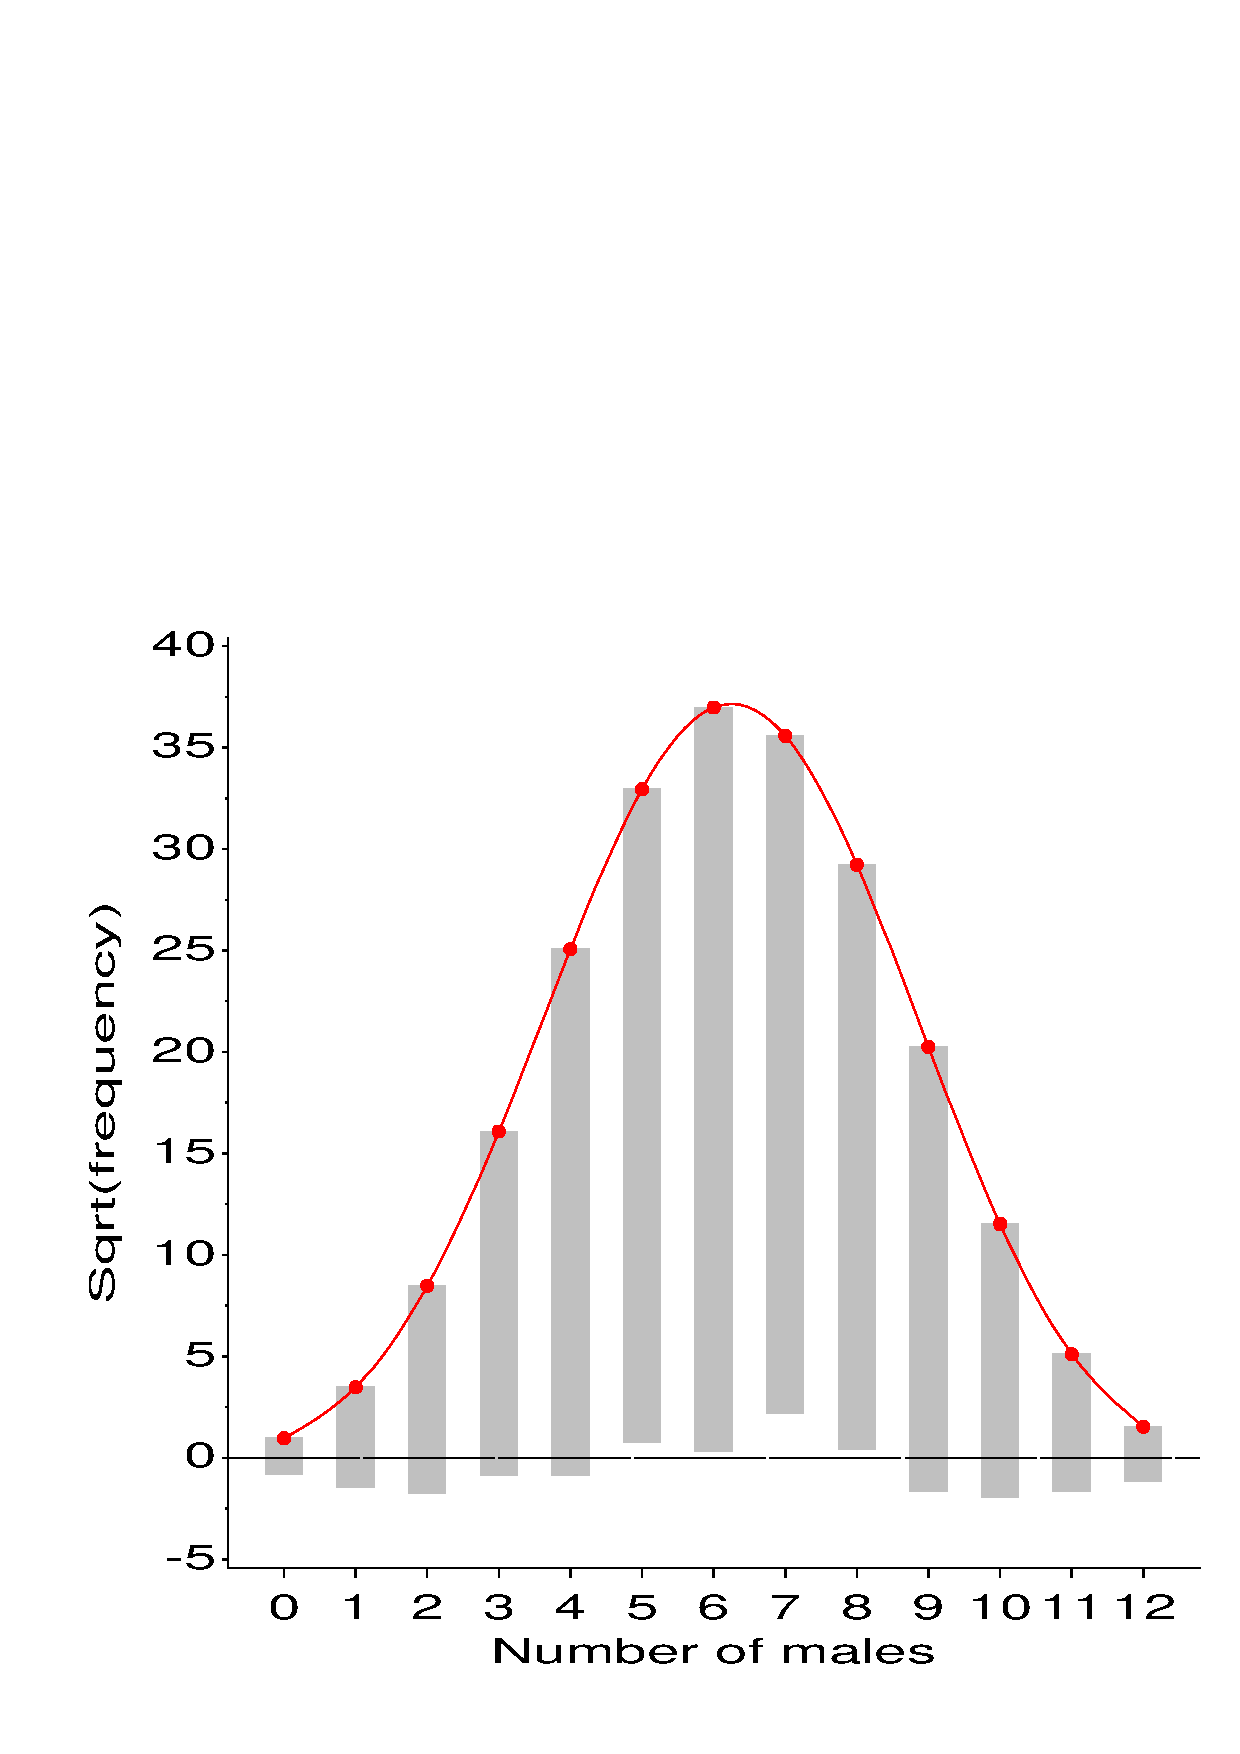
\includegraphics[width=1\linewidth]{saxony}\graphicsfile{ch2/fig/saxony.eps}{}
 \end{minipage}%
 \hfill
 \begin{minipage}[c]{.33\linewidth}
  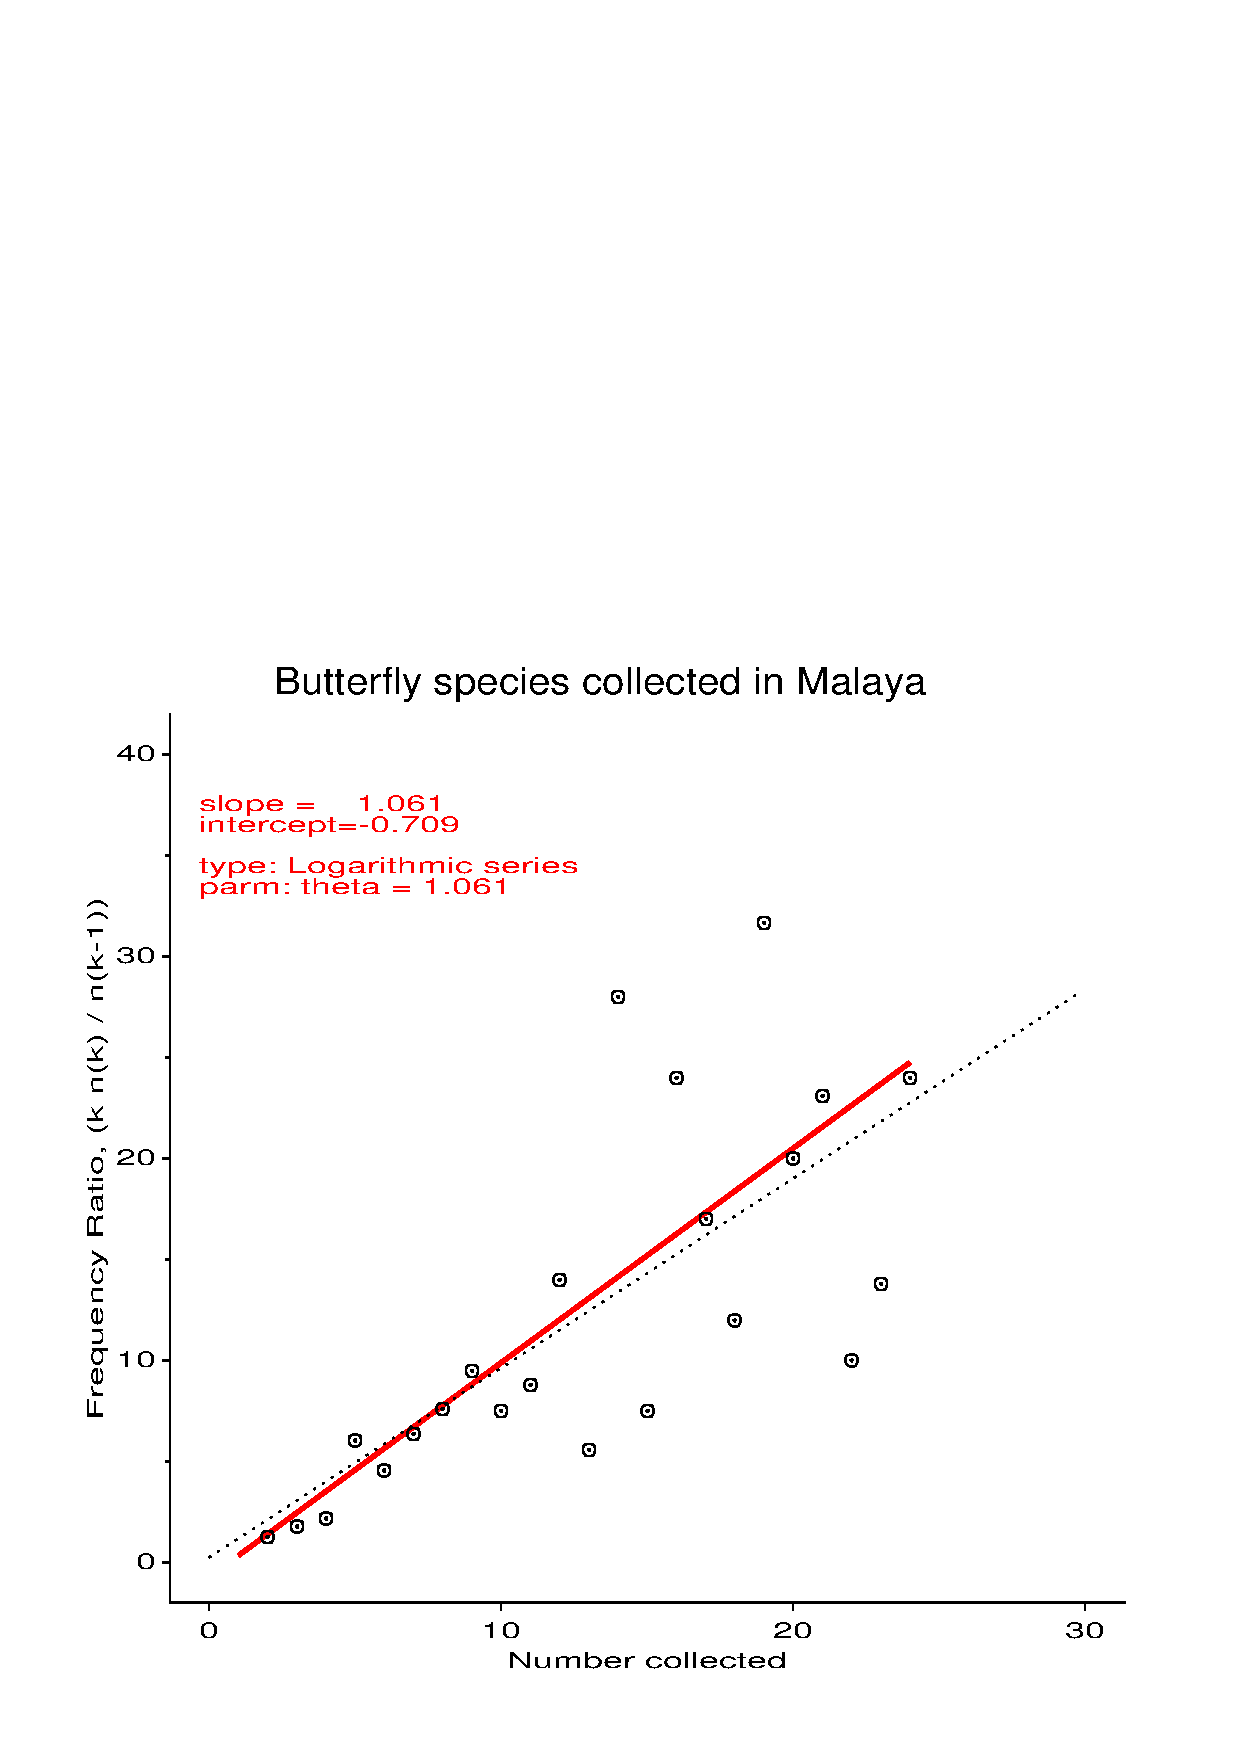
\includegraphics[width=1\linewidth]{orddemo3}\graphicsfile{ch2/fig/orddemo3.eps}{}
 \end{minipage}
 \hfill
 \begin{minipage}[c]{.33\linewidth}
  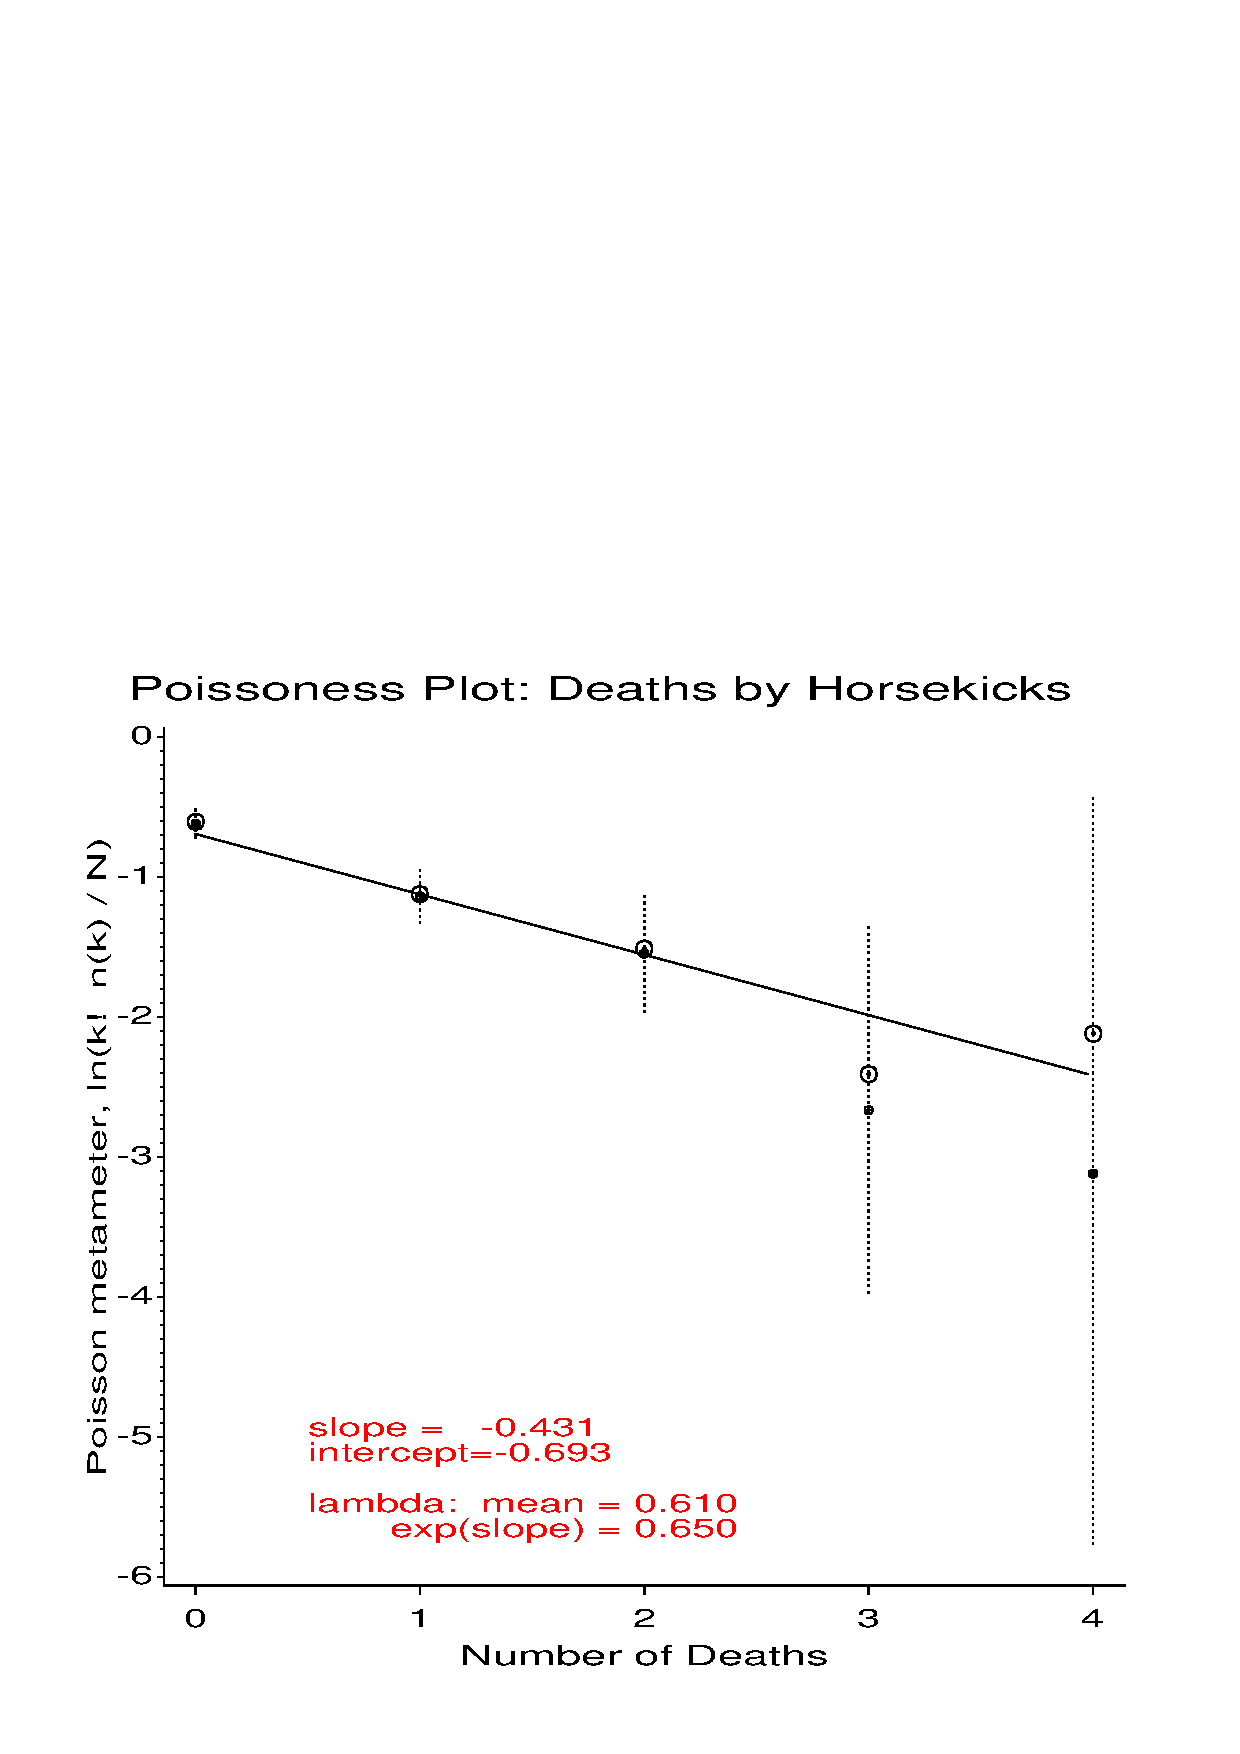
\includegraphics[width=1\linewidth]{poisdemo1}\graphicsfile{ch2/fig/poisdemo1.eps}{}
 \end{minipage}
\end{center}

		% visual table of contents

\chapterprelude{
The analysis of two-way frequency tables concerns the association
between two variables.  A variety of specialized graphical
displays help to visualize the pattern of association,
using area of some region to represent the frequency in a cell.
Some of these methods are focused
on visualizing an odds ratio (for $2 \times 2$ tables), or the general
pattern of association, or the agreement between row and column
categories in square tables.}
% \minitoc
% \clearpage

\section{Introduction}\label{sec:twoway-intro}
\epigraph{Tables are like cobwebs, like the
sieve of Danaides; beautifully reticulated, orderly to look upon, but
which will hold no conclusion. Tables are abstractions, and the object a most
concrete one, so difficult to read the essence of.}{From \emph{Chartism} by Thomas Carlyle \citeyearpar{Carlyle:1840}, Chapter II, Statistics}

Most methods of statistical analysis are concerned with understanding
relationships or dependence among variables.
With categorical variables, these relationships are often
studied from data which has been
summarized by a \term{contingency table}
in table form or frequency form,
giving the frequencies of observations cross-classified
by two or more such variables. As Thomas Carlyle said, it is often difficult
to appreciate the message conveyed in numerical tables.

This chapter is concerned with simple graphical methods for understanding the association
between two categorical variables.
Some examples are also presented which involve a third, \term{stratifying variable},
where we wish to determine if the relationship between two primary
variables is the same or different for all levels of the
stratifying variable.
More general methods for fitting models and displaying associations for three-way
and larger tables are described in \chref{ch:mosaic}.

In \secref{sec:twoway-tests}, We describe briefly some numerical
and statistical
methods for testing whether an association
exists between two variables,  and measures
for quantifying the strength
of this association.
In \secref{sec:twoway-strat} we extend these ideas to situations where
the relation between two variables is of primary interest, but there
are one or more background variables to be controlled.

The main emphasis, however, is on graphical methods which help
to describe the \emph{pattern} of an association between variables.
\secref{sec:twoway-fourfold} presents the fourfold display,
designed to portray the odds ratio in $2 \times 2$ tables or a set
of $k$ such tables.
\boldital{Sieve diagrams}\ix{sieve diagrams}
(\secref{sec:twoway-sieve}) and \term{association plots}
(\secref{sec:twoway-assoc}) are more general methods for depicting
the pattern of associations an any two-way tables.
When the row and column variables represent the classifications
of different raters, specialized measures and visual displays
for \term{inter-rater agreement} (\secref{sec:twoway-agree}) are particularly
useful.
Another specialized display, a \term{trilinear plot} or \term{ternary plot},
described in \secref{sec:twoway-trilinear},
is designed
for three-column frequency tables or compositional data.
In order to make clear some of the distinctions which occur in
\ctab analysis, we begin with several examples.

\begin{Example}[berkeley1]{Berkeley admissions}
\tabref{tab:berk22} shows aggregate data on applicants to
graduate school at Berkeley for the six largest departments in 1973
classified by admission and gender
\citep{Bickel-etal:75}.
See \data{UCBAdmissions} (in package \pkg{datasets}) for the complete data set.
For such data we might wish to study whether there is an association
between admission and gender.
Are male (or female) applicants more likely to be admitted?
The presence of an association might be considered as
evidence of sex bias in admission practices.

\tabref{tab:berk22} is an example of the simplest kind of \ctab,
a $2 \times 2$ classification of individuals according to two
dichotomous (binary) variables.
For such a table, the question of whether there is an association
between admission and gender is equivalent to asking if the
proportions of males and females who are admitted to graduate
school are the different, or whether the difference in proportions
admitted is not zero.
\begin{table}[htb]
\caption{Admissions to Berkeley graduate programs}
\label{tab:berk22}
 \begin{center}
\begin{tabular}{lrr|rrr}
\hline
  & Admitted & Rejected & Total & \red{\% Admit} & \red{Odds(Admit)}\\
\hline
 Males & 1198 & 1493 & 2691  & \red{44.52} & \red{0.802}\\
 Females & 557 & 1278 & 1835 & \red{30.35} & \red{0.437}\\
\hline
 Total & 1755 & 2771 & 4526  & 38.78 & 0.633\\
\hline
\end{tabular}
\end{center}
\end{table}

\end{Example}

Although the methods for quantifying association in larger tables can be
used for $2 \times 2$ tables, there are specialized measures
(described in \secref{sec:twoway-tests}) and
graphical methods for these simpler tables.

As we mentioned in \secref{sec:exp-resp}
it is often useful to make a distinction between \term{response},
or outcome variables, on the one hand,
and possible \term{explanatory}
or predictor variables on the other.
In \tabref{tab:berk22}, it is natural to consider \var{admission}
as the outcome, and \var{gender} as the explanatory variable.
In other tables, no variable may be clearly identified as \emph{the}
outcome, or there may be several response variables, giving a
multivariate problem.

\begin{Example}[haireye1]{Hair color and eye color}
\tabref{tab:hairdat} shows data collected by
\citet{Snee:74}
on the relation between hair color and eye color among 592
students in a statistics course
(a two-way margin of \data{HairEyeColor}).
\begin{table}[htb]

\caption{Hair-color eye-color data}\label{tab:hairdat}
\begin{center}
\begin{tabular}{|lrrrr|r|}
\hline
        & \multicolumn{4}{c|}{Hair Color}        & \\
Eye     &         &         &         &         &       \\
Color   &  Black  &  Brown  &    Red  &  Blond  & Total \\[2ex] \hline
Green   &      5  &     29  &     14  &     16  &    64 \\
Hazel   &     15  &     54  &     14  &     10  &    93 \\
Blue    &     20  &     84  &     17  &     94  &   215 \\
Brown   &     68  &    119  &     26  &      7  &   220 \\[1ex] \hline
Total   &    108  &    286  &     71  &    127  &   592 \\ \hline
\end{tabular}
\end{center}
\end{table}


Neither hair color nor eye color
is considered a response in relation to the other;  our interest concerns
whether an association exists between them.
Hair color and eye color have both been classified
into four categories.  Although the categories used are among the most
common, they are not the only categories possible.%
\footnote{If students had been asked to write down their hair and eye
colors, it is likely that many more than four categories of each
would appear in a sample of nearly 600.}
A common, albeit deficient, representation of such a table is a
\term{grouped barchart}, as shown in the left of \figref{fig:bartile}: 
\begin{knitrout}
\definecolor{shadecolor}{rgb}{1, 0.961, 0.933}\color{fgcolor}\begin{kframe}
\begin{alltt}
\hlstd{> }\hlstd{hec} \hlkwb{<-} \hlkwd{margin.table}\hlstd{(HairEyeColor,} \hlnum{2}\hlopt{:}\hlnum{1}\hlstd{)}
\hlstd{> }\hlkwd{barplot}\hlstd{(hec,} \hlkwc{beside} \hlstd{=} \hlnum{TRUE}\hlstd{,} \hlkwc{legend} \hlstd{=} \hlnum{TRUE}\hlstd{)}
\end{alltt}
\end{kframe}
\end{knitrout}
\begin{knitrout}
\definecolor{shadecolor}{rgb}{1, 0.961, 0.933}\color{fgcolor}\begin{figure}[!htbp]

\centerline{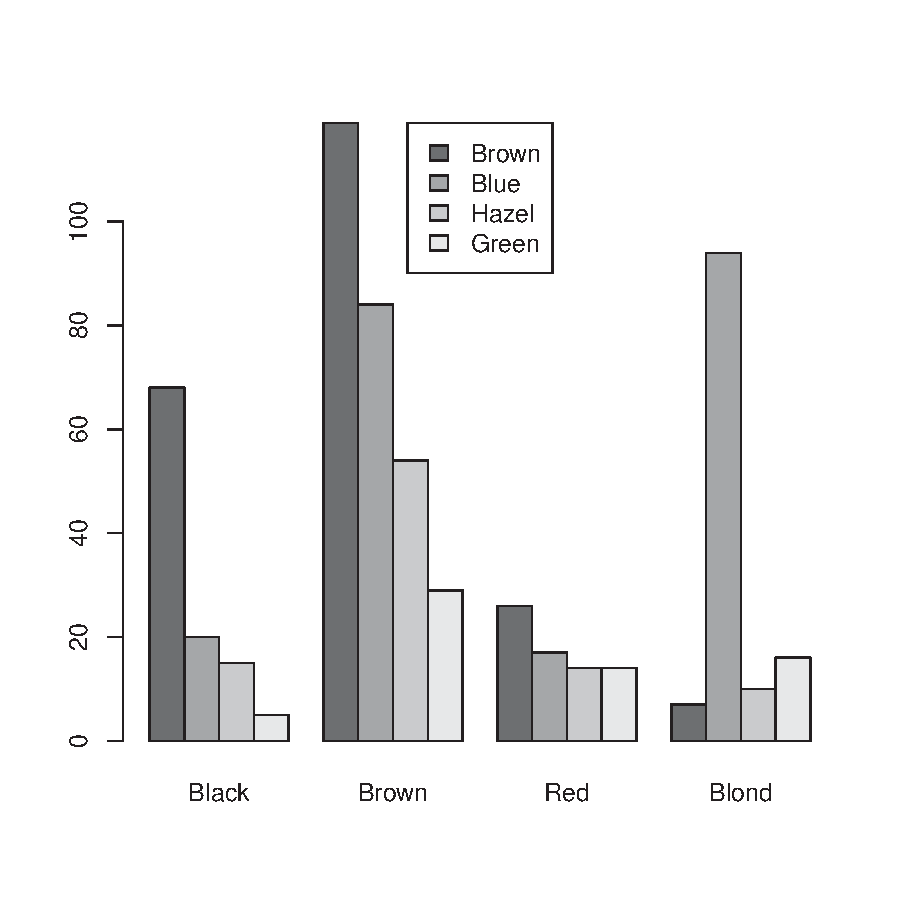
\includegraphics[width=.49\textwidth]{ch04/fig/bartile-1} 
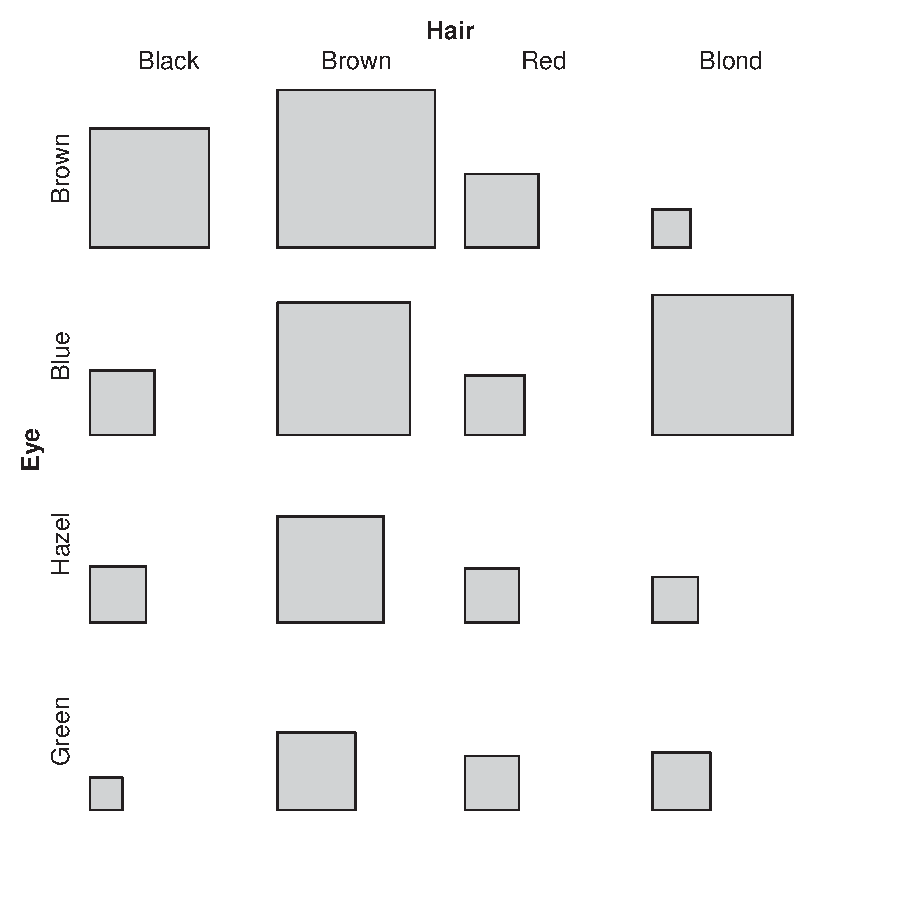
\includegraphics[width=.49\textwidth]{ch04/fig/bartile-2} }

\caption[Two basic displays for the Hair-color Eye-color data]{Two basic displays for the Hair-color Eye-color data. Left: grouped barchart; right: tile plot.\label{fig:bartile}}
\end{figure}


\end{knitrout}
\noindent For each hair
color, a group of bars represent the corresponding eye colors, the
heights being proportional to the absolute frequencies. Bar graphs do
not extend well to more than one dimension since
\begin{itemize}
\item the graphical representation does not match the tabular data structure,
  complicating comparisons with the raw data;
\item it is harder to compare bars accross groups than within groups;
\item by construction, the grouping suggests a conditional
or causal relationship of the variables (here: ``what is the eye color
  \emph{given} the hair color?'', ``how does eye color influence hair color?''), even
  though such an interpretation may be inappropriate (as in this example);
\item labeling may become increasingly complex.
\end{itemize}
A somewhat better approach is a \term{tile plot} (using \func{tile} in \pkg{vcd}), as shown next to the bar
plot in \figref{fig:bartile}:
\begin{knitrout}
\definecolor{shadecolor}{rgb}{1, 0.961, 0.933}\color{fgcolor}\begin{kframe}
\begin{alltt}
\hlstd{> }\hlkwd{tile}\hlstd{(hec)}
\end{alltt}
\end{kframe}
\end{knitrout}
\noindent The table frequencies are represented by the area of
rectangles arranged in the same tabular form than the raw data,
facilitating comparisons between tiles accross both variables (by rows
or by columns), by maintaining a one-to-one relationship to the
underlying table
\footnote{This kind of displays are more generally known as
\term{fluctuation diagrams} \citep{Hofmann:00}, 
flexibly implemented by function \func{fluctile} in package \pkg{extracat}.}.

Everyday observation suggests that there probably is an association
between hair color and eye color, and we will describe tests
and measures of associations for larger tables in
\secref{sec:twoway-overall}.
If, as is suspected, hair color and eye color are associated,
we would like to understand \emph{how} they are associated.
The graphical methods described later in this chapter
and in \chref{ch:mosaic} help
reveal the pattern of associations present.
\end{Example}

\begin{Example}[mental1]{Mental impairment and parents' SES}
\citet[p. 289]{Srole-etal:78} gave the data
in \tabref{tab:mental-tab} on the mental
health status of a sample of 1660 young New York residents in midtown Manhattan
classified by their parents' socioeconomic status (SES);
see \data{Mental} in the \Rpackage{vcdExtra}.
These data have also been analyzed by many authors, including
\citet[ \S 10.5.3]{Agresti:2013},
\citet{Goodman:79}, and
\citet[p. 375]{Haberman:79}.

There are six categories of SES (from 1 $=$ ``High'' to 6 $=$ ``Low''), and mental health is classified
in the four categories ``well'', ``mild symptom formation'',
``moderate symptom formation'', and ``impaired''.
It may be useful here to consider SES as explanatory
and ask whether and how it predicts mental health status as
a response, that is, whether there is an association, and if so, investigate
its nature.

% latex table generated in R 3.0.1 by xtable 1.7-1 package
% Fri Dec 20 17:19:39 2013
\begin{table}[!b]
\centering
\caption{Mental impairment and parents' SES} \label{tab:mental-tab}
\begin{tabular}{r|rrrr}
  \hline
    & \multicolumn{4}{c}{Mental impairment} \\
SES & Well & Mild & Moderate & Impaired \\ 
  \hline
  1 & 64 & 94 & 58 & 46 \\ 
  2 & 57 & 94 & 54 & 40 \\ 
  3 & 57 & 105 & 65 & 60 \\ 
  4 & 72 & 141 & 77 & 94 \\ 
  5 & 36 & 97 & 54 & 78 \\ 
  6 & 21 & 71 & 54 & 71 \\ 
   \hline
\end{tabular}
\end{table}

\begin{knitrout}
\definecolor{shadecolor}{rgb}{1, 0.961, 0.933}\color{fgcolor}\begin{kframe}
\begin{alltt}
\hlstd{> }\hlkwd{data}\hlstd{(Mental,} \hlkwc{package} \hlstd{=} \hlstr{"vcdExtra"}\hlstd{)}
\hlstd{> }\hlstd{mental} \hlkwb{<-} \hlkwd{xtabs}\hlstd{(Freq} \hlopt{~} \hlstd{ses} \hlopt{+} \hlstd{mental,} \hlkwc{data} \hlstd{= Mental)}
\hlstd{> }\hlkwd{spineplot}\hlstd{(mental)}
\end{alltt}
\end{kframe}\begin{figure}[!htbp]

\centerline{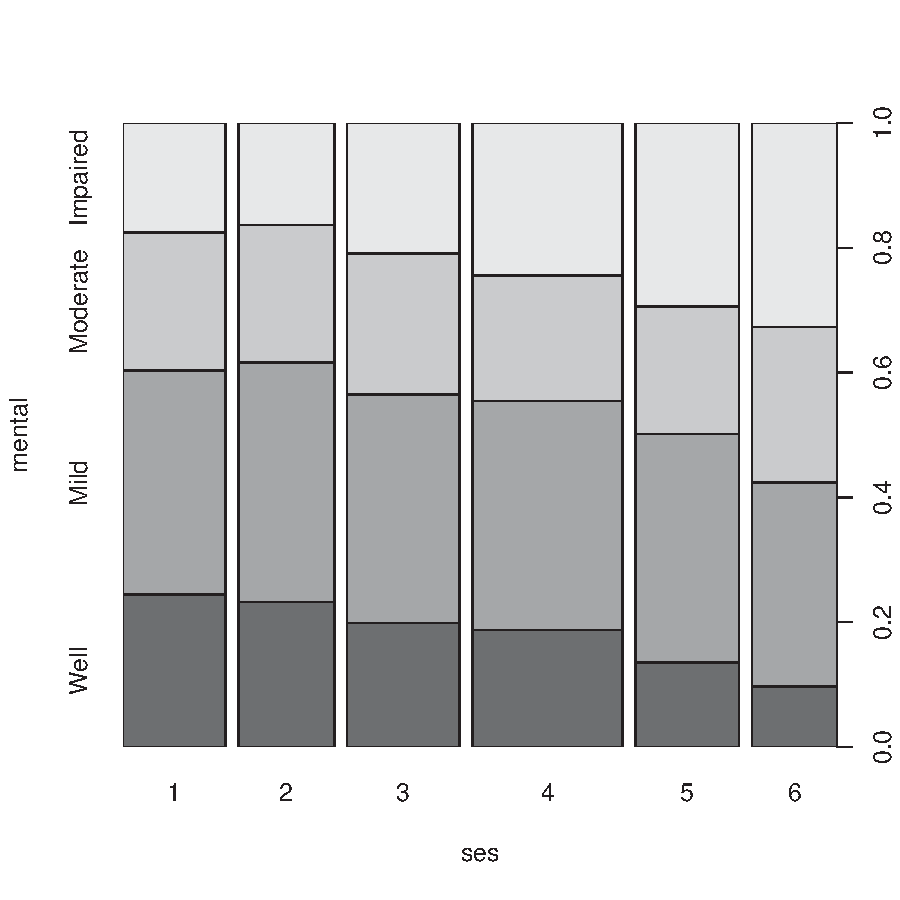
\includegraphics[width=0.7\textwidth]{ch04/fig/spineplot-1} }

\caption[Spineplot of the Mental data]{Spineplot of the Mental data.\label{fig:spineplot}}
\end{figure}


\end{knitrout}
\figref{fig:spineplot} shows a \term{spineplot} of this
data---basically a stacked barchart of the row percentages of mental
impairment for each SES category, the width of each bar being proportional to
the overall SES percentages.\footnote{Thus, in the more technical terms introduced in \ref{sec:twoway-notation}, 
this spineplot shows the conditional distribution of impairment, given
the categories of SES.}
From this graph, it is apparant that the ``well'' mental state decreases with
social-economic status, while the ``impaired'' state increases. This
pattern is more specific than overall association (as
suspected for the hair-color eye-color data), and indeed, more powerful and focused tests are available
when we treat these variables as \emph{ordinal}, as we will see in
\secref{sec:ordinaltests}.
\end{Example}

\begin{Example}[arthrit1]{Arthritis treatment}
The data in \tabref{tab:arthrit} compares an active treatment for rheumatoid
arthritis to a placebo
\citep{KochEdwards:88}, used in examples in \chref{ch:working}
(\exref{ex:ch2-arth}).
The outcome reflects
whether individuals showed no improvement, some improvement, or
marked improvement.
Here, the outcome variable is an ordinal one, and it is probably
important to determine if the relation between treatment and outcome
is the same for males and females.
The data set is given in case form in \data{Arthritis} (in package \pkg{vcd}).
\begin{table}[tb]

\caption{Arthritis treatment data}\label{tab:arthrit}
\begin{center}
\begin{tabular}{ll|rrr|r}
\hline
     &  & \multicolumn{3}{c|}{Improvement}            &  \\
\hline
   Treatment&  Sex    &None    &Some    &Marked  &  Total \\[2ex]
\hline
   Active   &  Female &      6 &      5 &     16 &     27 \\
            &  Male   &      7 &      2 &      5 &     14 \\
\hline
   Placebo  &  Female &     19 &      7 &      6 &     32 \\
            &  Male   &     10 &      0 &      1 &     11 \\[1ex]
\hline
   Total    &         &     42 &     14 &     28 &     84 \\
\hline
\end{tabular}
\end{center}
\end{table}



This is, of course, a three-way table, with factors
\var{Treatment}, \var{Sex}, and \var{Improvement}.
If the relation between treatment and outcome is the same for
both genders, an analysis of the Treatment by Improvement
table (collapsed over sex) could be carried out.
Otherwise we could perform separate analyses for
men and women, or
treat the combinations of treatment and sex as four levels of
a ``population'' variable, giving a $4 \times 3$ two-way table.
These simplified approaches each ignore certain information
available in
an analysis of the full three-way table.
\end{Example}

\section{Tests of association for two-way tables}\label{sec:twoway-tests}

\subsection{Notation and terminology}\label{sec:twoway-notation}
To establish notation, let \(\mat{N}  =  \{  n_{ij}  \}\) be the
observed frequency table of variables \(A\) and \(B\) with \(r\) rows
and \(c\) columns, as shown in \tabref{tab:rbyc}.
In what follows, a subscript is replaced by a ``$+$''
when summed over the corresponding variable, so \(n_{i+}  =  \sum_j \,
n_{ij}\) gives the total frequency in row \(i\), \(n_{+j}  =  \sum_i \,
n_{ij}\) gives the total frequency in column \(j\), and \(n_{++}  =
\sum_i \sum_j \,  n_{ij}\) is the grand total; for convenience,
\(n_{++}\) is also symbolized by \(n\).
\begin{table}[htb]
\caption[The R by C contingency table]{The $R \times C$ contingency table}
\label{tab:rbyc}
\vspace{1ex}
\begin{center}
\begin{tabular}{l|llll|l}
\hline
Row      & \multicolumn{4}{c|}{Column category}      &          \\
Category &   1      &   2      & $\cdots$  &  $C$    & Total    \\
\hline
   1     & $n_{11}$ & $n_{12}$ & $\cdots$ & $n_{1C}$ & $n_{1+}$ \\
   2     & $n_{21}$ & $n_{22}$ & $\cdots$ & $n_{2C}$ & $n_{2+}$ \\
$\vdots$ & $\vdots$ & $\vdots$ & $\cdots$ & $\vdots$ & $\vdots$ \\
   $R$   & $n_{R1}$ & $n_{R2}$ & $\cdots$ & $n_{RC}$ & $n_{R+}$   \\  
\hline
Total    & $n_{+1}$ & $n_{+2}$ & $\cdots$ & $n_{+C}$ & $n_{++}$   \\
\hline
\end{tabular}
\end{center}
\end{table}

When each observation is randomly sampled from some population
and classified on two categorical variables, $A$ and $B$,
we refer to the \term{joint distribution} of these variables,
and let $\pi_{ij} = \Pr(A=i,\,B=j)$ denote the population
probability that
an observation is classified in row $i$, column $j$ (or cell $(ij)$)
in the table.
Corresponding to these population joint probabilities, the
cell proportions, $p_{ij} = n_{ij} / n$, give the sample joint
distribution.

The row totals $n_{i+}$ and column totals $n_{+j}$ are called
\term{marginal frequencies} for variables $A$ and $B$ respectively.
These describe the distribution of each variable \emph{ignoring} the other.
For the population probabilities, the \term{marginal distributions}
are defined analogously as the row and column totals of the
joint probabilities,
$\pi_{i+} = \sum_j \pi_{ij}$, and
$\pi_{+j} = \sum_i \pi_{ij}$.
The sample marginal proportions are, correspondingly,
$p_{i+} = \sum_j p_{ij} = n_{i+} / n$, and
$p_{+j} = \sum_i p_{ij} = n_{+j} / n$.

When one variable (the column variable, $B$, for example) is a response
variable, and the other ($A$) is an explanatory variable,
it is most often useful to examine the distribution of the response $B$
for \emph{each} level of $A$ separately.
These define the \term{conditional distributions} of $B$, given the
level of $A$, and are defined for the population as
$\pi_{j\given i} = \pi_{ij} / \pi_{i+}$.

These definitions are illustrated
for the Berkeley data (\tabref{tab:berk22}) below,
using the function \func{CrossTable}.
\begin{knitrout}
\definecolor{shadecolor}{rgb}{1, 0.961, 0.933}\color{fgcolor}\begin{kframe}
\begin{alltt}
\hlstd{> }\hlstd{Berkeley} \hlkwb{<-} \hlkwd{margin.table}\hlstd{(UCBAdmissions,} \hlnum{2}\hlopt{:}\hlnum{1}\hlstd{)}
\hlstd{> }\hlkwd{library}\hlstd{(gmodels)}
\hlstd{> }\hlkwd{CrossTable}\hlstd{(Berkeley,} \hlkwc{prop.chisq} \hlstd{=} \hlnum{FALSE}\hlstd{,} \hlkwc{prop.c} \hlstd{=} \hlnum{FALSE}\hlstd{,} \hlkwc{format} \hlstd{=} \hlstr{"SPSS"}\hlstd{)}
\end{alltt}
\begin{verbatim}

   Cell Contents
|-------------------------|
|                   Count |
|             Row Percent |
|           Total Percent |
|-------------------------|

Total Observations in Table:  4526 

             | Admit 
      Gender | Admitted  | Rejected  | Row Total | 
-------------|-----------|-----------|-----------|
        Male |     1198  |     1493  |     2691  | 
             |   44.519% |   55.481% |   59.456% | 
             |   26.469% |   32.987% |           | 
-------------|-----------|-----------|-----------|
      Female |      557  |     1278  |     1835  | 
             |   30.354% |   69.646% |   40.544% | 
             |   12.307% |   28.237% |           | 
-------------|-----------|-----------|-----------|
Column Total |     1755  |     2771  |     4526  | 
-------------|-----------|-----------|-----------|

 
\end{verbatim}
\end{kframe}
\end{knitrout}
The output shows the joint frequencies, $n_{ij}$, and joint sample percentages,
$100 \times p_{ij}$, in the first row within each table cell.
The second row in each cell (``Row percent'')
gives the conditional percentage of admission or rejection,
$100 \times p_{j\given i}$ for males and females separately.
The row and column labelled ``Total'' give the
marginal frequencies, $n_{i+}$ and $n_{+j}$,
and marginal percentages, $p_{i+}$ and $p_{+j}$.


%\section{Stratified analysis}\label{sec:twoway-strat}

\subsection{2 by 2 tables: Odds and odds ratios}\label{sec:twoway-twobytwo}

The $2 \times 2$ \ctab of applicants to Berkeley graduate programs in \tabref{tab:berk22} may be regarded as an example of a
\term{cross-sectional study}.
The total of $n = 4,526$ applicants in 1973 has been classified by both
gender and admission status.
Here, we would probably consider the total $n$ to be fixed,
and the cell frequencies $n_{ij},  \: i=1,2; j=1,2$
would then represent a single
\term{multinomial sample} for the cross-classification by two
binary variables,
with probabilities cell $p_{ij},  \: i=1,2; j=1,2$
such that
\begin{equation*}
 p_{11} + p_{12} + p_{21} + p_{22} = 1
 \period
\end{equation*}
The basic null hypothesis of interest for a multinomial sample is that
of \emph{independence}.  Are admission and gender independent of each other?

Alternatively, if we consider admission the response variable, and
gender an explanatory variable, we would treat the numbers of male
and female applicants as fixed
and consider the cell frequencies to represent two independent
\term{binomial samples} for a binary response.
In this case, the null hypothesis is described as that of \emph{homogeneity}
of the response proportions across the levels of the explanatory variable.

\ixon{odds ratio}
Measures of association are used to quantify the strength of association
between variables.  Among the many measures of association for
\ctabs, the \term{odds ratio} is particularly useful for
$2 \times 2$ tables, and is a fundamental parameter in several
graphical displays and models described later.
Other measures of strength of association for $2 \times 2$ tables
are described in \citet[\C 2]{Stokes-etal:00} and \citet[\S 2.2]{Agresti:96}.

For a binary response, where the probability of a ``success'' is $\pi$,
the \term{odds} of a success is defined as
\begin{equation*}
 \textrm{odds} = \frac{\pi}{1-\pi} \period
\end{equation*}
Hence, $\textrm{odds} = 1$ corresponds to $\pi = 0.5$, or success and
failure equally likely.   When success is more likely than failure
$\pi > 0.5$, and the $\textrm{odds} > 1$;  for instance, when $\pi = 0.75$,
$\textrm{odds} = .75/.25 =3$, so a success is three times as likely
as a failure.  When failure is more likely, $\pi < 0.5$, and the $\textrm{odds} < 1$;  for instance, when $\pi = 0.25$,
$\textrm{odds} = .25/.75 =\frac{1}{3}$.

The odds of success thus vary \emph{multiplicatively} around 1.  Taking logarithms
gives an equivalent measure which varies \emph{additively} around 0, called the
\term{log odds} or \term{logit}:
\begin{equation}\label{eq:logit}
 \logit (\pi) \equiv \log (\mbox{odds}) = \log \left( \frac{\pi}{1-\pi} \right)
 \period
\end{equation}
The logit is symmetric about $\pi = 0.5$, in that
$\logit (\pi) = - \logit (1-\pi)$.  The following lines calculate the odds
and log odds for a range of probabilities. As you will see in
\chref{ch:logistic}, the logit transformation of a probability is fundamental
in logistic regression.

\begin{knitrout}
\definecolor{shadecolor}{rgb}{1, 0.961, 0.933}\color{fgcolor}\begin{kframe}
\begin{alltt}
\hlstd{> }\hlstd{p} \hlkwb{<-} \hlkwd{c}\hlstd{(}\hlnum{0.05}\hlstd{,} \hlnum{.1}\hlstd{,} \hlnum{.25}\hlstd{,} \hlnum{.50}\hlstd{,} \hlnum{.75}\hlstd{,} \hlnum{.9}\hlstd{,} \hlnum{.95}\hlstd{)}
\hlstd{> }\hlstd{odds} \hlkwb{<-} \hlstd{p} \hlopt{/} \hlstd{(}\hlnum{1} \hlopt{-} \hlstd{p)}
\hlstd{> }\hlstd{logodds} \hlkwb{<-} \hlkwd{log}\hlstd{(odds)}
\hlstd{> }\hlkwd{data.frame}\hlstd{(p, odds, logodds)}
\end{alltt}
\begin{verbatim}
     p      odds logodds
1 0.05  0.052632 -2.9444
2 0.10  0.111111 -2.1972
3 0.25  0.333333 -1.0986
4 0.50  1.000000  0.0000
5 0.75  3.000000  1.0986
6 0.90  9.000000  2.1972
7 0.95 19.000000  2.9444
\end{verbatim}
\end{kframe}
\end{knitrout}

A binary response for two groups gives a $2 \times 2$ table, with
Group as the row variable, say.  Let $\pi_1$ and $\pi_2$ be the
success probabilities for Group 1 and Group 2.  The \term{odds ratio}, $\theta$,
is just the ratio of the odds for the two groups:
\begin{equation*}%\label{eq:oddsratio}
 \mbox{odds ratio} \equiv \theta =
 \frac{\mbox{odds}_1} {\mbox{odds}_2} =
 \frac{\pi_1 / (1-\pi_1)} {\pi_2 / (1-\pi_2)}
 \period
\end{equation*}

Like the odds itself, the odds ratio is always non-negative, between
0 and $\infty$.  When $\theta = 1$, the distributions of success and
failure are the same for both groups (so $\pi_1 = \pi_2$);  there is
no association between row and column variables, or the response
is independent of group.
When $\theta > 1$, Group 1 has a greater success probability;
when $\theta < 1$, Group 2 has a greater success probability.

Similarly, the odds ratio may be transformed to a log scale, to give
a measure which is symmetric about 0.
The \term{log odds ratio}, symbolized by $\psi$, is just the difference
between the logits for Groups 1 and 2:
\begin{equation*}%\label{eq:logoddsratio}
 \mbox{log odds ratio} \equiv \psi
 = \log (\theta)
 = \log \left[ \frac{\pi_1 / (1-\pi_1)} {\pi_2 / (1-\pi_2)} \right]
 = \logit (\pi_1) - \logit(\pi_2)
 \period
\end{equation*}
Independence corresponds to $\psi =0$, and reversing the rows or columns
of the table merely changes the sign of $\psi$.

For sample data, the \term{sample odds ratio} is the ratio of the sample
odds for the two groups:
\begin{equation}\label{eq:soddsratio}
 \hat{\theta} =  \frac{p_1 / (1-p_1)} {p_2 / (1-p_2)} =
 \frac{ n_{11} / n_{12} }{ n_{21} / n_{22}} =
 \frac{ n_{11} n_{22} } {n_{12} n_{21}}
 \period
\end{equation}

\begin{comment}
We described the odds ratio for a sampling context of independent binomial
samples, but actually, the odds ratio is an appropriate measure of strength
of association for all the standard sampling schemes, because it treats
the variables symmetrically.  It does not matter whether the row or column
variable is the response, or whether both variables are treated as
responses.  Other measures of strength of association, not described here,
\emph{do} distinguish between explanatory and response variables.
\end{comment}

The sample estimate $\hat{\theta}$ in \eqref{eq:soddsratio} is the
maximum likelihood estimator of the true $\theta$.
The sampling distribution of $\hat{\theta}$ is asymptotically normal
as $n \rightarrow \infty$, but may be highly skewed in small to
moderate samples.

Consequently, inference for the odds ratio
is more conveniently carried out in terms of the log odds ratio,
whose sampling distribution is more closely normal, with mean
$\psi = \log (\theta)$, and asymptotic standard error (ASE)
\begin{equation}\label{eq:aselogtheta}
 \mbox{ASE }_{\log (\theta)} \equiv \hat{s} (\hat{\psi}) = \sqrt{
 \frac{1}{n_{11}} + \frac{1}{n_{12}} + \frac{1}{n_{21}} + \frac{1}{n_{22}}
 }
 =   \sqrt{ \sum_{i,j} n_{ij}^{-1}}
\end{equation}
A large-sample $100(1-\alpha)$\% confidence interval for $\log (\theta)$ may therefore
be calculated as
\begin{equation*}
\log (\theta) \pm z_{1-\alpha/2} \, \mbox{ASE }_{\log (\theta)}
= \hat{\psi} \pm z_{1-\alpha/2}  \, \hat{s} (\hat{\psi})
\end{equation*}
where $z_{ 1 - \alpha  / 2 }$ is the cumulative normal quantile with
$1-\alpha/2$ in the lower tail.
Confidence intervals for $\theta$ itself are obtained by exponentiating
the end points of the interval for $\psi = \log (\theta)$,%
\footnote{
Note that $\hat{\theta}$ is 0 or $\infty$ if any $n_{ij}=0$.
\citet{Haldane:55} and \citet{GartZweiful:67} showed that improved
estimators of $\theta$ and $\psi = \log (\theta)$ are obtained by
replacing each $n_{ij}$ by $[n_{ij} + \frac{1}{2}]$ in \eqref{eq:soddsratio}
and \eqref{eq:aselogtheta}.
This adjustment is preferred in small samples, and required if any
zero cells occur.  In large samples, the effect of adding 0.5 to each
cell becomes negligible.
}
\begin{equation*}
\exp \left(\hat{\psi}  \pm z_{ 1 - \alpha  / 2 } \hat{s} (\hat{\psi}) \right)
\period
\end{equation*}

\begin{Example}[ucbadmissions]{UCB Admissions}
As an illustratation, we apply these formulae to the UCB Admissions
data, using the \func{oddsratio} function in \pkg{vcd} (Note that by
default log-odds are calculated): \TODO{Better use loddsratio here}
\begin{knitrout}
\definecolor{shadecolor}{rgb}{1, 0.961, 0.933}\color{fgcolor}\begin{kframe}
\begin{alltt}
\hlstd{> }\hlkwd{data}\hlstd{(UCBAdmissions)}
\hlstd{> }\hlstd{UCB} \hlkwb{<-} \hlkwd{margin.table}\hlstd{(UCBAdmissions,} \hlnum{1}\hlopt{:}\hlnum{2}\hlstd{)}
\hlstd{> }\hlstd{(OR} \hlkwb{<-} \hlkwd{oddsratio}\hlstd{(UCB,} \hlkwc{log} \hlstd{=} \hlnum{FALSE}\hlstd{))}
\end{alltt}
\begin{verbatim}
[1] 1.8411
\end{verbatim}
\begin{alltt}
\hlstd{> }\hlstd{(LOR} \hlkwb{<-} \hlkwd{oddsratio}\hlstd{(UCB))}
\end{alltt}
\begin{verbatim}
[1] 0.61035
\end{verbatim}
\end{kframe}
\end{knitrout}
\noindent The function returns an object for which the \func{summary}
method computes the ASE and carries out the significance test (for the
log odds):
\begin{knitrout}
\definecolor{shadecolor}{rgb}{1, 0.961, 0.933}\color{fgcolor}\begin{kframe}
\begin{alltt}
\hlstd{> }\hlkwd{summary}\hlstd{(LOR)}
\end{alltt}
\begin{verbatim}
     Log Odds Ratio Std. Error z value Pr(>|z|)    
[1,]         0.6104     0.0639    9.55   <2e-16 ***
---
Signif. codes:  0 '***' 0.001 '**' 0.01 '*' 0.05 '.' 0.1 ' ' 1
\end{verbatim}
\end{kframe}
\end{knitrout}
\noindent Clearly, the hypothesis of independence has to be rejected,
suggesting the presence of gender bias.
\func{confint} computes confidence intervals for (log) odds ratios:
\begin{knitrout}
\definecolor{shadecolor}{rgb}{1, 0.961, 0.933}\color{fgcolor}\begin{kframe}
\begin{alltt}
\hlstd{> }\hlkwd{confint}\hlstd{(OR)}
\end{alltt}
\begin{verbatim}
        lwr    upr
[1,] 1.6244 2.0867
\end{verbatim}
\begin{alltt}
\hlstd{> }\hlkwd{confint}\hlstd{(LOR)}
\end{alltt}
\begin{verbatim}
         lwr     upr
[1,] 0.48512 0.73558
\end{verbatim}
\end{kframe}
\end{knitrout}
\noindent Finally, we note that an exact test (based on the
hypergeometric distribution) is provided by
\func{fisher.test} (see the help page for the details):
\begin{knitrout}
\definecolor{shadecolor}{rgb}{1, 0.961, 0.933}\color{fgcolor}\begin{kframe}
\begin{alltt}
\hlstd{> }\hlkwd{fisher.test}\hlstd{(UCB)}
\end{alltt}
\begin{verbatim}

	Fisher's Exact Test for Count Data

data:  UCB
p-value < 2.2e-16
alternative hypothesis: true odds ratio is not equal to 1
95 percent confidence interval:
 1.6214 2.0912
sample estimates:
odds ratio 
    1.8409 
\end{verbatim}
\end{kframe}
\end{knitrout}
\noindent In general, exact tests are to be prefered over asymptotic tests
like the one described above. Note, however, that the results are very
similar in this example.
\end{Example} 
\ix{Fisher's exact test}
\ixoff{odds ratio}

\subsection{Larger tables: Overall analysis}\label{sec:twoway-overall}

For two-way tables overall tests of association can be carried out
using \func{assocstats}.
If the data set has more than two factors (as in the
\data{Arthritis} data), the other factors will be
ignored (and collapsed) if not included when the table is constructed.
This simplified analysis may be misleading if
the excluded factors interact with the factors used in the
analysis.

\begin{Example}[arthrit2]{Arthritis treatment}
Since the main interest is in the relation between \var{Treatment} and
\var{Improved}, an overall analysis (which ignores \var{Sex}) can be carried out
by creating a two-way table with \func{xtabs}
as shown below.
\ixd{arthritis treatment}
\begin{knitrout}
\definecolor{shadecolor}{rgb}{1, 0.961, 0.933}\color{fgcolor}\begin{kframe}
\begin{alltt}
\hlstd{> }\hlkwd{data}\hlstd{(}\hlstr{"Arthritis"}\hlstd{,} \hlkwc{package}\hlstd{=}\hlstr{"vcd"}\hlstd{)}
\hlstd{> }\hlstd{Art} \hlkwb{<-} \hlkwd{xtabs}\hlstd{(}\hlopt{~} \hlstd{Treatment} \hlopt{+} \hlstd{Improved,} \hlkwc{data} \hlstd{= Arthritis)}
\hlstd{> }\hlstd{Art}
\end{alltt}
\begin{verbatim}
         Improved
Treatment None Some Marked
  Placebo   29    7      7
  Treated   13    7     21
\end{verbatim}
\begin{alltt}
\hlstd{> }\hlkwd{round}\hlstd{(}\hlnum{100} \hlopt{*} \hlkwd{prop.table}\hlstd{(Art,} \hlkwc{margin} \hlstd{=} \hlnum{1}\hlstd{),} \hlnum{2}\hlstd{)}
\end{alltt}
\begin{verbatim}
         Improved
Treatment  None  Some Marked
  Placebo 67.44 16.28  16.28
  Treated 31.71 17.07  51.22
\end{verbatim}
\end{kframe}
\end{knitrout}
The row proportions show a clear difference in the outcome for the two groups:
For those given the placebo, 67\% reported no improvement;
in the treated group, 51\% reported marked improvement.  $\chi^2$ tests
and measures of association are provided by \func{assocstats} as shown below:
\begin{knitrout}
\definecolor{shadecolor}{rgb}{1, 0.961, 0.933}\color{fgcolor}\begin{kframe}
\begin{alltt}
\hlstd{> }\hlkwd{assocstats}\hlstd{(Art)}
\end{alltt}
\begin{verbatim}
                    X^2 df  P(> X^2)
Likelihood Ratio 13.530  2 0.0011536
Pearson          13.055  2 0.0014626

Phi-Coefficient   : 0.394 
Contingency Coeff.: 0.367 
Cramer's V        : 0.394 
\end{verbatim}
\end{kframe}
\end{knitrout}
\end{Example}
\noindent The measures of association are normalized variants of the
$\chi^2$ statistic. The $\phi$ coefficient, for example, is just
$\chi^2/n$. Caution is needed for interpretation since the maximum
values depend on the table dimensions.

\subsection{Tests for ordinal variables}\label{sec:ordinaltests}

For \(r \times  c\) tables, more sensitive tests
than the test for general association (independence)
are available if
either or both of the row and column variables are
ordinal. Generalized \term{Cochran-Mantel-Haenszel tests}
\citep{Landis-etal:1978}
which take the ordinal nature of a variable into
account are provided by the \func{CMHtest} in \pkg{vcdExtra}.
These tests are based on assigning numerical scores to
the table categories;  the default (table) scores treat the levels as
equally spaced.  They generally have higher power when the pattern of
association is determined by the order of an ordinal variable.

\begin{Example}[mental2]{Mental impairment and parents' SES}
We illustrate these tests using the data on mental impairment and SES
introduced in \exref{ex:mental1}, where both variables can be considered ordinal.
\begin{knitrout}
\definecolor{shadecolor}{rgb}{1, 0.961, 0.933}\color{fgcolor}\begin{kframe}
\begin{alltt}
\hlstd{> }\hlkwd{data}\hlstd{(Mental,} \hlkwc{package}\hlstd{=}\hlstr{"vcdExtra"}\hlstd{)}
\hlstd{> }\hlstd{mental} \hlkwb{<-} \hlkwd{xtabs}\hlstd{(Freq} \hlopt{~} \hlstd{ses} \hlopt{+} \hlstd{mental,} \hlkwc{data} \hlstd{= Mental)}
\hlstd{> }\hlkwd{assocstats}\hlstd{(mental)}    \hlcom{# standard chisq tests}
\end{alltt}
\begin{verbatim}
                    X^2 df   P(> X^2)
Likelihood Ratio 47.418 15 3.1554e-05
Pearson          45.985 15 5.3458e-05

Phi-Coefficient   : 0.166 
Contingency Coeff.: 0.164 
Cramer's V        : 0.096 
\end{verbatim}
\begin{alltt}
\hlstd{> }\hlkwd{CMHtest}\hlstd{(mental)}       \hlcom{# CMH tests}
\end{alltt}
\begin{verbatim}
Cochran-Mantel-Haenszel Statistics for ses by mental 

                 AltHypothesis Chisq Df     Prob
cor        Nonzero correlation  37.2  1 1.09e-09
cmeans  Col mean scores differ  40.3  5 1.30e-07
rmeans  Row mean scores differ  40.7  3 7.70e-09
general    General association  46.0 15 5.40e-05
\end{verbatim}
\end{kframe}
\end{knitrout}
In this data set, all four tests show a highly significant association.
However, the \code{cor} test for nonzero correlation uses only one
degree of freedom, whereas the test of general association requires
15 df.
\end{Example}

The four tests differ in the types of departure from
independence they are sensitive to:

\begin{description}
\item[General Association]  When the row and column
       variables are both nominal (unordered) the only alternative
       hypothesis of interest is that there is \emph{some} association
       between the row and column variables.  The CMH test statistic
       is similar to the (Pearson) Chi-Square and Likelihood Ratio
       Chi-Square in the result from \func{assocstats}; all have \((r - 1) (c -
       1)\) df.
\ix{Cochran-Mantel-Haenszel tests!general association}
\ix{likelihood ratio test}

\item[Row Mean Scores Differ]  If the column variable is
       ordinal, assigning scores to the column variable produces a
       mean for each row.  The association between row and column
       variables can be expressed as a test of whether these means
       differ over the rows of the table, with \(r - 1\) df.  This
       is analogous to the Kruskal-Wallis non-parametric test (ANOVA
       based on rank scores).
\ix{Kruskal-Wallis test}
\ix{Cochran-Mantel-Haenszel tests!row means differ}
\item[Column Mean Scores Differ]  Same as the above, assigning scores to
  the row variable.

\item[Nonzero Correlation] (Linear association)  When \emph{both} row and
       column variables are ordinal, we could assign scores to both
       variables and compute the correlation ($r$), giving Spearman's
       rank correlation coefficient.  The CMH
       \(\chi^2\) is equal to \(( N - 1) r^2\), where $N$ is the total
       sample size.  The test is most sensitive to a pattern where
       the row mean score changes linearly over the rows.
\end{description}
\ix{Cochran-Mantel-Haenszel tests!linear association}

\subsection{Sample CMH Profiles}\label{sec:Sample}

Two contrived examples may make the differences among these tests
more apparent.  Visualizations of the patterns of association
reinforces the aspects to which the tests are most sensitive,
and introduces the sieve diagram described more fully in \secref{sec:twoway-sieve}.

\subsubsection{General Association}
\ix{Cochran-Mantel-Haenszel tests!general association|(}
The table below exhibits a
general association between variables $A$ and $B$, but no difference in
row means or linear association.  The row means for category $j$ are calculated by
assigning integer scores, $b_i = i$ to the column categories, and
using the corresponding frequencies of row $j$ as weights. The column
means are obtained analogously. 
\figref{fig:cmhdemo} (left) shows
the pattern of association in this table graphically, as a sieve diagram
(described in \secref{sec:twoway-sieve}).

 \begin{center}
 \begin{tabular}{r|rrrrr|rr}
  \hline
   & b1 & b2 & b3 & b4 & b5 & Total & Mean \\ 
  \hline
  a1 & 0 & 15 & 25 & 15 & 0 & 55 & 3.0 \\ 
  a2 & 5 & 20 & 5 & 20 & 5 & 55 & 3.0 \\ 
  a3 & 20 & 5 & 5 & 5 & 20 & 55 & 3.0 \\ 
  \hline
  Total & 25 & 40 & 35 & 40 & 25 & 165 & 3.0\\ 
  Mean & 2.8 & 1.6 & 1.4 & 1.6 & 2.8 & 2.1\\
  \hline
 \end{tabular}
 \end{center}



This is reflected in the \func{CMHtest} output shown below
(\code{cmhdemo1} contains the data shown above).
\TODO{Something wrong here: does \func{CMHtest} get rows/cols
mixed up?}
\begin{knitrout}
\definecolor{shadecolor}{rgb}{1, 0.961, 0.933}\color{fgcolor}\begin{kframe}
\begin{alltt}
\hlstd{> }\hlkwd{CMHtest}\hlstd{(cmhdemo1)}
\end{alltt}
\begin{verbatim}
Cochran-Mantel-Haenszel Statistics 

                 AltHypothesis Chisq Df     Prob
cor        Nonzero correlation   0.0  1 1.00e+00
cmeans  Col mean scores differ   0.0  2 1.00e+00
rmeans  Row mean scores differ  72.2  4 7.78e-15
general    General association  91.8  8 2.01e-16
\end{verbatim}
\end{kframe}
\end{knitrout}

The chi-square values for non-zero correlation and different
row mean scores are exactly zero because the row means are all equal.
Only the general association test shows that $A$ and $B$
are associated.

\begin{knitrout}
\definecolor{shadecolor}{rgb}{1, 0.961, 0.933}\color{fgcolor}\begin{figure}[!htbp]

\centerline{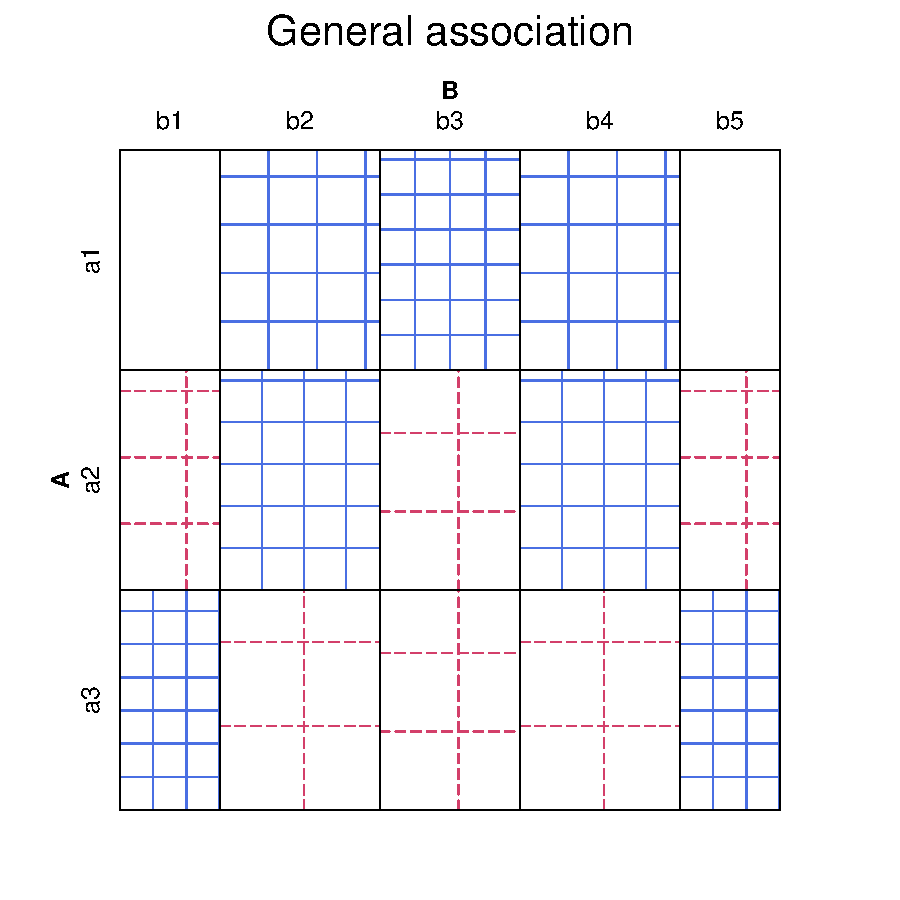
\includegraphics[width=.49\textwidth]{ch04/fig/cmhdemo-1} 
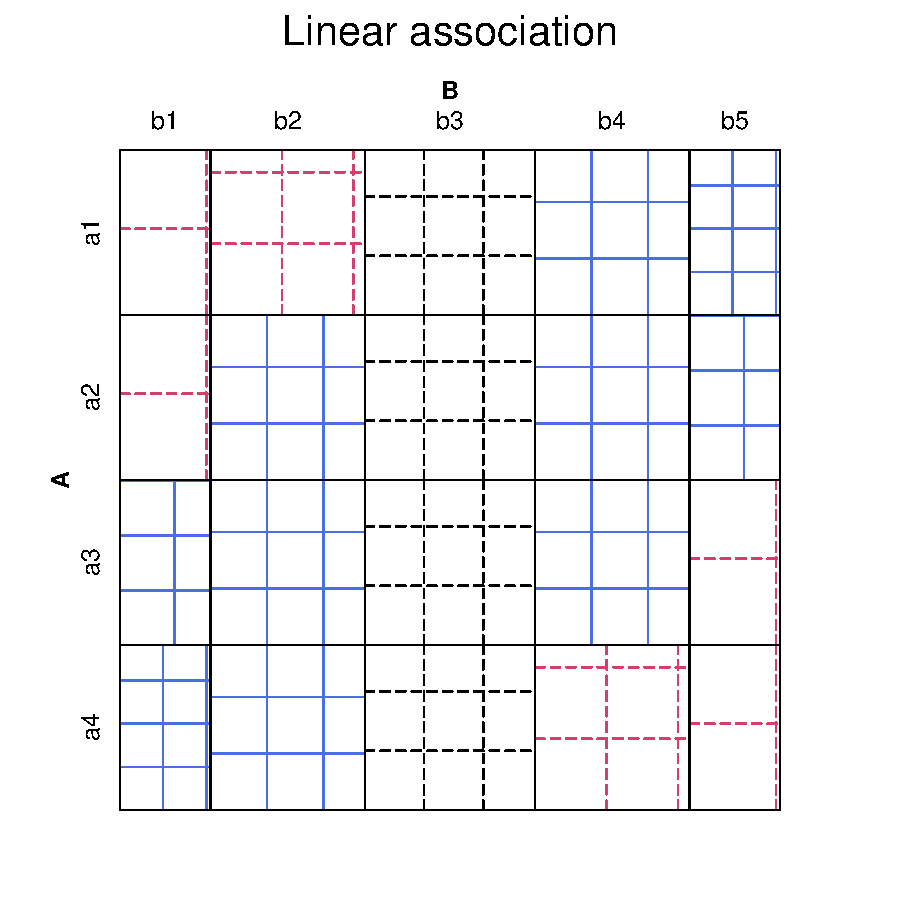
\includegraphics[width=.49\textwidth]{ch04/fig/cmhdemo-2} }

\caption[Sieve diagrams for two patterns of association]{Sieve diagrams for two patterns of association: Left: General association; right: Linear association\label{fig:cmhdemo}}
\end{figure}


\end{knitrout}

%<<cmhdemoprint,fig.keep="none">>=
%sieve(cmhdemo1, shade = TRUE, main = "General association")
%sieve(cmhdemo2, shade = TRUE, main = "Linear association")
%@

\subsubsection{Linear Association}

\ix{Cochran-Mantel-Haenszel tests!linear association}
The table below contains a weak,
non-significant general association, but significant row mean
differences and linear associations.
The unstructured test of general association would therefore
lead to the conclusion that no association exists, while the
tests taking ordinal factors into account would conclude otherwise.
Note that the largest frequencies
shift towards lower levels of $B$ as the level of variable $A$ increases.
See \figref{fig:cmhdemo} (right) for a visual representation of this pattern.

 \begin{center}
 \begin{tabular}{r|rrrrr|rr}
  \hline
     & b1 & b2 & b3 & b4 & b5 & Total & Mean \\ 
  \hline
  a1 & 2 & 5 & 8 & 8 & 8 & 31 & 3.48 \\ 
  a2 & 2 & 8 & 8 & 8 & 5 & 31 & 3.19 \\ 
  a3 & 5 & 8 & 8 & 8 & 2 & 31 & 2.81 \\ 
  a4 & 8 & 8 & 8 & 5 & 2 & 31 & 2.52 \\ 
  \hline
  Total & 17 & 29 & 32 & 29 & 17 & 124 & 3.00 \\ 
  Mean & 3.1 & 2.7 & 2.5 & 2.3 & 1.9 & 2.5\\
  \hline
 \end{tabular}
 \end{center}


Note that the \(\chi^2\)-values for the row-means and non-zero
correlation tests from \func{CMHtest}
are very similar, but the correlation test is more
highly significant since it is based on just one degree of
freedom. In the following example, \code{cmhdemo2} corresponds to the
table above:
\begin{knitrout}
\definecolor{shadecolor}{rgb}{1, 0.961, 0.933}\color{fgcolor}\begin{kframe}
\begin{alltt}
\hlstd{> }\hlkwd{CMHtest}\hlstd{(cmhdemo2)}
\end{alltt}
\begin{verbatim}
Cochran-Mantel-Haenszel Statistics 

                 AltHypothesis Chisq Df    Prob
cor        Nonzero correlation  10.6  1 0.00111
cmeans  Col mean scores differ  10.7  3 0.01361
rmeans  Row mean scores differ  11.4  4 0.02241
general    General association  13.4 12 0.34064
\end{verbatim}
\end{kframe}
\end{knitrout}
The difference in sensitivity and power among these tests
for categorical data is
analogous to the difference between general ANOVA tests and tests for
linear trend (contrasts)
in experimental designs with quantitative factors:
The more specific test has greater power, but is sensitive to
a narrower range of departures from the null hypothesis.
The more focused tests for ordinal factors are a better bet
when we believe that the association depends on the ordered
nature of the factor levels.

\section{Stratified analysis}\label{sec:twoway-strat}
An overall analysis ignores other variables (like sex), by
collapsing over them.  In the \data{Arthritis} data,
it is possible that the treatment is effective
only for one gender, or even that the treatment has opposite effects
for men and women.  If so, pooling over the ignored variable(s)
can be seriously misleading.
\ixd{arthritis treatment}

\subsection{Computing strata-wise statistics}\label{sec:twoway-strata}

A \term{stratified analysis} controls for the effects of one or more background variables.
This is similar to the use of a blocking variable in an ANOVA
design.  Tests for association can be obtained by applying
a function (\func{assocstats}, \func{CMHtest}) over the levels
of the stratifying variables.

\begin{comment}
\begin{itemize}

\item controls for the effects of one or more background variables.
       This is similar to the use of a blocking variable in an ANOVA
       design.

\item is obtained by including more than two variables in the {\tt
       tables} statement.  List the stratification variables {\bf
       first}.  To examine the association between TREAT and IMPROVE,
       controlling for both SEX and AGE (if available):

\begin{equation*}
   \mbox{\texttt{tables }}
   \overbrace{\rule{0in}{1.5ex}\mbox{\texttt{ age * sex }}}^{\mbox{\scriptsize stratify by}}
   \mbox{\texttt{ * }}
   \overbrace{\rule{0in}{1.5ex}\mbox{\texttt{ treat }}}^{\mbox{\scriptsize explanatory}}
   \mbox{\texttt{ * }}
   \overbrace{\rule{0in}{1.5ex}\mbox{\texttt{ improve;}}}^{\mbox{\scriptsize response}}
\end{equation*}
\end{itemize}
\end{comment}

\begin{Example}[arthrit3]{Arthritis treatment}
The statements below request a stratified analysis of the arthritis
treatment data
with CMH tests,
controlling for gender.  Essentially, the analysis is carried out
separately for males and females.

The table \code{Art2} is constructed as a three-way table,
with \var{Sex} as the last dimension.
\begin{knitrout}
\definecolor{shadecolor}{rgb}{1, 0.961, 0.933}\color{fgcolor}\begin{kframe}
\begin{alltt}
\hlstd{> }\hlstd{Art2} \hlkwb{<-} \hlkwd{xtabs}\hlstd{(}\hlopt{~} \hlstd{Treatment} \hlopt{+} \hlstd{Improved} \hlopt{+} \hlstd{Sex,} \hlkwc{data} \hlstd{= Arthritis)}
\hlstd{> }\hlstd{Art2}
\end{alltt}
\begin{verbatim}
, , Sex = Female

         Improved
Treatment None Some Marked
  Placebo   19    7      6
  Treated    6    5     16

, , Sex = Male

         Improved
Treatment None Some Marked
  Placebo   10    0      1
  Treated    7    2      5
\end{verbatim}
\end{kframe}
\end{knitrout}
\func{assocstats} only applies to two-way tables, so we use
\func{apply} to run it for each level of \var{Sex}.
\func{CMHtest} is designed for such stratified tables, and
uses all dimensions after the first two as strata.
\begin{knitrout}
\definecolor{shadecolor}{rgb}{1, 0.961, 0.933}\color{fgcolor}\begin{kframe}
\begin{alltt}
\hlstd{> }\hlkwd{apply}\hlstd{(Art2,} \hlkwc{MARGIN} \hlstd{=} \hlnum{3}\hlstd{,} \hlkwc{FUN} \hlstd{= assocstats)}
\end{alltt}
\begin{verbatim}
$Female
                    X^2 df  P(> X^2)
Likelihood Ratio 11.731  2 0.0028362
Pearson          11.296  2 0.0035242

Phi-Coefficient   : 0.438 
Contingency Coeff.: 0.401 
Cramer's V        : 0.438 

$Male
                    X^2 df P(> X^2)
Likelihood Ratio 5.8549  2 0.053532
Pearson          4.9067  2 0.086003

Phi-Coefficient   : 0.443 
Contingency Coeff.: 0.405 
Cramer's V        : 0.443 
\end{verbatim}
\end{kframe}
\end{knitrout}
Note that even though the strength of association ($\phi$-coefficient)
is similar in the two groups, the $\chi^2$ tests show
significance for females, but not for males.
This is true even using the more powerful CMH tests below, treating
\var{Treatment} as ordinal.  The reason is that there were more than
twice as many females as males in this sample.
\begin{knitrout}
\definecolor{shadecolor}{rgb}{1, 0.961, 0.933}\color{fgcolor}\begin{kframe}
\begin{alltt}
\hlstd{> }\hlkwd{CMHtest}\hlstd{(Art2)}
\end{alltt}
\begin{verbatim}
$`Sex:Female`
Cochran-Mantel-Haenszel Statistics for Treatment by Improved 
	in stratum Sex:Female 

                 AltHypothesis Chisq Df     Prob
cor        Nonzero correlation  10.9  1 0.000944
cmeans  Col mean scores differ  10.9  1 0.000944
rmeans  Row mean scores differ  11.1  2 0.003878
general    General association  11.1  2 0.003878


$`Sex:Male`
Cochran-Mantel-Haenszel Statistics for Treatment by Improved 
	in stratum Sex:Male 

                 AltHypothesis Chisq Df   Prob
cor        Nonzero correlation  3.71  1 0.0540
cmeans  Col mean scores differ  3.71  1 0.0540
rmeans  Row mean scores differ  4.71  2 0.0949
general    General association  4.71  2 0.0949
\end{verbatim}
\begin{alltt}
\hlstd{> }\hlkwd{apply}\hlstd{(Art2,} \hlnum{3}\hlstd{, sum)}
\end{alltt}
\begin{verbatim}
Female   Male 
    59     25 
\end{verbatim}
\end{kframe}
\end{knitrout}

\end{Example}

\subsection{Assessing homogeneity of association}\label{sec:twoway-homog}
In a stratified analysis
it is often  crucial to know if the association between the
primary table variables is the same over all strata.  For
\(2 \times  2 \times k\) tables this question reduces to whether the \IX{odds ratio} is
the same in all k strata. The \Rpackage{vcd} implements
Woolf's test \citep{Woolf:1995} in \verb|woolf_test()|
for this purpose.

For larger $n$-way tables,
this question is equivalent to testing whether the association
between the primary variables, $A$ and $B$, say, is the same for
all levels of the stratifying variables, $C$, $D$, $\dots$.


\begin{Example}[berkeley1a]{Berkeley admissions}
Here we illustrate the use of Woolf's test for the \data{UCBAdmissions} data.
The test is significant, indicating that the odds ratios cannot be considered
equal across departments.  We will see why when we visualize the data
by department in the next section.
\begin{knitrout}
\definecolor{shadecolor}{rgb}{1, 0.961, 0.933}\color{fgcolor}\begin{kframe}
\begin{alltt}
\hlstd{> }\hlkwd{woolf_test}\hlstd{(UCBAdmissions)}
\end{alltt}
\begin{verbatim}

	Woolf-test on Homogeneity of Odds Ratios (no 3-Way
	assoc.)

data:  UCBAdmissions
X-squared = 17.902, df = 5, p-value = 0.003072
\end{verbatim}
\end{kframe}
\end{knitrout}

\end{Example}
\begin{Example}[arthrit4]{Arthritis treatment}
For the arthritis data, homogeneity means 
% that there is no three-way
% Treatment * Improved * Sex association.  That is, 
the association
between treatment and outcome (\var{improve})
is the same for both men and women. Again, we are using
\func{woolf\_test} to test if this assumption holds.

\begin{knitrout}
\definecolor{shadecolor}{rgb}{1, 0.961, 0.933}\color{fgcolor}\begin{kframe}
\begin{alltt}
\hlstd{> }\hlkwd{woolf_test}\hlstd{(Art2)}
\end{alltt}
\begin{verbatim}

	Woolf-test on Homogeneity of Odds Ratios (no 3-Way
	assoc.)

data:  Art2
X-squared = 0.3181, df = 1, p-value = 0.5728
\end{verbatim}
\end{kframe}
\end{knitrout}

Even though we found in the CMH analysis above that the
association between \var{Treatment} and \var{Improved}
was stronger for females than males, the analysis using
\func{woolf\_test} is clearly non-significant, so we cannot
reject homogeneity of association.
\end{Example}

\subsubsection*{Remark}
As will be discussed later in the chapter on log-linear models, 
in the case of a 3-way table, the hypothesis of homogeneity of
association among three variables A, B and C can be stated as the
\term{loglinear model} of no three-way association,
$\llmthree{AB}{AC}{BC}$.
This notation (described in \secref{sec:loglin-counts})
lists only the high-order association
terms in a linear model for log frequency.

This hypothesis can be stated
as the \loglin\ model,
\begin{equation}\label{eq:STO2}
 \texttt{[SexTreatment] [SexImproved] [TreatmentImproved]}
 \period
\end{equation}

Such tests can be carried out most conveniently using
\func{loglm} in the \Rpackage{MASS}.  The model formula
uses the standard \R notation \verb|()^2| to specify all
terms of order 2.
\begin{knitrout}
\definecolor{shadecolor}{rgb}{1, 0.961, 0.933}\color{fgcolor}\begin{kframe}
\begin{alltt}
\hlstd{> }\hlkwd{library}\hlstd{(MASS)}
\hlstd{> }\hlkwd{loglm}\hlstd{(}\hlopt{~} \hlstd{(Treatment} \hlopt{+} \hlstd{Improved} \hlopt{+} \hlstd{Sex)} \hlopt{^} \hlnum{2}\hlstd{,} \hlkwc{data} \hlstd{= Art2)}
\end{alltt}
\begin{verbatim}
Call:
loglm(formula = ~(Treatment + Improved + Sex)^2, data = Art2)

Statistics:
                    X^2 df P(> X^2)
Likelihood Ratio 1.7037  2  0.42663
Pearson          1.1336  2  0.56735
\end{verbatim}
\end{kframe}
\end{knitrout}
\noindent Consistent with the Woolf test, the interaction terms are not significant.

\section{Fourfold display for 2 x 2 tables}\label{sec:twoway-fourfold}

\ixon{fourfold display}
The \boldital{fourfold display} is a special case of a
\term{radial diagram} (or ``polar area chart'')
%developed by Florence Nightingale
%\citeyear{Nightingale:1857}
designed for the display of $2 \times 2$ (or $2 \times 2 \times k$)
tables
\citep{Fienberg:75,Friendly:94b,Friendly:94c}.
In this display the frequency
\(n_{ij}\) in each cell of a fourfold table is shown by a quarter
circle, whose radius is proportional to \(\sqrt { n_{ij} }\), so the
area is proportional to the cell count.
The fourfold display
is similar to a pie chart in using segments of
a circle to show frequencies.  It
differs from a pie chart in that it keeps the
angles of the segments constant and varies the radius,
whereas the pie chart varies the angles and keeps the radius constant.

The main purpose of this display is to depict the sample odds ratio,
\(\hat{\theta} = (n_{11} /  n_{12} )
\div  (n_{21} /  n_{22} )\).
An association between the variables
(\(\theta \neq 1\)) is shown by the tendency of diagonally opposite
cells in one direction to differ in size from those in the opposite
direction, and the display uses color or shading to show this
direction.  Confidence rings for the observed \(\theta\) allow a
visual test of the hypothesis of independence,
 \(H_0 :  \theta  =  1\).  They have
the property that (in a standardized display) the rings for adjacent quadrants overlap \emph{iff}
the observed counts are consistent with the null hypothesis.

\begin{Example}[berkeley2]{Berkeley admissions}
\figref{fig:berk-fourfold1}(left) shows the basic, unstandardized
fourfold display for the
Berkeley admissions data (\tabref{tab:berk22}).
Here, the area of each quadrant is proportional to the cell frequency,
shown numerically in each corner.
The odds ratio is proportional to the product of the areas
shaded dark, divided by the product of the areas shaded light.
The sample odds ratio, Odds (Admit\(|\)Male) / Odds(Admit\(|\)Female) is
1.84 (see \exref{ex:berkeley1a})
indicating that males were nearly twice as likely to be admitted.

\begin{knitrout}
\definecolor{shadecolor}{rgb}{1, 0.961, 0.933}\color{fgcolor}\begin{kframe}
\begin{alltt}
\hlstd{> }\hlkwd{fourfold}\hlstd{(Berkeley,} \hlkwc{std} \hlstd{=} \hlstr{"ind.max"}\hlstd{)}   \hlcom{# unstandardized}
\hlstd{> }\hlkwd{fourfold}\hlstd{(Berkeley,} \hlkwc{margin} \hlstd{=} \hlnum{1}\hlstd{)}        \hlcom{# equating gender}
\end{alltt}
\end{kframe}\begin{figure}[!htbp]

\centerline{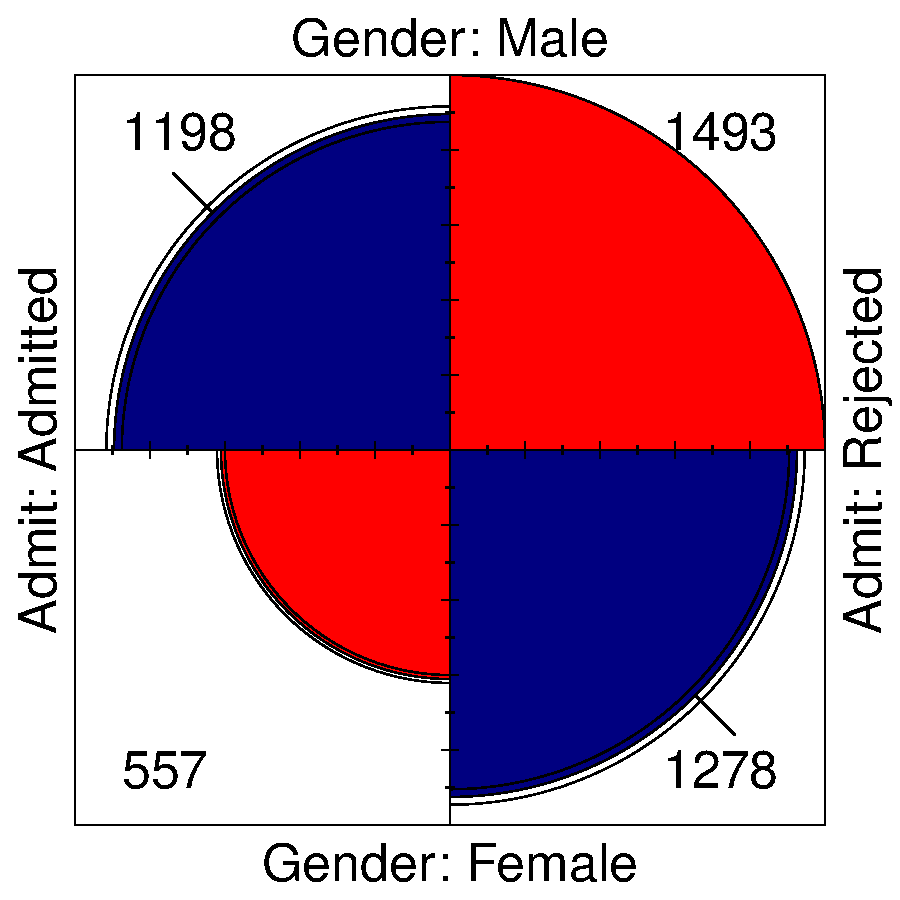
\includegraphics[width=.49\textwidth]{ch04/fig/berk-fourfold1-1} 
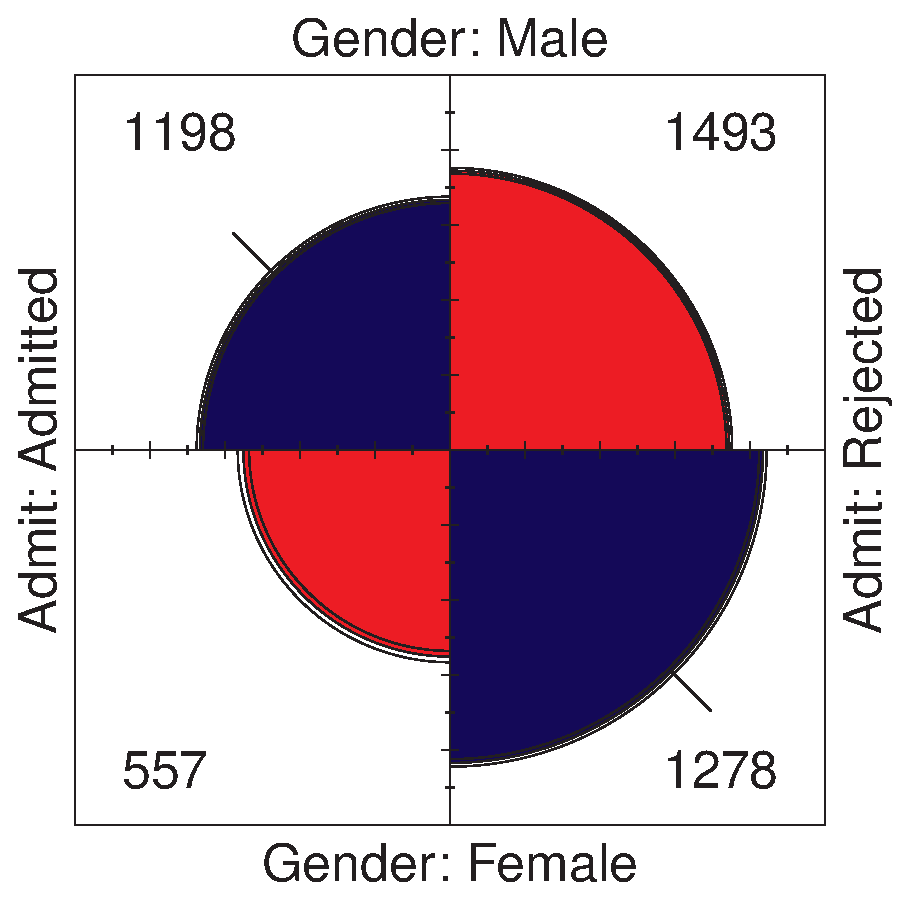
\includegraphics[width=.49\textwidth]{ch04/fig/berk-fourfold1-2} }

\caption[Fourfold displays for the Berkeley admission data]{Fourfold displays for the Berkeley admission data. Left: unstandardized; right: equating the proportions of males and females\label{fig:berk-fourfold1}}
\end{figure}


\end{knitrout}

However, it is difficult to make these visual comparisons
because there are more men than women, and because the
proportions admitted and rejected are unequal.  In the unstandardized
display the confidence bands have no interpretation as a test
of \(H_0 :  \theta  =  1\).

\begin{table}[htb]
\caption{Admissions to Berkeley graduate programs, Frequencies and Row Percentages}
\label{tab:berkrow}
 \begin{center}
\begin{tabular}{lrr|rr}
\hline
  & \multicolumn{2}{c|}{Frequencies} &\multicolumn{2}{c}{Row Percents} \\
  & Admitted & Rejected & Admitted & Rejected  \\
\hline
 Males  & 1198 & 1493 &  44.52 & 55.48  \\
 Females & 557 & 1278 &  30.35 & 69.65  \\
\hline
\end{tabular}
\end{center}
\end{table}

The data in a $2 \times 2$ table can be standardized to make these
visual comparisons easier.
\tabref{tab:berkrow} shows the Berkeley data with the addition of
row percentages (which equate for the number of men and women applicants)
 indicating the proportion of each gender accepted
and rejected.
We see that 44.52\% of males were admitted, while only 30.35\% of
females were admitted.
Moreover, the row percentages have the same odds ratio as the
raw data: $44.52 \times 69.65 / 30.35 \times 55.48 = 1.84$.
\figref{fig:berk-fourfold1}(right) shows the fourfold display where
the area of each quarter circle is proportional to these row
percentages.

With this standardization, the confidence rings have the property
that the confidence rings for each upper quadrant will overlap
with those for the quadrant below it if the
odds ratio does not differ from 1.0.
(Details of the calculation of confidence rings are described
in the next section.)
No similar statement can be made about the
corresponding left and right quadrants, however, because
the overall rate of admission has not been standardized.

As a final step, we can standardize the data so that \emph{both} table margins
are equal, while preserving the odds ratio.
Each quarter circle is then drawn to have an area
proportional to this standardized cell frequency.  This makes it
easier to see the association between admission and sex without being
influenced by the overall admission rate or the differential tendency
of males and females to apply.  With this standardization, the four
quadrants will align (overlap) horizontally and vertically
when the odds ratio is 1, regardless of the
marginal frequencies.  The fully standardized display, which is
usually the most useful form, is shown in \figref{fig:berk-fourfold3}.

\begin{knitrout}
\definecolor{shadecolor}{rgb}{1, 0.961, 0.933}\color{fgcolor}\begin{kframe}
\begin{alltt}
\hlstd{> }\hlkwd{fourfold}\hlstd{(Berkeley)}  \hlcom{# standardize both margins}
\end{alltt}
\end{kframe}\begin{figure}[!htbp]

\centerline{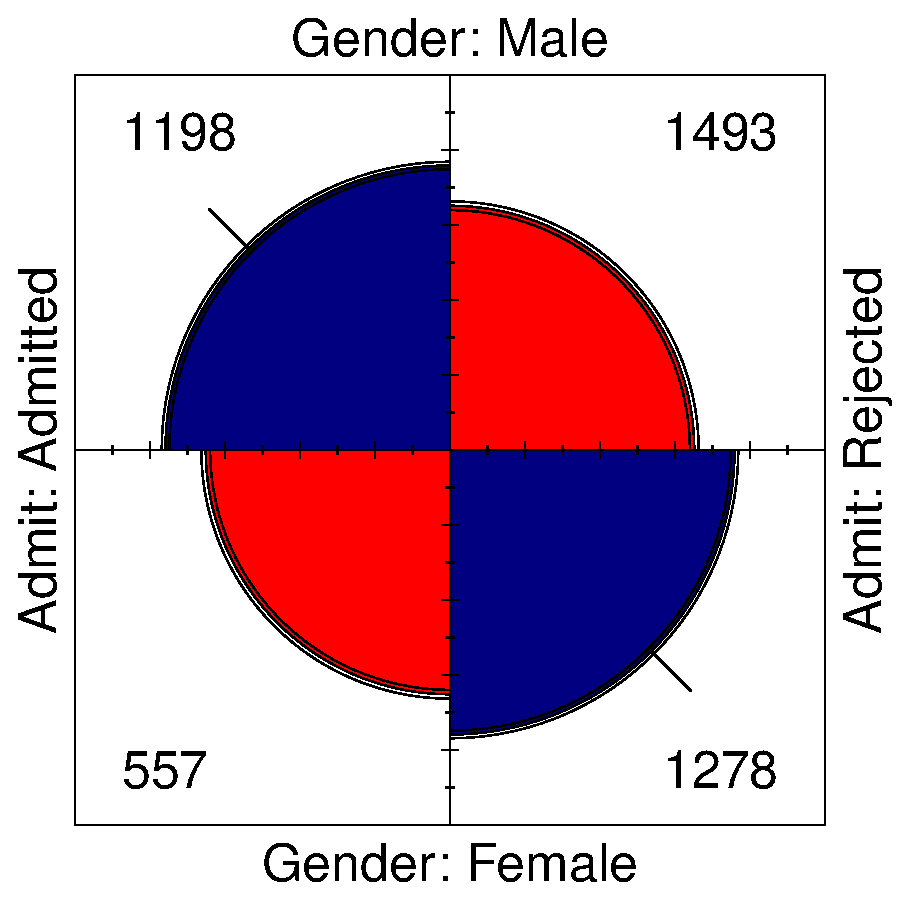
\includegraphics[width=.6\textwidth]{ch04/fig/berk-fourfold3-1} }

\caption[Fourfold display for Berkeley admission data with margins for gender and admission equated]{Fourfold display for Berkeley admission data with margins for gender and admission equated. The area of each quadrant shows the standardized frequency in each cell.\label{fig:berk-fourfold3}}
\end{figure}


\end{knitrout}

\end{Example}

These displays also use color (blue) and diagonal tick marks
to show the direction of positive association. The visual interpretation
(also conveyed by area) is that males are more likely to be accepted,
females more likely to be rejected.

The quadrants in \figref{fig:berk-fourfold3} do not align and
the 95\% confidence rings around each quadrant do not overlap,
indicating that the odds ratio differs significantly from 1---putative
evidence of gender bias.  The very narrow
width of the confidence rings gives a visual indication of the
precision of the data---if we stopped here, we might feel quite confident of this conclusion.

\subsection{Confidence rings for odds ratio}
\ixon{fourfold dislplay!confidence rings}
Confidence rings for the fourfold display are computed from a
confidence interval for \(\theta\), whose endpoints can each be
mapped into a \(2 \times  2\) table.  Each such table is then drawn
in the same way as the data.

The interval for \(\theta\) is most easily found by considering the
distribution of \(\hat{\psi}  =  \log  \hat{\theta} \), whose standard
error may be estimated by \eqref{eq:aselogtheta}.  Then an approximate \(1  -  \alpha\) confidence
interval for \(\psi\) is given by
\begin{equation*}
 \hat{\psi} \,\pm\,  \hat{s} ( \hat{\psi} )  \:
z_{ 1 - \alpha  / 2 } =  \{ \hat{\psi}_l , \,  \hat{\psi}_u \}
 \comma
\end{equation*}
as described in \secref{sec:twoway-twobytwo}.
The
corresponding limits for the odds ratio \(\theta\) are
\(\{ \exp ( \hat{\psi}_l ) , \,  \exp ( \hat{\psi}_u ) \}\).  For the data
shown in \figref{fig:berk-fourfold3},
\(\hat{\psi}  =  \log \,  \hat{\theta} =  .6104\),
and \(\hat{s}  ( \hat{\psi} )  =  0.0639\), so the 95\%,
limits for \(\theta\) are \(\{ 1.624, \,  2.087 \}\),
as shown by the calculations below. The same result is returned by \func{confint} for an
\class{oddsratio} object.
\begin{knitrout}
\definecolor{shadecolor}{rgb}{1, 0.961, 0.933}\color{fgcolor}\begin{kframe}
\begin{alltt}
\hlstd{> }\hlkwd{summary}\hlstd{(}\hlkwd{oddsratio}\hlstd{(Berkeley))}
\end{alltt}
\begin{verbatim}
     Log Odds Ratio Std. Error z value Pr(>|z|)    
[1,]         0.6104     0.0639    9.55   <2e-16 ***
---
Signif. codes:  0 '***' 0.001 '**' 0.01 '*' 0.05 '.' 0.1 ' ' 1
\end{verbatim}
\begin{alltt}
\hlstd{> }\hlkwd{exp}\hlstd{(}\hlnum{.6103} \hlopt{+} \hlkwd{c}\hlstd{(}\hlopt{-}\hlnum{1}\hlstd{,} \hlnum{1}\hlstd{)} \hlopt{*} \hlkwd{qnorm}\hlstd{(}\hlnum{.975}\hlstd{)} \hlopt{*} \hlnum{0.06398}\hlstd{)}
\end{alltt}
\begin{verbatim}
[1] 1.6240 2.0869
\end{verbatim}
\begin{alltt}
\hlstd{> }\hlkwd{confint}\hlstd{(}\hlkwd{oddsratio}\hlstd{(Berkeley,} \hlkwc{log} \hlstd{=} \hlnum{FALSE}\hlstd{))}
\end{alltt}
\begin{verbatim}
        lwr    upr
[1,] 1.6244 2.0867
\end{verbatim}
\end{kframe}
\end{knitrout}

Now consider how to find a \(2 \times  2\) table whose frequencies
correspond to the odds ratios at the limits of the confidence
interval.  A table standardized to equal row and column margins can
be represented by the \(2 \times  2\) matrix with entries
\begin{equation*}
 \left[
  \begin{array}{cc}
   p & (1-p) \\
  (1-p) & p
  \end{array}
 \right]
 \comma
\end{equation*}
whose odds ratio is \(\theta  =  p^2 /  ( 1  -  p)^2\).
Solving for $p$ gives \(p  =  \sqrt \theta /  ( 1  +  \sqrt \theta )\).  The
corresponding frequencies can then be found by adjusting the
standardized table to have the same row and column margins as the
data. The results of these computations which generate the confidence
rings in \figref{fig:berk-fourfold3} are shown in \tabref{tab:berkodds}.
%\DONE{Re-calculate this table for $\alpha=0.05$}

\begin{table}[htb]
\caption{Odds ratios and equivalent tables for confidence rings.}\label{tab:berkodds}
 \begin{center}
\begin{tabular}{lr|rr|rr}
\hline
   &      Odds    & \multicolumn{2}{c|}{Standardized} & \multicolumn{2}{c}{Equivalent}  \\
   &      Ratio   & \multicolumn{2}{c|}{Table}   &  \multicolumn{2}{c}{Frequencies} \\
\hline
Lower &   1.562   &    0.555 & 0.445   &  1157.2 &  1533.8 \\
limit &           &    0.445 & 0.555   &   597.8 &  1237.2 \\[2ex]

Data  &   1.841   &    0.576 & 0.424   &  1198.0 &  1493.0 \\
      &           &    0.424 & 0.576   &   557.0 &  1278.0 \\[2ex]

Upper &   2.170   &    0.596 & 0.404   &  1237.8 &  1453.2 \\
limit &           &    0.404 & 0.596   &   517.2 &  1317.8 \\
\hline
\end{tabular}
\end{center}
\end{table}

\ixoff{fourfold dislplay!confidence rings}

% \subsection{\func{fourfold} details}
% \TODO{Is this necessary?}

\subsection{Stratified analysis for $2 \times 2 \times k$ tables}\label{sec:twoway-fourstrat}
In a \(2 \times  2 \times  k\)
table, the last dimension often corresponds to ``strata'' or
populations, and it is typically of interest to see if the
association between the first two variables is homogeneous across
strata.  For such tables, simply make one fourfold panel for each
stratum.  The standardization of marginal frequencies is designed to
allow easy visual comparison of the pattern of association
when the marginal frequencies vary across two
or more populations.

\subsubsection{Stratified displays}\label{sec:twoway-strat}

The admissions data shown in
\figref{fig:berk-fourfold1} and \figref{fig:berk-fourfold3} were actually obtained
from six departments---the six largest at Berkeley
\citep{Bickel-etal:75}.
To determine the source of the apparent sex
bias in favor of males, we make a new plot, \figref{fig:berk-fourfold4},
stratified by department.
\ixd{Berkeley admissions}

\begin{knitrout}
\definecolor{shadecolor}{rgb}{1, 0.961, 0.933}\color{fgcolor}\begin{kframe}
\begin{alltt}
\hlstd{> }\hlcom{# fourfold display}
\hlstd{> }\hlstd{UCB} \hlkwb{<-} \hlkwd{aperm}\hlstd{(UCBAdmissions,} \hlkwd{c}\hlstd{(}\hlnum{2}\hlstd{,} \hlnum{1}\hlstd{,} \hlnum{3}\hlstd{))}
\hlstd{> }\hlkwd{fourfold}\hlstd{(UCB,} \hlkwc{mfrow} \hlstd{=} \hlkwd{c}\hlstd{(}\hlnum{2}\hlstd{,} \hlnum{3}\hlstd{))}
\end{alltt}
\end{kframe}\begin{figure}[!htbp]

\centerline{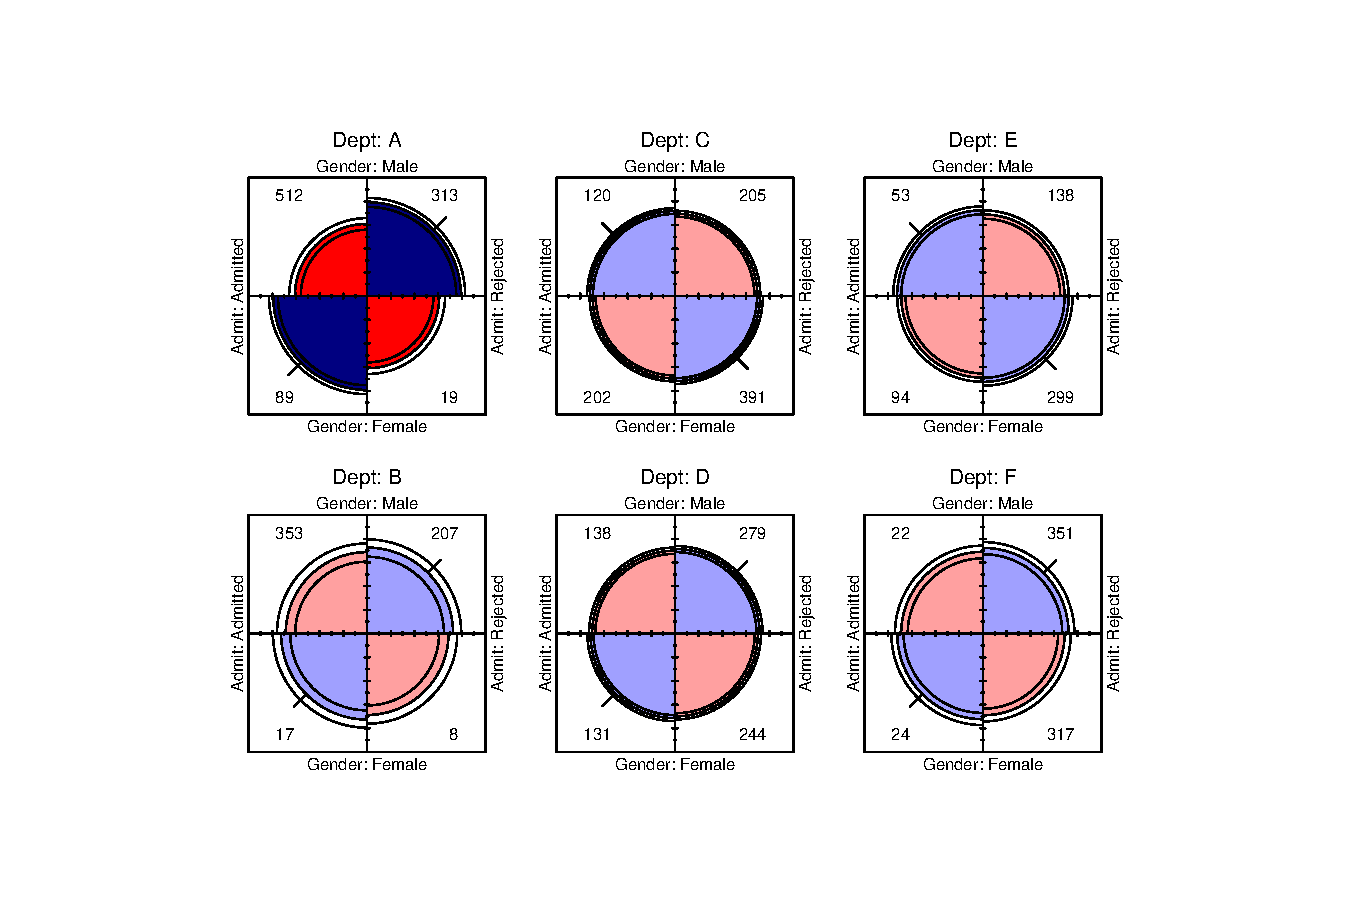
\includegraphics[width=.95\textwidth,trim=80 50 80 50]{ch04/fig/berk-fourfold4-1} }

\caption[Fourfold displays for Berkeley admissions data, stratified by department]{Fourfold displays for Berkeley admissions data, stratified by department. The more intense shading for Dept. A indicates a significant association.\label{fig:berk-fourfold4}}
\end{figure}


\end{knitrout}
% \TODO{Figure out how to trim these grid figures. Here, I'm
% using \code{out.extra='trim= ...'}, but maybe pdfcrop is easier. }

Surprisingly, \figref{fig:berk-fourfold4} shows that, for five of the
six departments, the odds of admission is approximately the same for
both men and women applicants.  Department A appears to differs from
the others, with women approximately 2.86 (\(=  ( 313/19 )  /
(512/89)\)) times as likely to gain admission.  This appearance is
confirmed by the confidence rings, which in \figref{fig:berk-fourfold4}
are joint%
\footnote{
For multiple-strata plots, \func{fourfold} by default adjusts the
significance level for multiple testing, using Holm's
\citeyearpar{Holm:1979} method
provided by \func{p.adjust}.
}
95\% intervals for \(\theta_c ,  \,  c = 1, \dots ,
k\).

This result, which contradicts the display for the aggregate data in
\figref{fig:berk-fourfold1}, is a nice example of
\term{Simpson's paradox}%
\footnote{Simpson's paradox \citep{Simpson:51} occurs in a three-way
table, $[A, B, C]$, when the marginal association between two variables,
$A, B$ collapsing over $C$ differs in \emph{direction} from the partial
association $A, B | C= c_k$ at the separate levels of $C$.
Strictly speaking, Simpson's paradox would require that for all
departments separately the odds ratio $\theta_k < 1$
(which occurs for Departments A, B, D, and F in \figref{fig:berk-fourfold4})
while in the aggregate data $\theta > 1$.
},
and illustrates clearly why an overall analysis of a three- (or higher-)
way table can be misleading.
\ix{Simpson's paradox}
The resolution of this contradiction can be found in the large
differences in admission rates among departments.  Men and women
apply to different departments differentially, and in these data
women happen to apply in larger numbers to departments that have a low
acceptance rate.  The aggregate results are misleading because they
falsely assume men and women are equally likely to apply in each
field.\footnote{This explanation ignores the possibility of structural bias
against women, e.g.,\ lack of resources allocated to departments that
attract women applicants.}

\subsubsection{Visualization principles for complex data}
\TODO{Move this to Ch. 1}
An important principle in the display of large, complex data sets
is \term{controlled comparison}---we want to make comparisons
against a clear standard, with
other things held constant.
The fourfold display
differs from a pie chart in that it holds the
angles of the segments constant and varies the radius.
An important consequence is that we can quite easily compare a
series of fourfold displays for different strata, since corresponding
cells of the table are always in the same position.
As a result, an array of fourfold displays serve the goals of comparison and
detection better than an array of pie charts.

Moreover, it allows the observed frequencies to be standardized
by equating either the row or column totals, while preserving
the design goal for this display---the odds ratio.
In \figref{fig:berk-fourfold4}, for example,
the proportion of men and women, and the proportion
of accepted applicants were equated visually in each department.
This provides a clear standard which
also greatly facilitates controlled comparison.

Another principle is \term{visual impact}---we want the important
features
of the display to be easily distinguished from the less important
\citep{Tukey:93}.
\figref{fig:berk-fourfold4} distinguishes the one department for which
the odds ratio differs significantly from 1 by shading intensity,
even though the same information can be found by inspection of the
confidence rings.

\begin{Example}[wheeze1]{Breathlessness and wheeze in coal miners}
The various ways of standardizing a collection of $2 \times 2$ tables
allows visualizing relations with different factors
(row percentages, column percentages, strata totals) controlled.
However, different kinds of graphs can speak more eloquently to other questions by focusing more directly on the odds ratio.

\citet[Table 9.8]{Agresti:2002} cites data from
\citet{AshfordSowden:70} on the association between
two pulmonary conditions, breathlessness and wheeze, in a large sample of coal miners.
The miners are classified into age groups, and the question treated
by Agresti is whether the association between these two symptoms
is homogeneous over age.%
These data are available in the \data{CoalMiners} data in
\pkg{vcd}, a $2 \times 2 \times 9$ frequency table.
The first group, aged 20--24 has been omitted from these
analyses.
\begin{knitrout}
\definecolor{shadecolor}{rgb}{1, 0.961, 0.933}\color{fgcolor}\begin{kframe}
\begin{alltt}
\hlstd{> }\hlkwd{data}\hlstd{(}\hlstr{"CoalMiners"}\hlstd{,} \hlkwc{package} \hlstd{=} \hlstr{"vcd"}\hlstd{)}
\hlstd{> }\hlstd{CM} \hlkwb{<-} \hlstd{CoalMiners[, ,} \hlnum{2} \hlopt{:} \hlnum{9}\hlstd{]}
\hlstd{> }\hlkwd{structable}\hlstd{(.} \hlopt{~} \hlstd{Age,} \hlkwc{data} \hlstd{= CM)}
\end{alltt}
\begin{verbatim}
      Breathlessness    B       NoB     
      Wheeze            W  NoW    W  NoW
Age                                     
25-29                  23    9  105 1654
30-34                  54   19  177 1863
35-39                 121   48  257 2357
40-44                 169   54  273 1778
45-49                 269   88  324 1712
50-54                 404  117  245 1324
55-59                 406  152  225  967
60-64                 372  106  132  526
\end{verbatim}
\end{kframe}
\end{knitrout}

The question of interest
can be addressed by displaying the odds ratio
in the $2 \times 2$ tables with the margins of breathlessness
and wheeze equated (i.e., with the default \code{std='margins'} option),
which gives the graph shown in \figref{fig:coalminer1}.
Although the panels for all age groups show an overwhelmingly
positive association between these two symptoms, one can also
(by looking carefully)
see that the strength of this association declines with increasing
age.

\begin{knitrout}
\definecolor{shadecolor}{rgb}{1, 0.961, 0.933}\color{fgcolor}\begin{kframe}
\begin{alltt}
\hlstd{> }\hlkwd{fourfold}\hlstd{(CM,} \hlkwc{mfcol} \hlstd{=} \hlkwd{c}\hlstd{(}\hlnum{2}\hlstd{,} \hlnum{4}\hlstd{))}
\end{alltt}
\end{kframe}\begin{figure}[!htbp]

\centerline{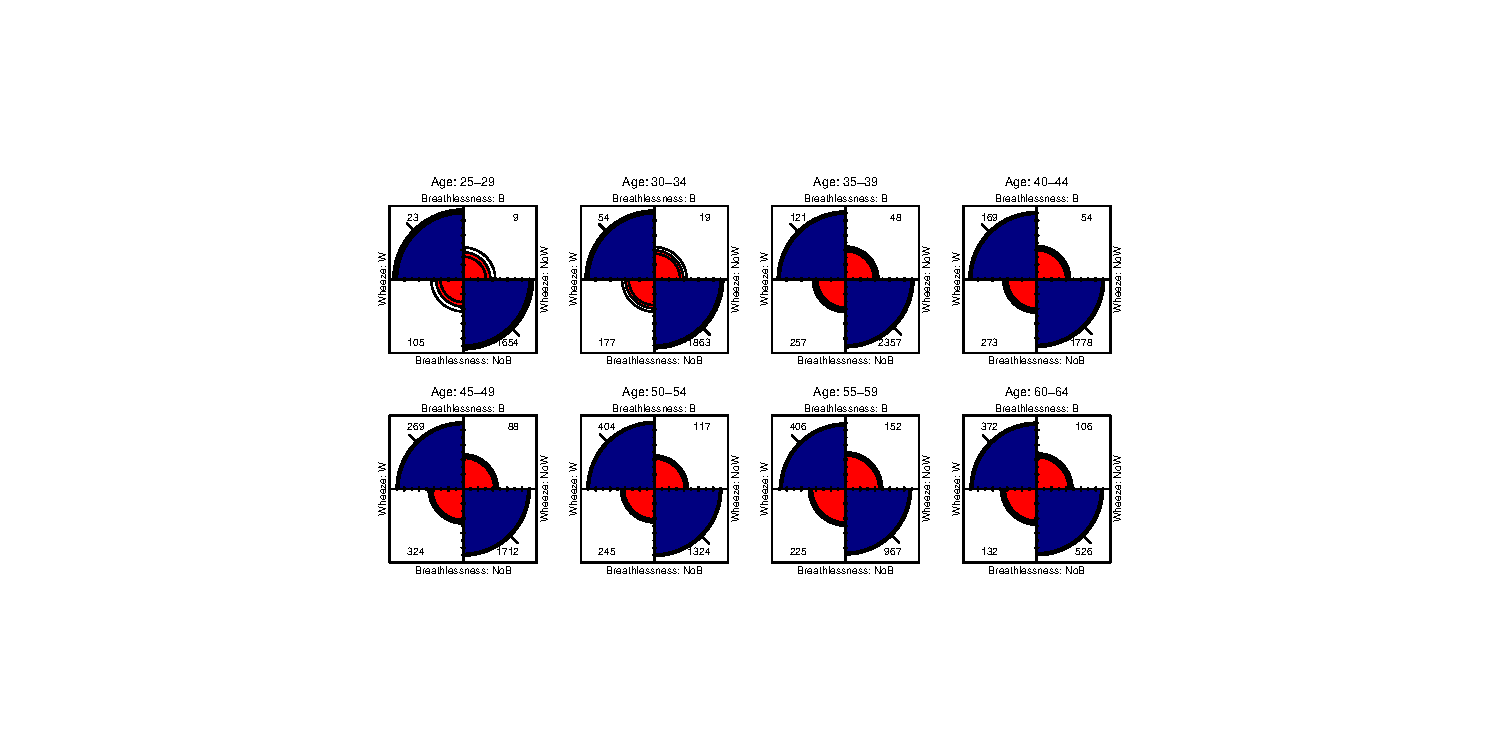
\includegraphics[width=\textwidth,trim=120 80 120 80]{ch04/fig/coalminer1-1} }

\caption[Fourfold display for CoalMiners data, both margins equated]{Fourfold display for CoalMiners data, both margins equated\label{fig:coalminer1}}
\end{figure}


\end{knitrout}

However, note that the pattern of change over age is somewhat subtle
compared to the dominant positive association within each
panel.
When the goal is to display how the odds ratio varies with
a quantitative factor such as age, it is often better to simply
calculate and plot the odds ratio directly.
%, as shown in \figref{fig:pie2x2wh2}.

The \func{oddsratio} function in \pkg{vcd} calculates odds ratios
for $2 \times 2 (\times k)$ tables.  By default, it returns the
log odds.  Use the option \code{log=FALSE} to get the odds ratios
themselves.  It is easy to see that the (log) odds ratios decline
with age.
\begin{knitrout}
\definecolor{shadecolor}{rgb}{1, 0.961, 0.933}\color{fgcolor}\begin{kframe}
\begin{alltt}
\hlstd{> }\hlkwd{oddsratio}\hlstd{(CM)}
\end{alltt}
\begin{verbatim}
 25-29  30-34  35-39  40-44  45-49  50-54  55-59  60-64 
3.6953 3.3983 3.1407 3.0147 2.7820 2.9264 2.4406 2.6380 
\end{verbatim}
\begin{alltt}
\hlstd{> }\hlkwd{oddsratio}\hlstd{(CM,} \hlkwc{log} \hlstd{=} \hlnum{FALSE}\hlstd{)}
\end{alltt}
\begin{verbatim}
 25-29  30-34  35-39  40-44  45-49  50-54  55-59  60-64 
40.256 29.914 23.119 20.383 16.152 18.660 11.480 13.985 
\end{verbatim}
\end{kframe}
\end{knitrout}
When the analysis goal is to understand how the odds ratio varies
with a stratifying factor (which could be a quantitative variable),
it is often better to plot the odds ratio directly.

The lines below
use the \func{plot} method for \class{oddsratio} objects.
This produces a line graph of the log odds ratio against the
stratum variable, together with confidence interval error bars.
In addition, because age is a quantitative variable, we can
calculate, and display the fitted relation for a linear model
relating \code{lodds} to \code{age}.  Here, we try using a
quadratic model (\code{poly(age, 2)}) mainly to see if the
trend is nonlinear.
\begin{knitrout}
\definecolor{shadecolor}{rgb}{1, 0.961, 0.933}\color{fgcolor}\begin{kframe}
\begin{alltt}
\hlstd{> }\hlstd{lodds} \hlkwb{<-} \hlkwd{oddsratio}\hlstd{(CM)}
\hlstd{> }\hlkwd{plot}\hlstd{(lodds,} \hlkwc{lwd} \hlstd{=} \hlnum{2}\hlstd{,} \hlkwc{cex} \hlstd{=} \hlnum{1.25}\hlstd{,} \hlkwc{pch} \hlstd{=} \hlnum{16}\hlstd{,}
\hlstd{+ }     \hlkwc{xlab} \hlstd{=} \hlstr{"Age Group"}\hlstd{,}
\hlstd{+ }     \hlkwc{main} \hlstd{=} \hlstr{"Breathlessness and Wheeze in Coal Miners"}\hlstd{)}
\hlstd{> }\hlstd{age} \hlkwb{<-} \hlkwd{seq}\hlstd{(}\hlnum{25}\hlstd{,} \hlnum{60}\hlstd{,} \hlkwc{by} \hlstd{=} \hlnum{5}\hlstd{)} \hlopt{+} \hlnum{2}
\hlstd{> }\hlstd{mod} \hlkwb{<-} \hlkwd{lm}\hlstd{(lodds} \hlopt{~} \hlkwd{poly}\hlstd{(age,} \hlnum{2}\hlstd{))}
\hlstd{> }\hlkwd{lines}\hlstd{(}\hlkwd{fitted}\hlstd{(mod),} \hlkwc{col} \hlstd{=} \hlstr{"red"}\hlstd{,} \hlkwc{lwd} \hlstd{=} \hlnum{2}\hlstd{)}
\end{alltt}
\end{kframe}\begin{figure}[!htbp]

\centerline{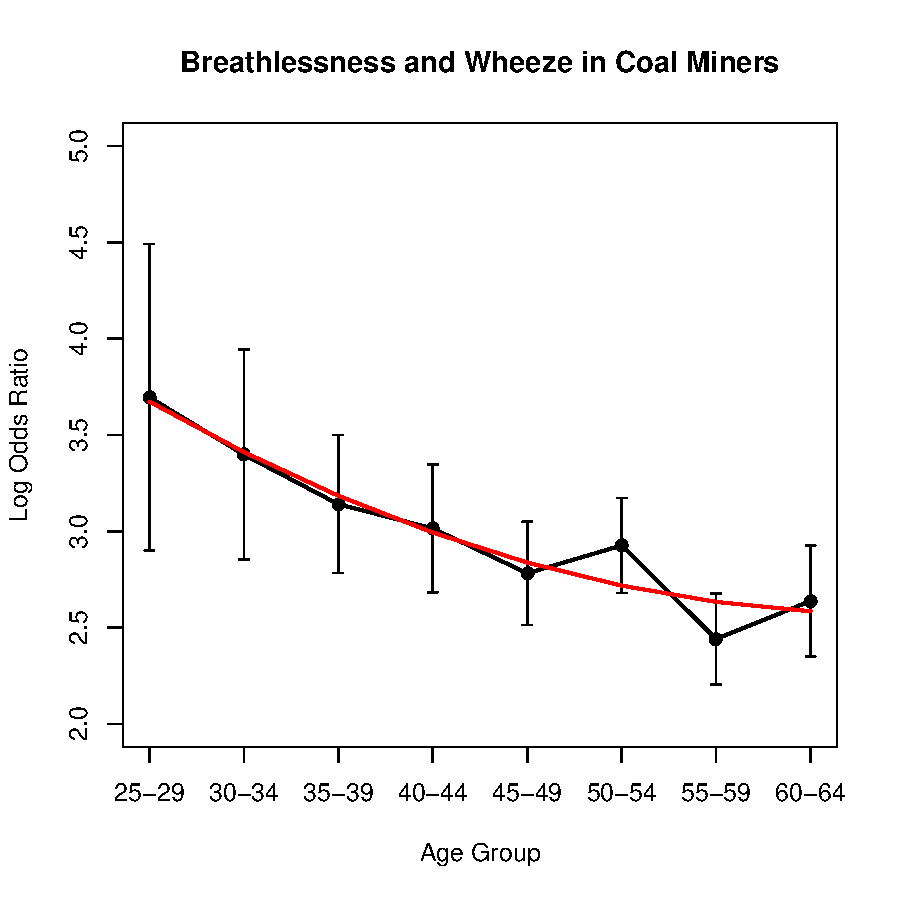
\includegraphics[width=.6\textwidth]{ch04/fig/coalminer3-1} }

\caption[Log odds plot for the CoalMiners data]{Log odds plot for the CoalMiners data.  The smooth curve shows a quadratic fit to age.\label{fig:coalminer3}}
\end{figure}


\end{knitrout}
In \figref{fig:coalminer3}, it appears that the decline in the
log odds ratio levels off with increasing age.  One virtue of
fitting the model in this way is that we can test the additional contribution
of the quadratic term, which turns out to be insignificant.
\begin{knitrout}
\definecolor{shadecolor}{rgb}{1, 0.961, 0.933}\color{fgcolor}\begin{kframe}
\begin{alltt}
\hlstd{> }\hlkwd{summary}\hlstd{(mod)}
\end{alltt}
\begin{verbatim}

Call:
lm(formula = lodds ~ poly(age, 2))

Residuals:
  25-29   30-34   35-39   40-44   45-49   50-54   55-59   60-64 
 0.0219 -0.0128 -0.0438  0.0213 -0.0558  0.2085 -0.1928  0.0534 

Coefficients:
              Estimate Std. Error t value Pr(>|t|)    
(Intercept)     3.0045     0.0473   63.46  1.8e-08 ***
poly(age, 2)1  -1.0080     0.1339   -7.53  0.00066 ***
poly(age, 2)2   0.2304     0.1339    1.72  0.14594    
---
Signif. codes:  0 '***' 0.001 '**' 0.01 '*' 0.05 '.' 0.1 ' ' 1

Residual standard error: 0.134 on 5 degrees of freedom
Multiple R-squared:  0.923,	Adjusted R-squared:  0.892 
F-statistic: 29.8 on 2 and 5 DF,  p-value: 0.00167
\end{verbatim}
\end{kframe}
\end{knitrout}

\end{Example}
\ixoff{fourfold display}

\section{Sieve diagrams}\label{sec:twoway-sieve}

\ixon{sieve diagram}
%\epigraph{They consider me to have sharp and penetrating vision because I see them through the mesh of a sieve.}{Kahlil Gibran}
\epigraph{The wise ones fashioned speech with their thought, sifting it as grain is sifted through a sieve.}{Buddha}
For two- (and higher-) way \ctabs, the
design principles of
perception, detection, and comparison
(see \chref{ch:intro})
suggest that we should try to show the observed frequencies
in relation to what we would expect those frequencies to be
under a reasonable null model---for example, the
hypothesis that the row and column variables are unassociated.

To this end, several schemes for representing \ctabs\
graphically are
based on the fact that when the row and column variables are
independent, the estimated expected frequencies, \(m_{ij}\), are
products of the row and column totals (divided by the grand total).
\begin{equation*}
 m_{ij} = \frac{ n_{i+} n_{+j} } { n_{++} }
 \period
\end{equation*}
Then, each cell can be represented by a rectangle whose area shows
the observed cell frequency, \(n_{ij}\),  expected frequency, \(m_{ij}\),
or deviation (residual) from independence, \(n_{ij} - m_{ij}\).
Visual attributes (color, shading) of the rectangles can be used to
highlight the pattern of association.

\subsection{Two-way tables}\label{sec:twoway-sieve}

For example, for any two-way table, the expected frequencies under independence
can be represented by rectangles whose widths are proportional to the
total frequency in each column, \(n_{+j}\), and whose heights are
proportional to the total frequency in each row, \(n_{i+}\); the area
of each rectangle is then proportional to \(m_{ij}\). \figref{fig:HE-sieve} (left)
shows the expected frequencies for the hair and eye color
data (\tabref{tab:hairdat}), calculated using
\func{independence\_table} in \pkg{vcd}.
\begin{knitrout}
\definecolor{shadecolor}{rgb}{1, 0.961, 0.933}\color{fgcolor}\begin{kframe}
\begin{alltt}
\hlstd{> }\hlstd{haireye} \hlkwb{<-} \hlkwd{margin.table}\hlstd{(HairEyeColor,} \hlnum{1}\hlopt{:}\hlnum{2}\hlstd{)}
\hlstd{> }\hlstd{expected} \hlkwb{=} \hlkwd{independence_table}\hlstd{(haireye)}
\hlstd{> }\hlkwd{round}\hlstd{(expected,} \hlnum{1}\hlstd{)}
\end{alltt}
\begin{verbatim}
       Eye
Hair    Brown  Blue Hazel Green
  Black  40.1  39.2  17.0  11.7
  Brown 106.3 103.9  44.9  30.9
  Red    26.4  25.8  11.2   7.7
  Blond  47.2  46.1  20.0  13.7
\end{verbatim}
\end{kframe}
\end{knitrout}



\begin{knitrout}
\definecolor{shadecolor}{rgb}{1, 0.961, 0.933}\color{fgcolor}\begin{figure}[!htbp]

\centerline{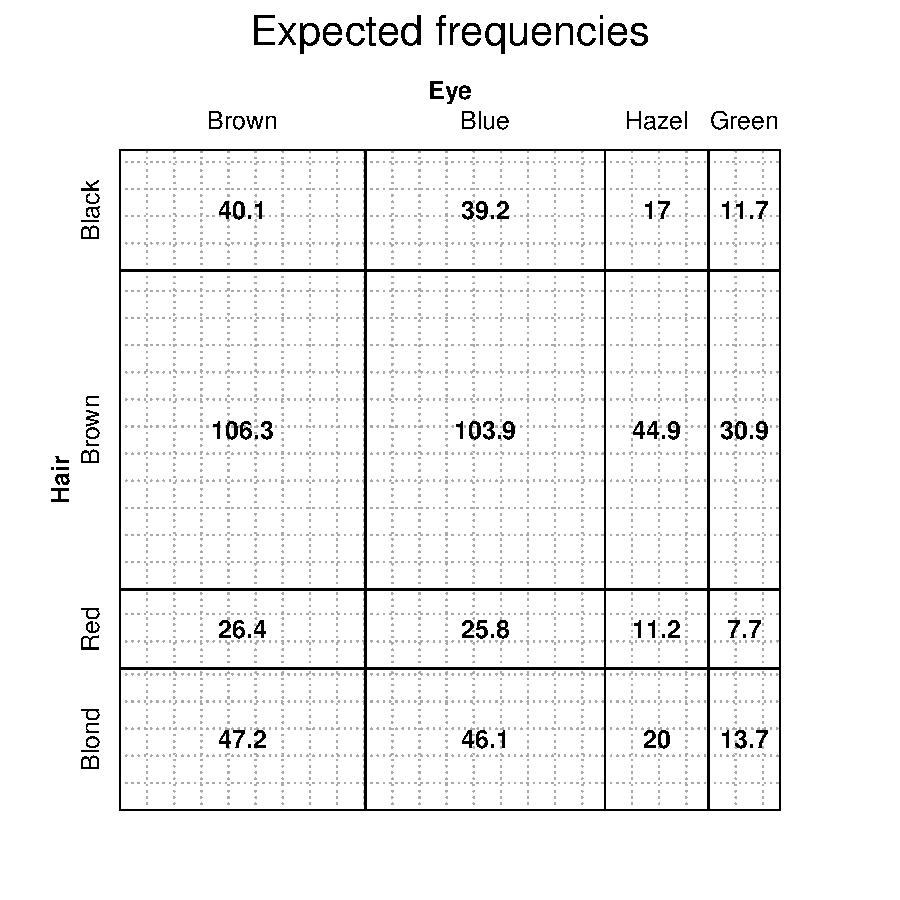
\includegraphics[width=.49\textwidth]{ch04/fig/HE-sieve-1} 
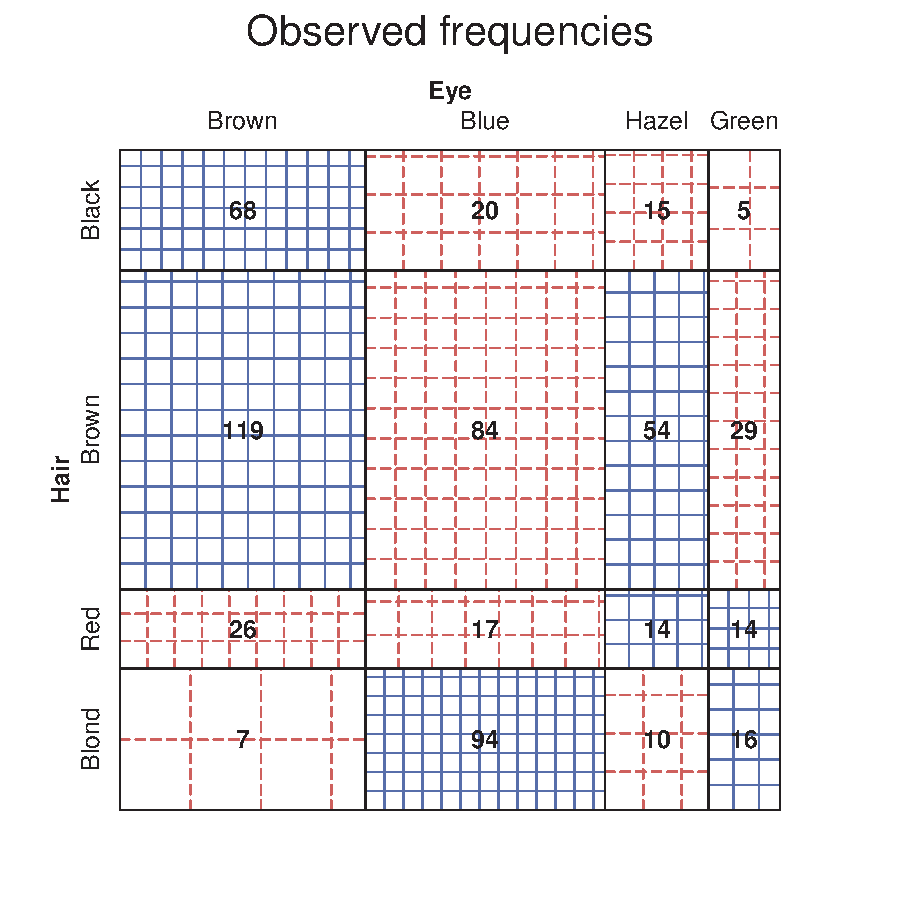
\includegraphics[width=.49\textwidth]{ch04/fig/HE-sieve-2} }

\caption[Sieve diagrams for the \data{HairEyeColor} data]{Sieve diagrams for the \data{HairEyeColor} data. Left: expected frequencies shown in cells as numbers and the number of boxes; right: observed frequencies shown in cells.\label{fig:HE-sieve}}
\end{figure}


\end{knitrout}

\figref{fig:HE-sieve} (left) simply represents the model---what the frequencies would
be if hair color and eye color were independent---not the data.
Note, however, that the rectangles are cross-ruled so that the number of
boxes in each (counting up the fractional bits) equals the expected
frequency with which the cell is labeled, and moreover, the
rulings are equally spaced in all cells.
Hence, cross-ruling the cells to show the observed frequency
would give a data display which implicitly compares observed
and expected frequencies as shown in \figref{fig:HE-sieve} (right).


Riedwyl and Sch\"{u}pbach (\citeyear{RiedwylSchupbach:83,RiedwylSchupbach:94})
proposed a
\term{sieve diagram}
(later called a \term{parquet diagram}) based on
this principle.  In this display the area of each rectangle is
always proportional to expected frequency
but observed frequency is shown by
the number of squares in each rectangle,
as in \figref{fig:HE-sieve} (right).

Hence, the difference
between observed and expected frequency appears as variations in the density of
shading.
Cells whose observed frequency $n_{ij}$ exceeds the expected $m_{ij}$
appear denser than average.
The pattern of positive and negative deviations from independence
can be more easily seen by
using color, say, red for negative deviations, and blue for positive.%
\footnote{
Positive residuals are also shown by solid lines, negative residuals by broken
lines, so that they may still be distinguished in monochrome versions.}

\begin{Example}[haireye2]{Hair color and eye color}
The sieve diagram for hair color and eye color
shown in
\figref{fig:HE-sieve} (right) can be interpreted as follows:
The pattern of color and shading shows the high frequency of
blue-eyed blonds and people with brown eyes and dark hair.
People with hazel eyes are also more likely to have red or brown hair,
and those with green eyes more likely to have red or blond hair,
than would be observed under independence.
\end{Example}

\begin{Example}[vision1]{Visual acuity}
In World War II, all workers in the U.K. Royal Ordnance factories
were given test of visual acuity (unaided distance vision)
of their left and right eyes
on a 1 (high) to 4 (low) scale.  The dataset \data{VisualAcuity}
in \pkg{vcd} gives the results for 10,719 workers
(3,242 men, 7,477 women) aged 30--39.

\figref{fig:VA-sieve2} shows the sieve diagram for data
from the larger sample of women
(\citet[Table 33.5]{KendallStuart:61},
\citet[p. 284]{Bishop-etal:75}).
The \data{VisualAcuity} data is a frequency data frame
and we first convert it to table form (\code{VA}),
a $4 \times 4 \times 2$
table to re-label the variables and levels.
%\DONE{Make this an exercise in Ch. 2}
\begin{knitrout}
\definecolor{shadecolor}{rgb}{1, 0.961, 0.933}\color{fgcolor}\begin{kframe}
\begin{alltt}
\hlstd{> }\hlcom{# re-assign names/dimnames}
\hlstd{> }\hlkwd{data}\hlstd{(}\hlstr{"VisualAcuity"}\hlstd{,} \hlkwc{package} \hlstd{=} \hlstr{"vcd"}\hlstd{)}
\hlstd{> }\hlstd{VA} \hlkwb{<-} \hlkwd{xtabs}\hlstd{(Freq} \hlopt{~} \hlstd{right} \hlopt{+} \hlstd{left} \hlopt{+} \hlstd{gender,} \hlkwc{data} \hlstd{= VisualAcuity)}
\hlstd{> }\hlkwd{dimnames}\hlstd{(VA)[}\hlnum{1}\hlopt{:}\hlnum{2}\hlstd{]} \hlkwb{<-} \hlkwd{list}\hlstd{(}\hlkwd{c}\hlstd{(}\hlstr{"high"}\hlstd{,} \hlnum{2}\hlstd{,} \hlnum{3}\hlstd{,} \hlstr{"low"}\hlstd{))}
\hlstd{> }\hlkwd{names}\hlstd{(}\hlkwd{dimnames}\hlstd{(VA))[}\hlnum{1}\hlopt{:}\hlnum{2}\hlstd{]} \hlkwb{<-} \hlkwd{paste}\hlstd{(}\hlkwd{c}\hlstd{(}\hlstr{"Right"}\hlstd{,} \hlstr{"Left"}\hlstd{),} \hlstr{"eye grade"}\hlstd{)}
\hlstd{> }\hlkwd{structable}\hlstd{(}\hlkwd{aperm}\hlstd{(VA))}
\end{alltt}
\begin{verbatim}
                       Left eye grade high    2    3  low
gender Right eye grade                                   
male   high                            821  112   85   35
       2                               116  494  145   27
       3                                72  151  583   87
       low                              43   34  106  331
female high                           1520  266  124   66
       2                               234 1512  432   78
       3                               117  362 1772  205
       low                              36   82  179  492
\end{verbatim}
\end{kframe}
\end{knitrout}
\begin{knitrout}
\definecolor{shadecolor}{rgb}{1, 0.961, 0.933}\color{fgcolor}\begin{kframe}
\begin{alltt}
\hlstd{> }\hlkwd{sieve}\hlstd{(VA[, ,} \hlstr{"female"}\hlstd{],} \hlkwc{shade} \hlstd{=} \hlnum{TRUE}\hlstd{)}
\end{alltt}
\end{kframe}\begin{figure}[!htbp]

\centerline{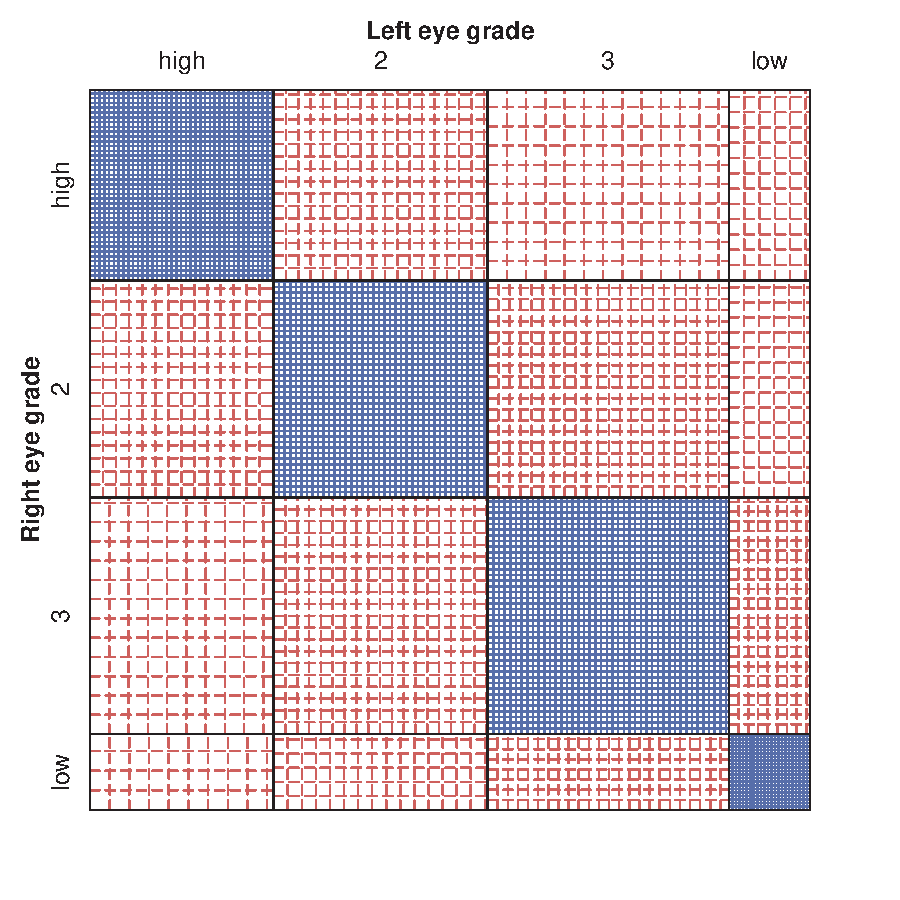
\includegraphics[width=.7\textwidth]{ch04/fig/VA-sieve2-1} }

\caption[Vision classification for 7477 women in Royal Ordnance factories]{Vision classification for 7477 women in Royal Ordnance factories. The high frequencies in the diagonal cells indicate the main association, but a subtler pattern also appears in the symmetric off-diagonal cells.\label{fig:VA-sieve2}}
\end{figure}


\end{knitrout}

The diagonal cells show the obvious:
people tend to have the same visual acuity in both eyes, and there is
strong lack of independence.  The off diagonal cells show a more subtle
pattern that suggests symmetry---the cells below the diagonal
are approximately equally dense as the corresponding cells above the diagonal.
Moreover, the relatively consistent pattern on the diagonals
$\pm 1, \pm 2, \dots$ away from the main diagonals suggests
that the association may be explained in terms of the \emph{difference}
in visual acuity between the two eyes.

These suggestions can be tested by fitting  intermediate models
between the null model of independence (which fits terribly)
and the saturated model (which fits perfectly),
as we shall see later in this book.
A model of \term{quasi-independence}, for example
(see \exref{ex:vision-glm} in \chref{ch:loglin})
ignores the diagonal cells and tests whether independence holds
for the remainder of the table.
The \term{symmetry} model for a square table allows association,
but constrains the expected frequencies above and below the
main diagonal to be equal.
Such models provide a
way of testing \emph{specific} explanatory models that relate to
substantive hypotheses and what we observe in our visualizations.
These and other models for square tables
are discussed further in \secref{sec:loglin-square}.
%\TODO{Add forward references to section(s) on models for square tables.}
\ixd{visual acuity}
\end{Example}

\subsection{Larger tables: The strucplot framework}\label{sec:twoway-sieve-larger}
The implementation of sieve diagrams in \pkg{vcd} is far more
general than illustrated in the examples above.  For one thing,
the \code{sieve} function has a formula method, which allows one to specify
the variables in the display as a model formula.
For example, for the \data{VisualAcuity} data, a plot of
the (marginal) frequencies for left and right eye grades
pooling over gender can be obtained with the call below
(this plot is not shown).

\begin{knitrout}
\definecolor{shadecolor}{rgb}{1, 0.961, 0.933}\color{fgcolor}\begin{kframe}
\begin{alltt}
\hlstd{> }\hlkwd{sieve}\hlstd{(Freq} \hlopt{~} \hlstd{right} \hlopt{+} \hlstd{left,}  \hlkwc{data} \hlstd{= VisualAcuity,} \hlkwc{shade} \hlstd{=} \hlnum{TRUE}\hlstd{)}
\end{alltt}
\end{kframe}
\end{knitrout}

More importantly, sieve diagrams are just one example of
the \term{strucplot framework}, a general system for
visualizing $n$-way frequency tables in a hierarchical
way.  We describe this framework in more detail in
\secref{sec:mosaic-strucplot} in context of mosaic
displays.  For now, we just illustrate the extension of
the formula method to provide for conditioning variables.
In the call below, the formula \verb#Freq ~ right + left | gender#
means to produce a separate block in the plot for the levels of
\var{gender}. The \code{set\_varnames} argument relabels the
variable names.
% \footnote{
% An equivalent plot, but one labeled more nicely, as in \figref{fig:VA-sieve2},
% can be produced from the \code{VA} table using
% \code{sieve(VA, shade = TRUE, condvar = "gender")}.
% }

\begin{knitrout}
\definecolor{shadecolor}{rgb}{1, 0.961, 0.933}\color{fgcolor}\begin{kframe}
\begin{alltt}
\hlstd{> }\hlkwd{sieve}\hlstd{(Freq} \hlopt{~} \hlstd{right} \hlopt{+} \hlstd{left} \hlopt{|} \hlstd{gender,}  \hlkwc{data} \hlstd{= VisualAcuity,} \hlkwc{shade} \hlstd{=} \hlnum{TRUE}\hlstd{,}
\hlstd{+ }      \hlkwc{set_varnames} \hlstd{=} \hlkwd{c}\hlstd{(}\hlkwc{right} \hlstd{=} \hlstr{"Right eye grade"}\hlstd{,} \hlkwc{left} \hlstd{=} \hlstr{"Left eye grade"}\hlstd{))}
\end{alltt}
\end{kframe}\begin{figure}[!htbp]

\centerline{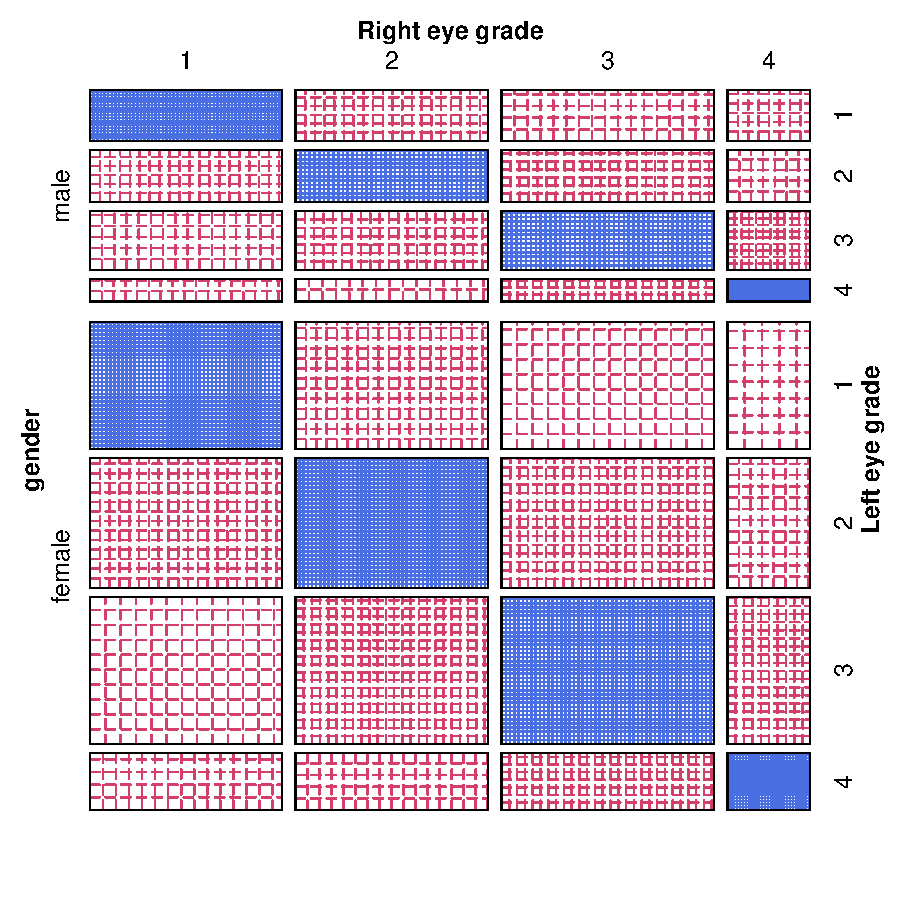
\includegraphics[width=.7\textwidth]{ch04/fig/VA-sieve3-1} }

\caption[Sieve diagram for the three-way table of VisualAcuity, conditioned on gender]{Sieve diagram for the three-way table of VisualAcuity, conditioned on gender.\label{fig:VA-sieve3}}
\end{figure}


\end{knitrout}

In \figref{fig:VA-sieve3}, the relative sizes of the blocks for the conditioning
variable (\var{gender}) show the much larger number of women than men in
this data.  Within each block, color and density of the box rules shows the
association of left and right acuity, and it appears that the pattern
for men is similar to that observed for women.

An alternative way of visualizing stratified data is a \term{coplot}
or \term{conditioning plot}, which, for each stratum, shows an
appropriate display for a subset of the data. Figure
\figref{fig:VA-cotabsieve3} visualizes separate sieve plots for men
and women:
\begin{knitrout}
\definecolor{shadecolor}{rgb}{1, 0.961, 0.933}\color{fgcolor}\begin{kframe}
\begin{alltt}
\hlstd{> }\hlkwd{cotabplot}\hlstd{(VA,} \hlkwc{cond} \hlstd{=} \hlstr{"gender"}\hlstd{,} \hlkwc{panel} \hlstd{= cotab_sieve,} \hlkwc{shade} \hlstd{=} \hlnum{TRUE}\hlstd{)}
\end{alltt}
\end{kframe}\begin{figure}[!htbp]

\centerline{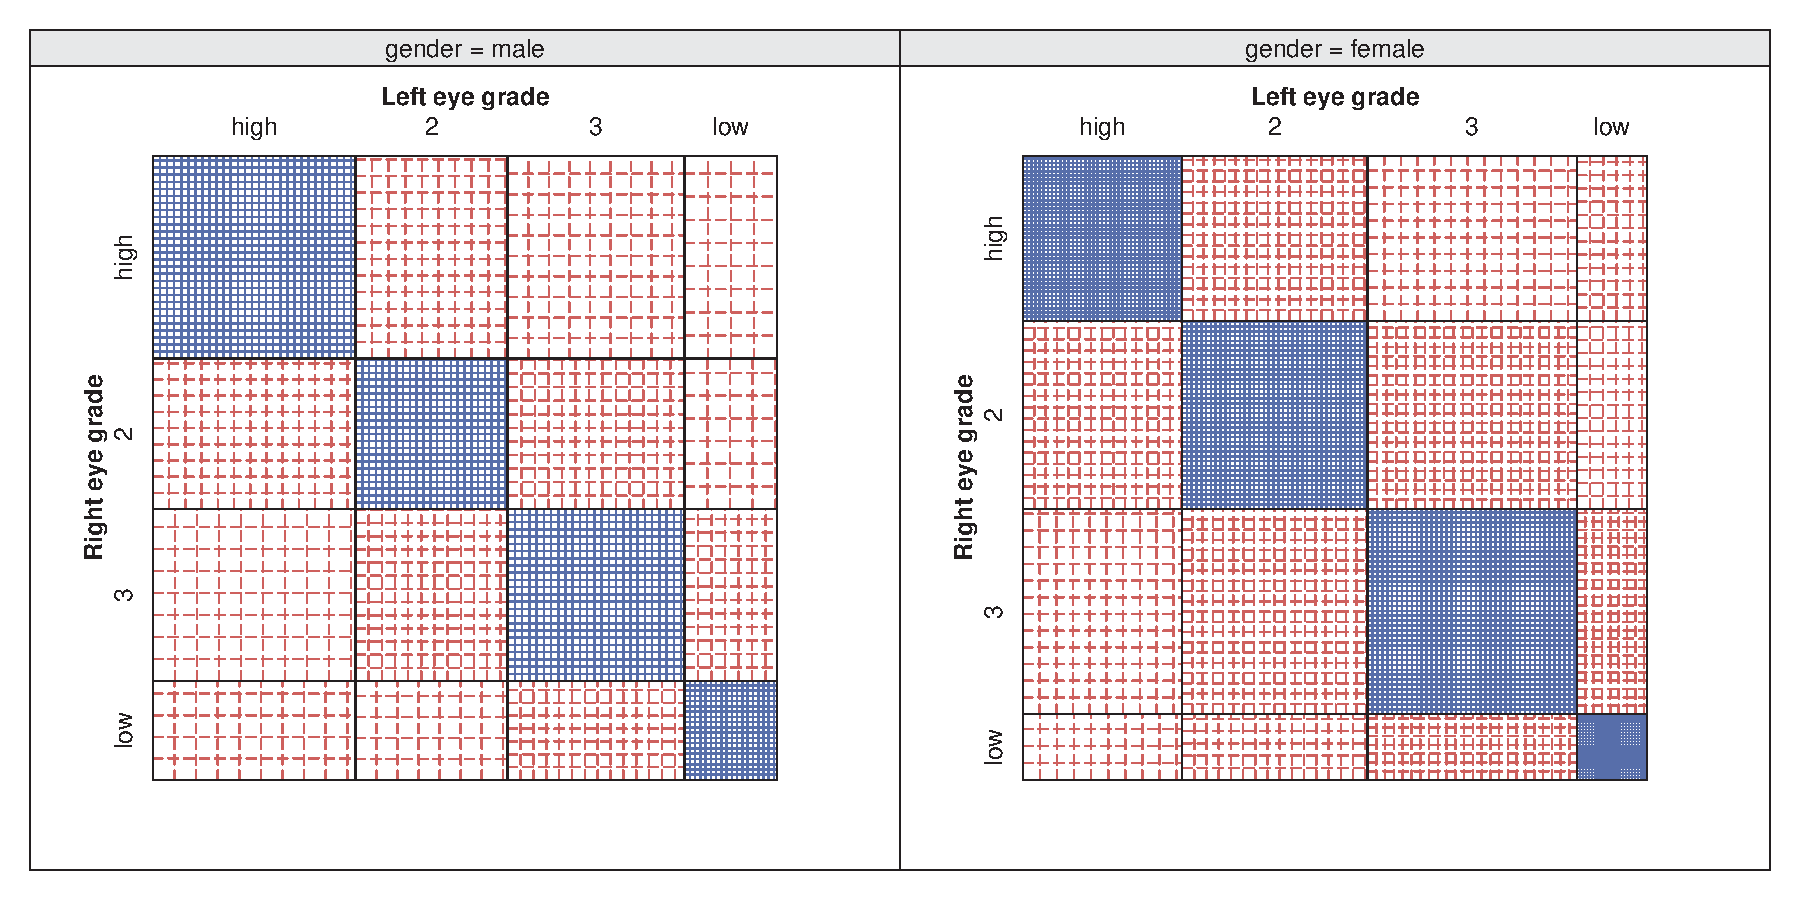
\includegraphics[width=\textwidth]{ch04/fig/VA-cotabsieve3-1} }

\caption[Conditional Sieve diagram for the three-way table of VisualAcuity, conditioned on gender]{Conditional Sieve diagram for the three-way table of VisualAcuity, conditioned on gender.\label{fig:VA-cotabsieve3}}
\end{figure}


\end{knitrout}
\noindent The main difference to the extended sieve plots is that the
distribution of the conditioning variable is not shown, which
basically is a lost of information, but advantageous if the distribution of the conditioning variable(s) is
highly skewed, since the partial displays of small strata will not be distorted.

The methods described in \secref{sec:twoway-homog} can be used to test
the hypothesis of homogeneity of association, and
\loglin models described in \chref{ch:loglin} provide
specific tests of hypotheses of \term{symmetry},
\term{quasi-independence} and other models for structured associations.

\begin{Example}[berkeley3]{Berkeley admissions}
This example illustrates some additional flexibility of sieve plots
with the strucplot framework, using the Berkeley admissions data.
The left panel of \figref{fig:berkeley-sieve} shows the sieve diagrams for
the relation between department and admission, conditioned by gender.
It can easily be seen that
\begin{seriate}
  \item overall, there were more male applicants than female;
  \item there is a moderately similar pattern of observed $>$ expected (blue)
  for males and females.
\end{seriate}
\begin{knitrout}
\definecolor{shadecolor}{rgb}{1, 0.961, 0.933}\color{fgcolor}\begin{kframe}
\begin{alltt}
\hlstd{> }\hlcom{# conditioned on gender}
\hlstd{> }\hlkwd{sieve}\hlstd{(UCBAdmissions,} \hlkwc{shade}\hlstd{=}\hlnum{TRUE}\hlstd{,} \hlkwc{condvar}\hlstd{=}\hlstr{'Gender'}\hlstd{)}
\hlstd{> }\hlcom{# three-way table, Department first, with cell labels}
\hlstd{> }\hlkwd{sieve}\hlstd{(}\hlopt{~} \hlstd{Dept} \hlopt{+} \hlstd{Admit} \hlopt{+} \hlstd{Gender,} \hlkwc{data} \hlstd{= UCBAdmissions,}
\hlstd{+ }      \hlkwc{shade} \hlstd{=} \hlnum{TRUE}\hlstd{,} \hlkwc{labeling} \hlstd{= labeling_values,}
\hlstd{+ }      \hlkwc{gp_text} \hlstd{=} \hlkwd{gpar}\hlstd{(}\hlkwc{fontface} \hlstd{=} \hlnum{2}\hlstd{),} \hlkwc{abbreviate_labs} \hlstd{=} \hlkwd{c}\hlstd{(}\hlkwc{Gender} \hlstd{=} \hlnum{TRUE}\hlstd{))}
\end{alltt}
\end{kframe}\begin{figure}[!htbp]

\centerline{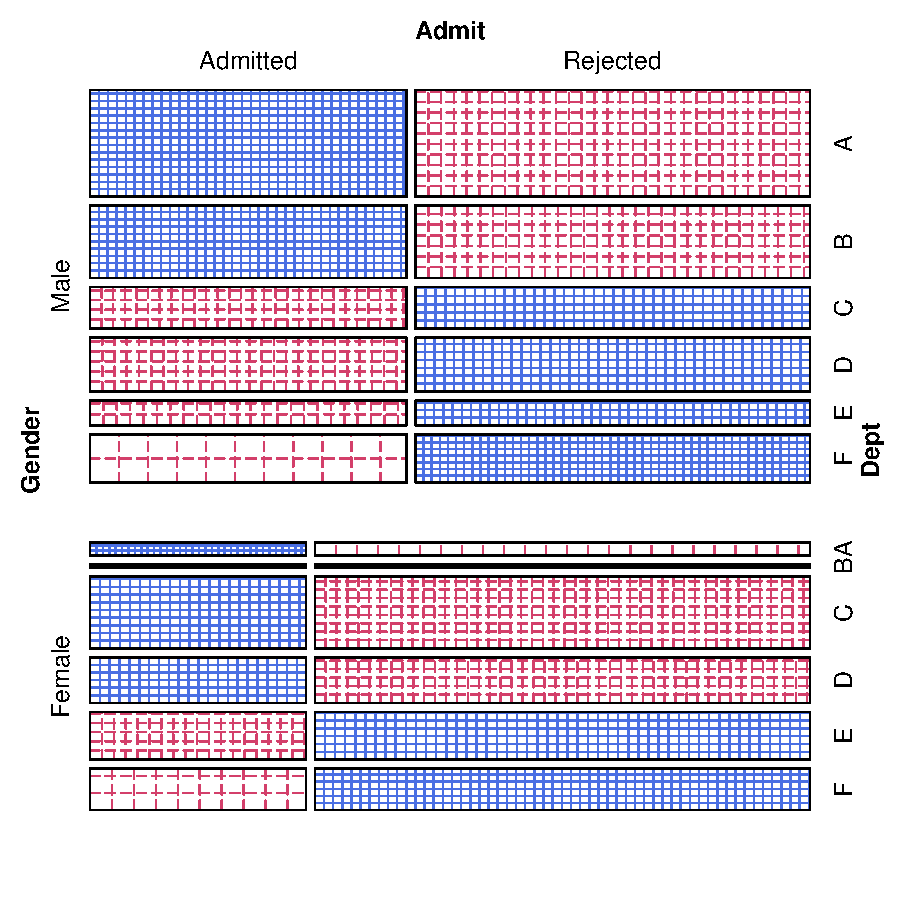
\includegraphics[width=.49\textwidth]{ch04/fig/berkeley-sieve-1} 
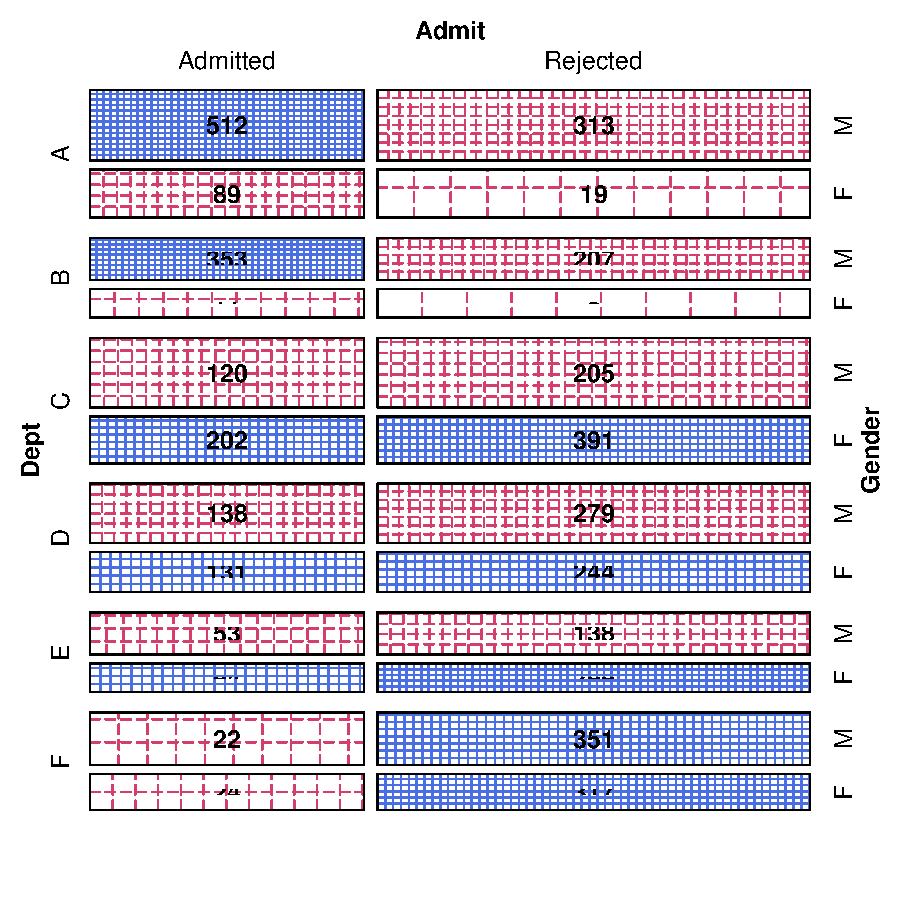
\includegraphics[width=.49\textwidth]{ch04/fig/berkeley-sieve-2} }

\caption[Sieve diagrams for the three-way table of the Berkeley admissions data]{Sieve diagrams for the three-way table of the Berkeley admissions data. Left: Admit by Dept, conditioned on Gender; right: Dept re-ordered as the first splitting variable.\label{fig:berkeley-sieve}}
\end{figure}


\end{knitrout}
In the right panel of \figref{fig:berkeley-sieve}, the three-way table
was first permuted to make \var{Dept} the first splitting variable.
Each $2 \times 2$ table of \var{Admit} by \var{Gender} then appears,
giving a sieve diagram version of what we showed earlier in
fourfold displays (\figref{fig:berk-fourfold4}).
The \code{labeling} argument is used here to write the cell frequency
in each rectangle. \code{gp_text} renders them in bold font, and
\code{abbreviate_labs} abbreviates the gender labels to avoid overplotting.

Alternatively, we can again use coplots to visualize conditioned sieve
plots for this data:

\begin{knitrout}
\definecolor{shadecolor}{rgb}{1, 0.961, 0.933}\color{fgcolor}\begin{kframe}
\begin{alltt}
\hlstd{> }\hlkwd{cotabplot}\hlstd{(UCBAdmissions,} \hlkwc{cond} \hlstd{=} \hlstr{"Gender"}\hlstd{,} \hlkwc{panel} \hlstd{= cotab_sieve,} \hlkwc{shade} \hlstd{=} \hlnum{TRUE}\hlstd{)}
\end{alltt}
\end{kframe}\begin{figure}[!htbp]

\centerline{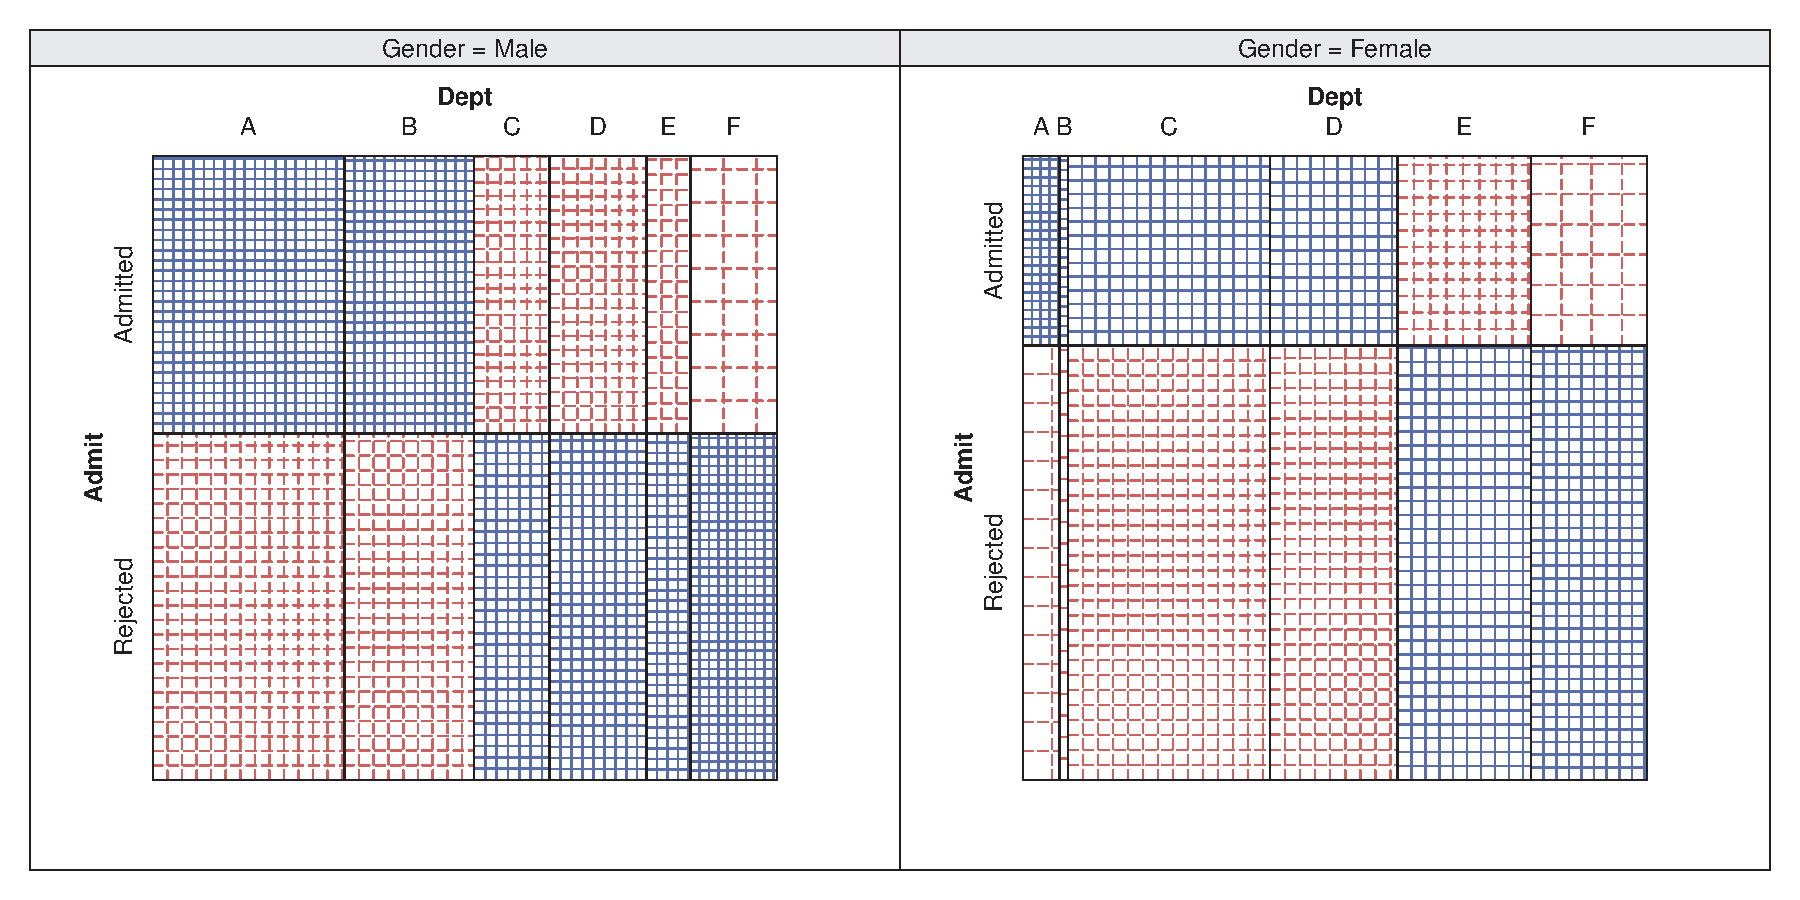
\includegraphics[width=\textwidth]{ch04/fig/berkeley-cotabsieve-1} }

\caption[Conditional Sieve diagram for the three-way table of the Berkeley data, conditioned on gender]{Conditional Sieve diagram for the three-way table of the Berkeley data, conditioned on gender.\label{fig:berkeley-cotabsieve}}
\end{figure}


\end{knitrout}
\begin{knitrout}
\definecolor{shadecolor}{rgb}{1, 0.961, 0.933}\color{fgcolor}\begin{kframe}
\begin{alltt}
\hlstd{> }\hlkwd{cotabplot}\hlstd{(UCBAdmissions,} \hlkwc{cond} \hlstd{=} \hlstr{"Dept"}\hlstd{,} \hlkwc{panel} \hlstd{= cotab_sieve,} \hlkwc{shade} \hlstd{=} \hlnum{TRUE}\hlstd{,}
\hlstd{+ }          \hlkwc{labeling} \hlstd{= labeling_values,} \hlkwc{gp_text} \hlstd{=} \hlkwd{gpar}\hlstd{(}\hlkwc{fontface} \hlstd{=} \hlstr{"bold"}\hlstd{))}
\end{alltt}
\end{kframe}\begin{figure}[!htbp]

\centerline{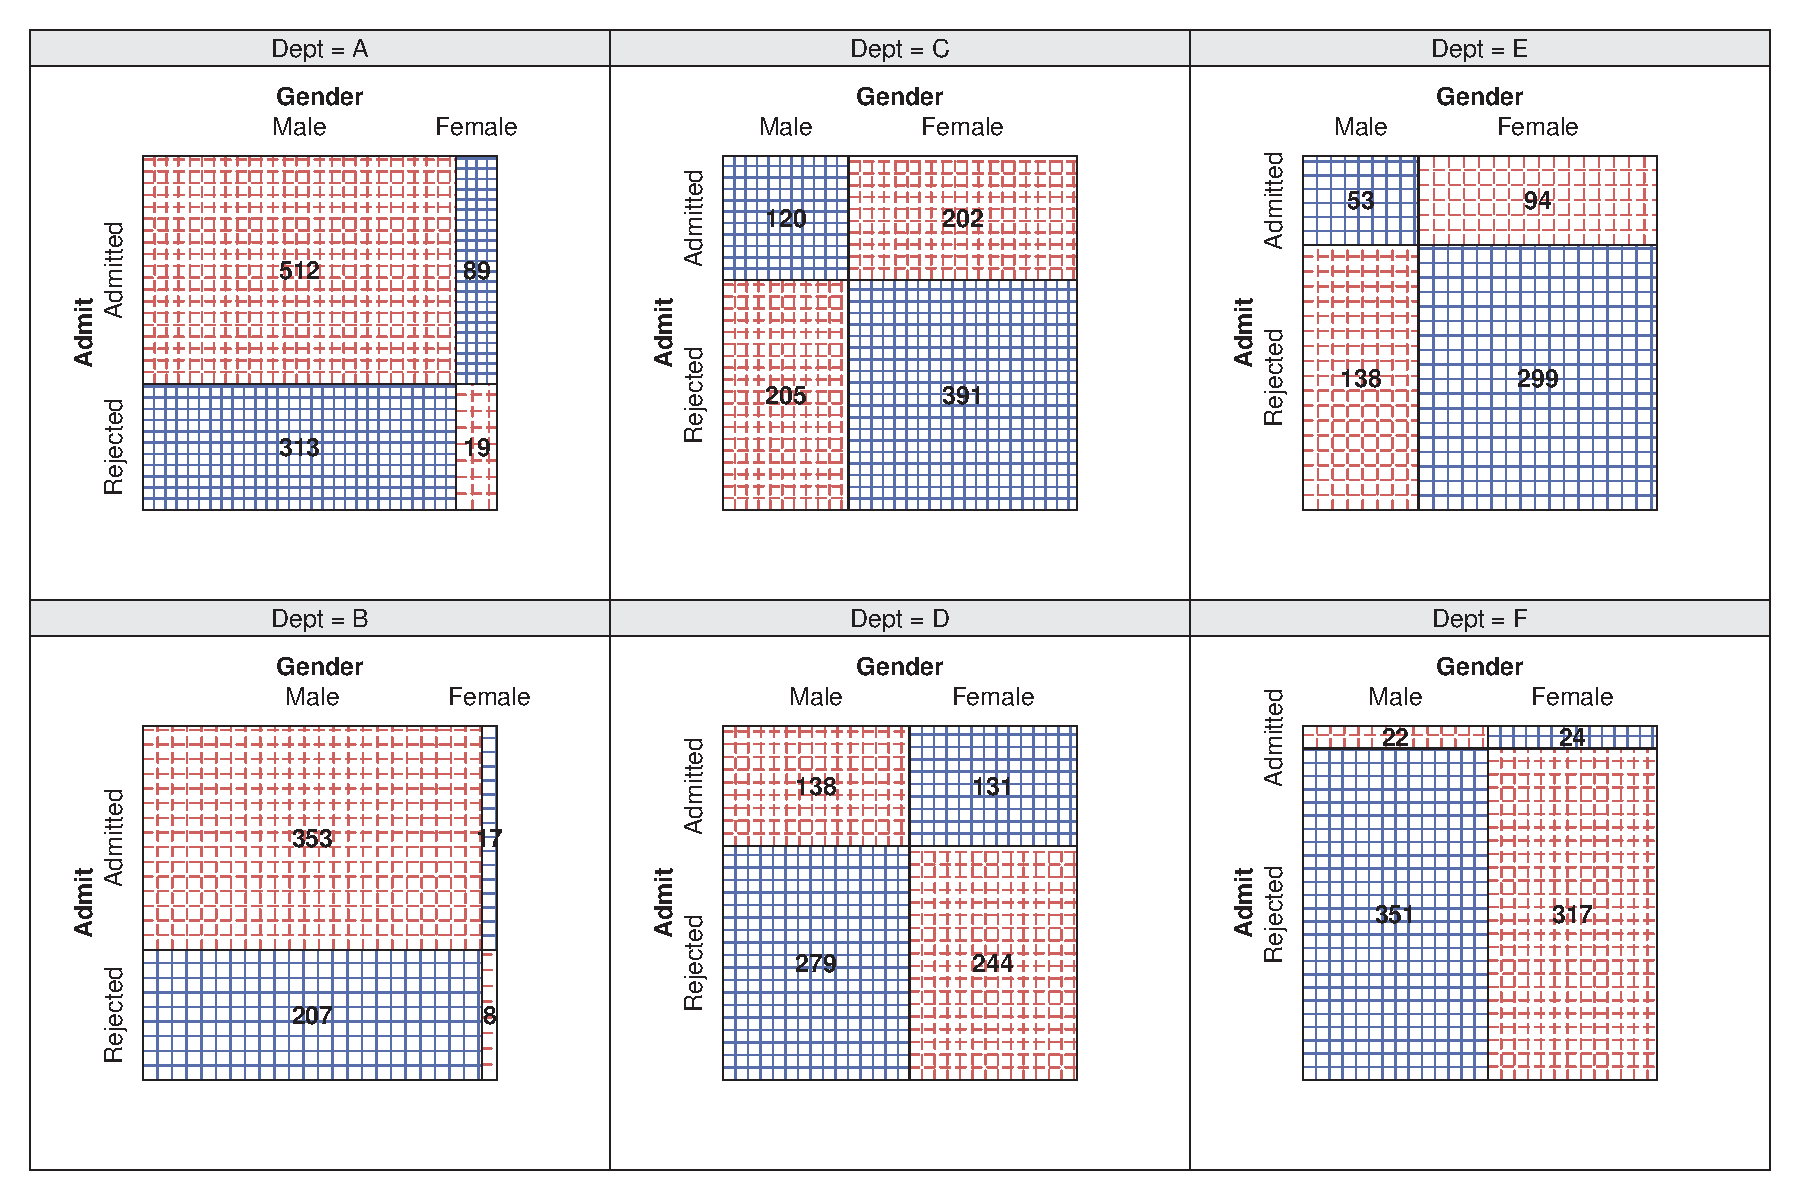
\includegraphics[width=\textwidth]{ch04/fig/berkeley-cotabsieve2-1} }

\caption[Conditional Sieve diagram for the three-way table of the Berkeley data, conditioned on department]{Conditional Sieve diagram for the three-way table of the Berkeley data, conditioned on department.\label{fig:berkeley-cotabsieve2}}
\end{figure}


\end{knitrout}

\subsubsection*{Remark}

Finally, for tables of more than two dimensions, there is a variety of
different models for ``independence'' (discussed in Chapter \ref{ch:loglin}
on log-linear models), and the strucplot framework
allows these to be specified with the \code{expected} argument,
either as an array of numbers conforming to the \code{data}
argument, or as a model formula for \func{loglm}.

For example, a sieve diagram may be used to determine if the association
between gender and department is the same across departments
by fitting the model \verb|~ Admit * Gender + Dept|, which
says that \var{Dept} is independent of the combinations of \code{Admit}
and \code{Gender}.  This is done as shown below, giving the plot in
\figref{fig:berkeley-sieve2}.

\begin{knitrout}
\definecolor{shadecolor}{rgb}{1, 0.961, 0.933}\color{fgcolor}\begin{kframe}
\begin{alltt}
\hlstd{> }\hlstd{UCB2} \hlkwb{<-} \hlkwd{aperm}\hlstd{(UCBAdmissions,} \hlkwd{c}\hlstd{(}\hlnum{3}\hlstd{,} \hlnum{2}\hlstd{,}\hlnum{1}\hlstd{))}
\hlstd{> }\hlkwd{sieve}\hlstd{(UCB2,} \hlkwc{shade} \hlstd{=} \hlnum{TRUE}\hlstd{,} \hlkwc{expected} \hlstd{=} \hlopt{~} \hlstd{Admit} \hlopt{*} \hlstd{Gender} \hlopt{+} \hlstd{Dept,}
\hlstd{+ }      \hlkwc{split_vertical} \hlstd{=} \hlkwd{c}\hlstd{(}\hlnum{FALSE}\hlstd{,} \hlnum{TRUE}\hlstd{,} \hlnum{TRUE}\hlstd{))}
\end{alltt}
\end{kframe}\begin{figure}[!htbp]

\centerline{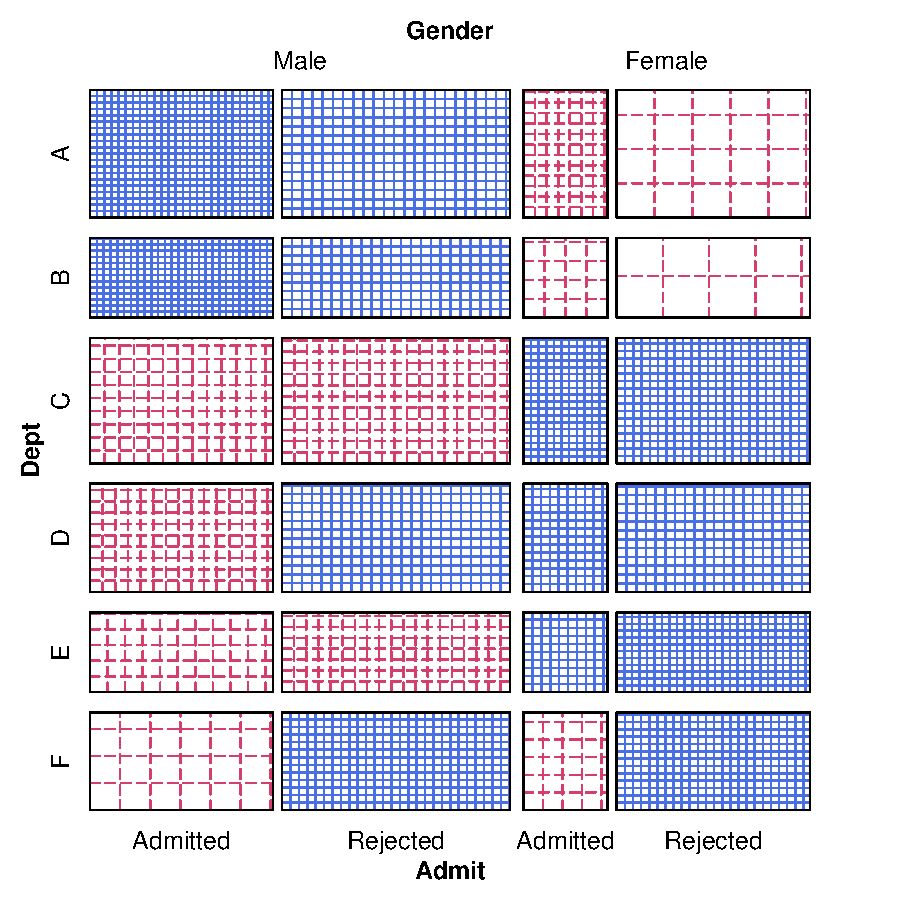
\includegraphics[width=.6\textwidth]{ch04/fig/berkeley-sieve2-1} }

\caption[Sieve diagram for the Berkeley admissions data, fitting the model of joint independence, Admit *Gender + Dept]{Sieve diagram for the Berkeley admissions data, fitting the model of joint independence, Admit *Gender + Dept\label{fig:berkeley-sieve2}}
\end{figure}


\end{knitrout}
In terms of the \loglin models discussed in
\chref{ch:mosaic}, this is equivalent to fitting the model
of \term{joint independence}, $\llmtwo{AdmitGender}{Dept}$.
\figref{fig:berkeley-sieve2} shows the greater numbers of
male applicants in departments A and B
(whose overall rate of admission is high) and greater numbers of female
applicants in the remaining departments (where the admission rate is low).

\end{Example}
\ixoff{sieve diagram}

\section{Association plots}\label{sec:twoway-assoc}
In the \IX{sieve diagram} the foreground (rectangles) shows expected
frequencies; deviations from independence are shown by color and
density of shading.  The \term{association plot}
\citep{Cohen:80,Friendly:91}
puts deviations from independence in the foreground:  the area
of each box is made proportional to the
(observed $-$ expected) frequency.
%This graphical method is described in more detail in \SSSGref{10.2.1},
%which also lists the program used to produce the association plot.

For a two-way contingency table, the signed contribution to Pearson
\(\chi^2\) for cell \(i, \, j\) is
\begin{equation}\label{eq:Pearson-residual}
  d_{ij}  =
  \frac{ n_{ij} - m_{ij} } { \sqrt { m_{ij} } }
 = \mbox{ Pearson residual},
  \qquad
  \chi^2 = \sum_{ij} \:  ( d_{ij} )^2
\end{equation}

In the association plot, each cell is shown by a
rectangle, having:

\begin{itemize*}
\item (signed) height \(\sim d_{ij}\)

\item width = \(\sqrt { m_{ij}}\).
\end{itemize*}
so, the area of each cell is proportional to the raw residual,
%\glosstex{residuals}
\(n_{ij} - m_{ij}\).
The rectangles for each row in the table are positioned relative to a
baseline representing independence (\(d_{ij} = 0\)) shown by a dotted
line.  Cells with observed \(>\) expected frequency rise above the line
(and are colored blue); cells that contain less than the expected
frequency fall below it (and are shaded red).
\begin{knitrout}
\definecolor{shadecolor}{rgb}{1, 0.961, 0.933}\color{fgcolor}\begin{kframe}
\begin{alltt}
\hlstd{> }\hlkwd{assoc}\hlstd{(}\hlopt{~} \hlstd{Hair} \hlopt{+} \hlstd{Eye,} \hlkwc{data} \hlstd{= HairEyeColor,} \hlkwc{shade} \hlstd{=} \hlnum{TRUE}\hlstd{)}
\hlstd{> }\hlkwd{assoc}\hlstd{(HairEyeColor,} \hlkwc{shade} \hlstd{=} \hlnum{TRUE}\hlstd{)}
\end{alltt}
\end{kframe}
\end{knitrout}
\begin{knitrout}
\definecolor{shadecolor}{rgb}{1, 0.961, 0.933}\color{fgcolor}\begin{figure}[!htbp]

\centerline{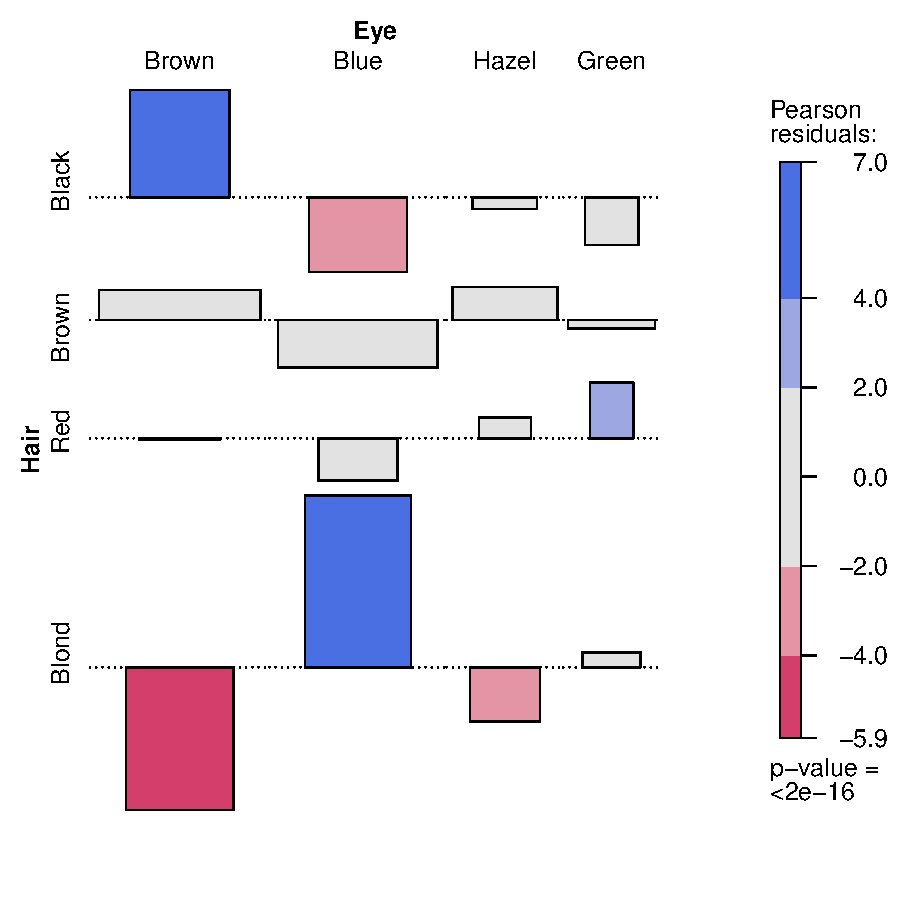
\includegraphics[width=0.5\textwidth]{ch04/fig/HE-assoc-1} 
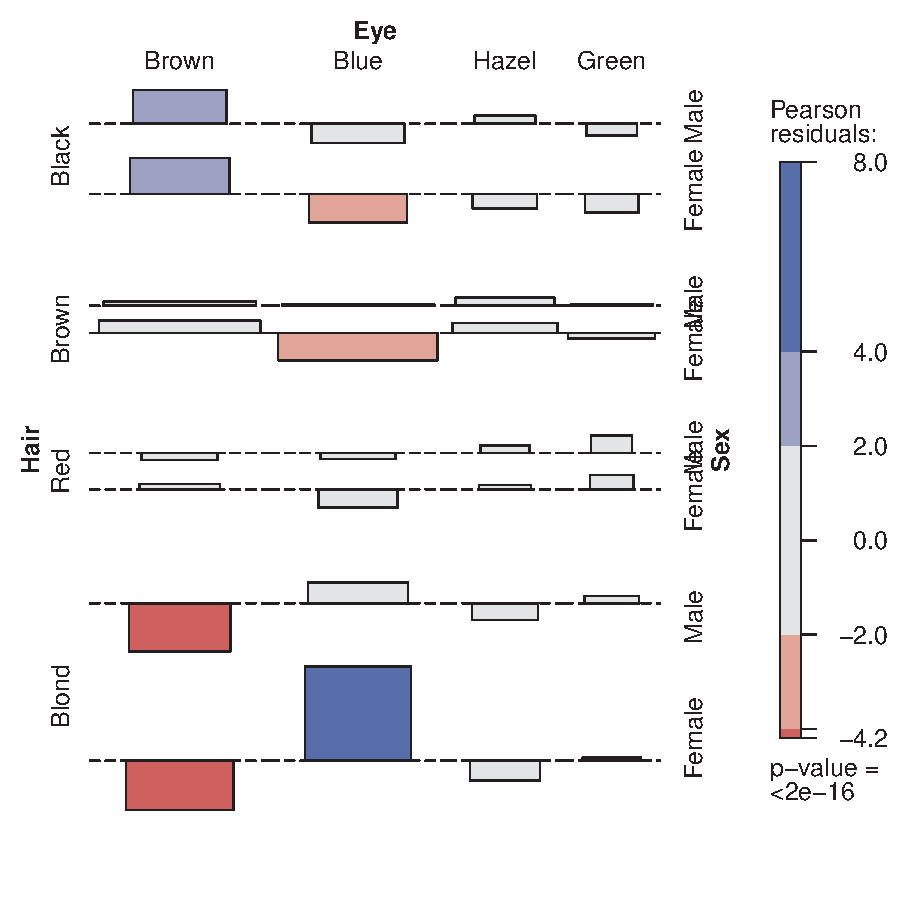
\includegraphics[width=0.5\textwidth]{ch04/fig/HE-assoc-2} }

\caption[Association plot for the hair-color eye-color data]{Association plot for the hair-color eye-color data. Left: marginal table, collapsed over gender; right: full table.\label{fig:HE-assoc}}
\end{figure}


\end{knitrout}
\figref{fig:HE-assoc} (left) shows the association plot for the data on
hair color and eye color.
In constructing this plot, each rectangle is shaded according to
the value of the Pearson residual \eqref{eq:Pearson-residual},
using a simple scale shown in the legend, where residuals
$|d_{ij}| > 2$ are shaded blue or red depending on their sign
and residuals $|d_{ij}| > 4$
are shaded with a more saturated color.

One virtue of the association plot is that it is quite simple to
interpret in terms of the pattern of
positive and negative  $d_{ij}$ values.
\citet{Bertin:81} uses similar graphics to display large complex
\ctabs.  Like the sieve diagram, however, patterns of association
are most apparent when the rows and columns of the display are ordered
in a sensible way.

We note here that the association plot also belongs to the
strucplot framework and thus extends to higher-way tables.
For example, the full \data{HairEyeColor} table is
also classified by \var{Sex}.
The plot for the three-way table
is shown in \figref{fig:HE-assoc} (right).
%\TODO{Perhaps combine these two figures into two panels, side by side.}
In this plot the third table
variable (\var{Sex} here) is shown nested within the first two,
allowing easy comparison of the profiles of hair and eye color
for males and females.


\section{Observer agreement}\label{sec:twoway-agree}

When the row and column variables represent different
observers rating the same subjects or objects, interest is focused on
\term{observer agreement} rather than mere association.
In this case, measures and tests
of agreement provide a method of assessing the
reliability of a subjective classification or assessment procedure.

For example, two (or more) clinical psychologists might classify
patients on a scale with categories
\begin{seriate}
\item normal,
\item mildly impaired,
\item severely impaired.
\end{seriate}
Or, ethologists might classify the behavior
of animals in categories of cooperation, dominance and so forth,
or paleologists might classify pottery fragments according to
categories of antiquity or cultural groups. As these examples
suggest, the rating categories are often ordered, but not always.

For two raters, a
contingency table can be
formed classifying all the subjects/objects rated
according to the rating categories used by the two
observers.
In most cases, the same categories are used by both raters,
so the \ctab is square, and the entries in the diagonal cells
are the cases where the raters agree.

In this section we describe some measures of the strength
of agreement and then a method for visualizing the pattern of
agreement.  But first, the following examples show some
typical agreement data.

\begin{Example}[sexisfun1]{Sex is fun}
The \data{SexualFun} table in \pkg{vcd}
%\tabref{tab:sexisfun}
(\citet[Table 2.10]{Agresti:90}, from \citet{Hout-etal:87})
 summarizes the responses of 91
married couples to a questionnaire item:
%\begin{quote}
``Sex is fun for me and my partner:
\begin{seriate}
  \item Never or occasionally,
  \item fairly often,
  \item very often,
  \item almost always.
\end{seriate}
%\end{quote}
''
\begin{knitrout}
\definecolor{shadecolor}{rgb}{1, 0.961, 0.933}\color{fgcolor}\begin{kframe}
\begin{alltt}
\hlstd{> }\hlkwd{data}\hlstd{(}\hlstr{"SexualFun"}\hlstd{,} \hlkwc{package} \hlstd{=} \hlstr{"vcd"}\hlstd{)}
\hlstd{> }\hlstd{SexualFun}
\end{alltt}
\begin{verbatim}
              Wife
Husband        Never Fun Fairly Often Very Often Always fun
  Never Fun            7            7          2          3
  Fairly Often         2            8          3          7
  Very Often           1            5          4          9
  Always fun           2            8          9         14
\end{verbatim}
\end{kframe}
\end{knitrout}

In each row the diagonal entry is not always the largest, though it
appears that the partners tend to agree more often when either responds
``almost always''.
%\begin{table}[htb]
\caption[Ratings of a questionnaire item, ``Sex is fun'', by husbands and wives]{Ratings of a questionnaire item, ``Sex is fun'', by husbands and wives. Source: \citet[Table 2.10]{Agresti:90}, from Hout \etal.}\label{tab:sexisfun}
\begin{center}
 \begin{tabular}{l|rrrr|r}
  \hline
            & \multicolumn{4}{c|}{Wife's Rating} & \\
  Husband's & Never & Fairly & Very & Almost &  \\ 
  Rating & fun & often & Often & always & Total \\ 
  \hline
  Never fun     & 7 & 7 & 2 & 3 & 19 \\ 
  Fairly often  & 2 & 8 & 3 & 7 & 20 \\ 
  Very often    & 1 & 5 & 4 & 9 & 19 \\ 
  Almost always & 2 & 8 & 9 & 14 & 33 \\ 
  \hline
  Total & 12 & 28 & 18 & 33 & 91 \\ 
  \hline
 \end{tabular}
\end{center}
\end{table}

\end{Example}

\begin{Example}[MS1]{Diagnosis of MS patients}
\citet{LandisKoch:77} gave data on the diagnostic classification
of multiple sclerosis (MS) patients by two neurologists,
one from Winnipeg and one from New Orleans.
There were two samples of patients, 149 from Winnipeg and
69 from New Orleans, and each neurologist classified
all patients
into one of four diagnostic categories:
\begin{seriate}
\item Certain MS,
\item Probable MS,
\item Possible MS,
\item Doubtful, unlikely, or definitely not MS
\end{seriate}

These data are available in \data{MSPatients},
a $4 \times 4 \times 2$ table, as shown below.
It is convenient to show the data in separate slices for the Winnipeg
and New Orleans patients:
\begin{knitrout}
\definecolor{shadecolor}{rgb}{1, 0.961, 0.933}\color{fgcolor}\begin{kframe}
\begin{alltt}
\hlstd{> }\hlstd{MSPatients[, ,} \hlstr{"Winnipeg"}\hlstd{]}
\end{alltt}
\begin{verbatim}
                       Winnipeg Neurologist
New Orleans Neurologist Certain Probable Possible Doubtful
               Certain       38        5        0        1
               Probable      33       11        3        0
               Possible      10       14        5        6
               Doubtful       3        7        3       10
\end{verbatim}
\begin{alltt}
\hlstd{> }\hlstd{MSPatients[, ,} \hlstr{"New Orleans"}\hlstd{]}
\end{alltt}
\begin{verbatim}
                       Winnipeg Neurologist
New Orleans Neurologist Certain Probable Possible Doubtful
               Certain        5        3        0        0
               Probable       3       11        4        0
               Possible       2       13        3        4
               Doubtful       1        2        4       14
\end{verbatim}
\begin{alltt}
\hlstd{> }\hlkwd{apply}\hlstd{(MSPatients,} \hlnum{3}\hlstd{, sum)}      \hlcom{# show sample sizes}
\end{alltt}
\begin{verbatim}
   Winnipeg New Orleans 
        149          69 
\end{verbatim}
\end{kframe}
\end{knitrout}
In this example, note that the distribution of degree of severity of
MS may differ between the two patient samples.  As well, for a
given sample, the two neurologists may be more or less strict about
the boundaries between the rating categories.

%The data from the 69 patients in the New Orleans sample are shown in
%\tabref{tab:msdiag}.
%There appears to be highest agreement in the Doubtful category, followed by
%the Probable category.
%\begin{table}[htb]
\caption{Ratings of 69 patients by two neurologists}\label{tab:msdiag}
\begin{center}
 \begin{tabular}{l|rrrr|r}
  \hline
  New Orleans & \multicolumn{4}{c|}{Winnipeg Neurologist} & \\
  Neurologist & Certain & Probable & Possible & Doubtful & Total \\ 
  \hline
  Certain  MS & 5 & 3 & 0 & 0 & 8 \\ 
  Probable MS & 3 & 11 & 4 & 0 & 18 \\ 
  Possible MS & 2 & 13 & 3 & 4 & 22 \\ 
  Doubtful MS & 1 & 2 & 4 & 14 & 21 \\ 
  \hline
  Total       & 11 & 29 & 11 & 18 & 69 \\ 
  \hline
 \end{tabular}
\end{center}
\end{table}


\end{Example}

\subsection{Measuring agreement}\label{sec:agreemeas}
In assessing the strength of \emph{agreement} we usually have a more
stringent criterion than in measuring the strength of \emph{association},
because observers ratings can be strongly associated without strong agreement.
For example, one rater could use a more stringent criterion and thus consistently rate subjects one category lower (on an ordinal scale) then another rater.

More generally, measures of agreement must take account of the
marginal frequencies with which two raters use the categories.
If observers tend to use the categories
with different frequency, this will affect measures of
agreement.
\ix{marginal homogeneity}

Here we describe some simple indices that summarize agreement with a
single score (and associated standard errors or confidence intervals).
\citet{vonEyeMun:2006} treat this topic from the perspective of
\loglin models.

\subsubsection{Intraclass correlation}
\ix{intraclass correlation}
\ix{agreement!intraclass correlation}
An analysis of variance framework leads to the {\bf intraclass correlation}
as a measure of inter-rater reliability, particularly when there are
more than two raters.
This approach is not covered here, but various applications are described
by \citet{ShroutFleiss:79}, and implemented in \R in \func{ICC}
in the \Rpackage{psych}.

\subsubsection{Cohen's Kappa}
\ix{agreement!Cohen's $\kappa$}
\ix{Cohen's $\kappa$|(}

Cohen's kappa (\(\kappa\))
\citep{Cohen:60,Cohen:68} is a commonly used measure of agreement that
compares the observed agreement to agreement expected by chance if the two observer's
ratings were independent.
If $p_{ij}$ is the probability that a randomly selected subject is
rated in category $i$ by the first observer and in category $j$ by
the other, then the observed agreement is the sum of the diagonal
entries,  \(P_o  = \sum_i p_{ii}\).  If the ratings were independent,
this probability of agreement (by chance) would be \(P_c = \sum_i p_{i+} \,  p_{+i}\).
Cohen's $\kappa$ is then the ratio of the difference between actual
agreement and chance agreement, $P_o - P_c$, to the maximum value
this difference could obtain:

\begin{equation}\label{eq:kappa}
  \kappa =  \frac{ P_o - P_c } { 1 - P_c }
  \period
\end{equation}

When agreement is perfect, \(\kappa = 1\);  when agreement is no
better than would be obtained from statistically independent ratings,
$\kappa = 0$.
$\kappa$ could conceivably be negative, but this rarely occurs in practice.
The minimum possible value depends on the marginal totals.

For large samples ($n_{++}$), $\kappa$ has an approximate normal
distribution when $H_0 : \kappa = 0$ is true
and its standard error \citep{Fleiss:73,Fleiss-etal:69} is given by
\begin{equation*}
 \hat{\sigma}(\kappa) =  \frac{ P_c + P_c^2 - \sum_i p_{i+} p_{+i} (p_{i+} + p_{+i}) } { n_{++} (1 - P_c)^2 }
 \period
\end{equation*}
Hence, it is common to conduct a test of $H_0 : \kappa = 0$ by
referring $z = \kappa / \hat{\sigma}(\kappa)$
to a unit normal distribution.
The hypothesis of agreement no better than chance is rarely of much
interest, however.  It is preferable to estimate and report a
confidence interval for $\kappa$.

\subsubsection{Weighted Kappa}
The original (unweighted) \(\kappa\) only counts strict agreement (the same
category is assigned by both observers).  A weighted version of
\(\kappa\)
\citep{Cohen:68} may be used when one wishes to allow for \emph{partial} agreement.
For example, exact agreements might be given full weight,
one-category difference given weight 1/2.  This typically makes sense
only when the categories are \emph{ordered}, as in severity of
diagnosis.

Weighted \(\kappa\) uses weights, $0 \le w_{ij} \le 1$ for each cell in the
table, with $w_{ii} =1$ for the diagonal cells.
In this case $P_o$ and $P_c$ are defined as weighted sums
\begin{eqnarray*}
P_o  & = & \sum_i \sum_j w_{ij} p_{ij} \\
P_c  & = & \sum_i \sum_j w_{ij} p_{i+} p_{+j}\\
\end{eqnarray*}
and these weighted sums are used in \eqref{eq:kappa}.

For an $r \times r$ table, two commonly-used pattern of weights are those based on
equal spacing of weights
\citep{CicchettiAllison:71}
for a near-match,
%$w_{ij} = 1 - \frac{|i-j|}{r-1}$
and
\emph{Fleiss-Cohen weights}
\citep{FleissCohen:73}, based on an inverse-square
spacing,
% $w_{ij} = 1 - \frac{|i-j|^2}{(r-1)^2}$.
\begin{eqnarray*}
w_{ij} = & 1 - \frac{|i-j|}{r-1} & \quad\quad\mbox{equal spacing} \\
w_{ij} = & 1 - \frac{|i-j|^2}{(r-1)^2} & \quad\quad\mbox{Fleiss-Cohen}
\end{eqnarray*}
The Fleiss-Cohen weights attach greater importance
to near disagreements, as you can see below for a $4 \times 4$ table.
These weights also provide a measure equivalent to the intraclass
correlation.

\begin{verbatim}
       Integer Spacing                Inverse Square Spacing
   Cicchetti Allison weights           Fleiss-Cohen weights
 ----------------------------       ---------------------------
   1     2/3     1/3       0          1     8/9     5/9      0
 2/3       1     2/3     1/3        8/9       1     8/9    5/9
 1/3     2/3       1     2/3        5/9     8/9       1    8/9
   0     1/3     2/3       1          0     5/9     8/9      1
\end{verbatim}

\subsubsection{Computing Kappa}

The function \func{Kappa} in \pkg{vcd} calculates unweighted and weighted
Kappa.  The \code{weights} argument can be used to specify the weighting
scheme as either \code{"Equal-Spacing"} or \code{"Fleiss-Cohen"}.
The function returns a \class{Kappa} object, for which there
is a \func{confint.Kappa} method, providing confidence intervals.
The \func{summary.Kappa} method also prints the weights.

The lines below illustrate \code{Kappa} for the \data{SexualFun} data.
\begin{knitrout}
\definecolor{shadecolor}{rgb}{1, 0.961, 0.933}\color{fgcolor}\begin{kframe}
\begin{alltt}
\hlstd{> }\hlkwd{Kappa}\hlstd{(SexualFun)}
\end{alltt}
\begin{verbatim}
           value    ASE    z
Unweighted 0.129 0.0686 1.89
Weighted   0.237 0.0783 3.03
\end{verbatim}
\begin{alltt}
\hlstd{> }\hlkwd{confint}\hlstd{(}\hlkwd{Kappa}\hlstd{(SexualFun))}
\end{alltt}
\begin{verbatim}
            
Kappa               lwr     upr
  Unweighted -0.0051204 0.26378
  Weighted    0.0838834 0.39088
\end{verbatim}
\end{kframe}
\end{knitrout}

\TODO{DM: Add P-values?}
%\TODO{BUG: The result for weighted Kappa doesn't match that in Output 3.1 in vcd, and
%spoils the point about weighted kappa being more sensitive to near agreement.}
% Fixed by D.M.

\subsection[Observer Agreement Chart]{Observer Agreement Chart}
\label{sec:twoway-Bangdiwala}
\ixon{agreement!observer agreement chart}
\ixon{observer agreement chart}
The observer agreement chart proposed by Bangdiwala
\citeyearpar{Bangdiwala:1985,Bangdiwala:87} provides a simple
graphic representation of the strength of agreement in a contingency
table, and alternative measures of strength of agreement with an intuitive
interpretation. More importantly, it shows the \emph{pattern} of disagreement
when agreement is less than perfect.

\subsubsection{Construction of the basic plot}

Given a $k \times k$ contingency table, the agreement chart is constructed as an \(n \times  n\) square,
where $n = n_{++}$ is the total sample size.  Black squares, each of size
\(n_{ii} \times  n_{ii}\), show observed agreement.  These are positioned
within $k$ larger rectangles, each of size \(n_{i+} \times  n_{+i}\)
as shown in the left panel of
\figref{fig:sexfun-agree}.  
Each rectangle is subdivided by the row/column frequencies $n_{ij}$ of
row $i$/column $j$, where cell $(i, i)$ is filled black. The
large rectangle shows the maximum possible agreement, given the
marginal totals.  Thus, a visual impression of the strength of
agreement is given by
\begin{equation}\label{eq:bangb}
  B  =
  \frac{ \mbox{area of dark squares}}
  { \mbox{area of rectangles}}  =
  \frac{ \sum_i^k \,  n_{ii}^2 }
  { \sum_i^k \,  n_{i+} \,  n_{+i} }
\end{equation}
When there is perfect agreement, the $k$ rectangles determined by the
marginal totals are all squares, completely filled by the shaded squares
reflecting the diagonal $n_{ii}$ entries, and $B = 1$.
\begin{knitrout}
\definecolor{shadecolor}{rgb}{1, 0.961, 0.933}\color{fgcolor}\begin{kframe}
\begin{alltt}
\hlstd{> }\hlkwd{agreementplot}\hlstd{(SexualFun,} \hlkwc{main} \hlstd{=} \hlstr{"Unweighted"}\hlstd{,} \hlkwc{weights} \hlstd{=} \hlnum{1}\hlstd{)}
\hlstd{> }\hlkwd{agreementplot}\hlstd{(SexualFun,} \hlkwc{main} \hlstd{=} \hlstr{"Weighted"}\hlstd{)}
\end{alltt}
\end{kframe}\begin{figure}[!htbp]

\centerline{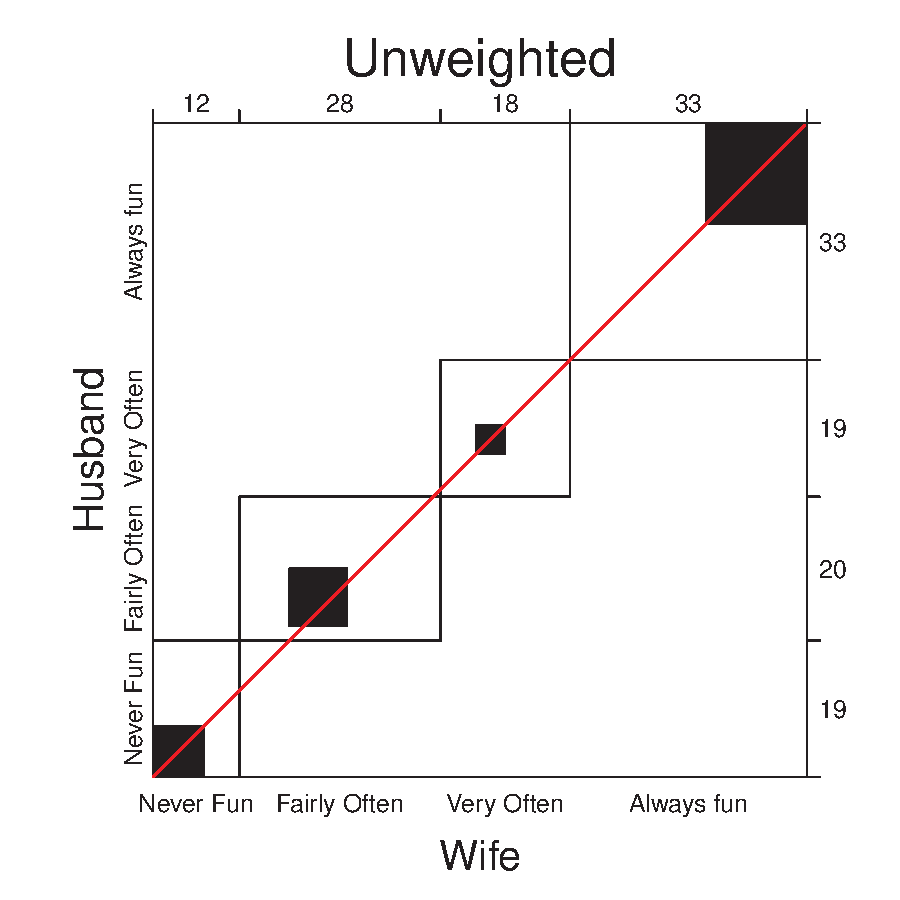
\includegraphics[width=.48\textwidth]{ch04/fig/sexfun-agree-1} 
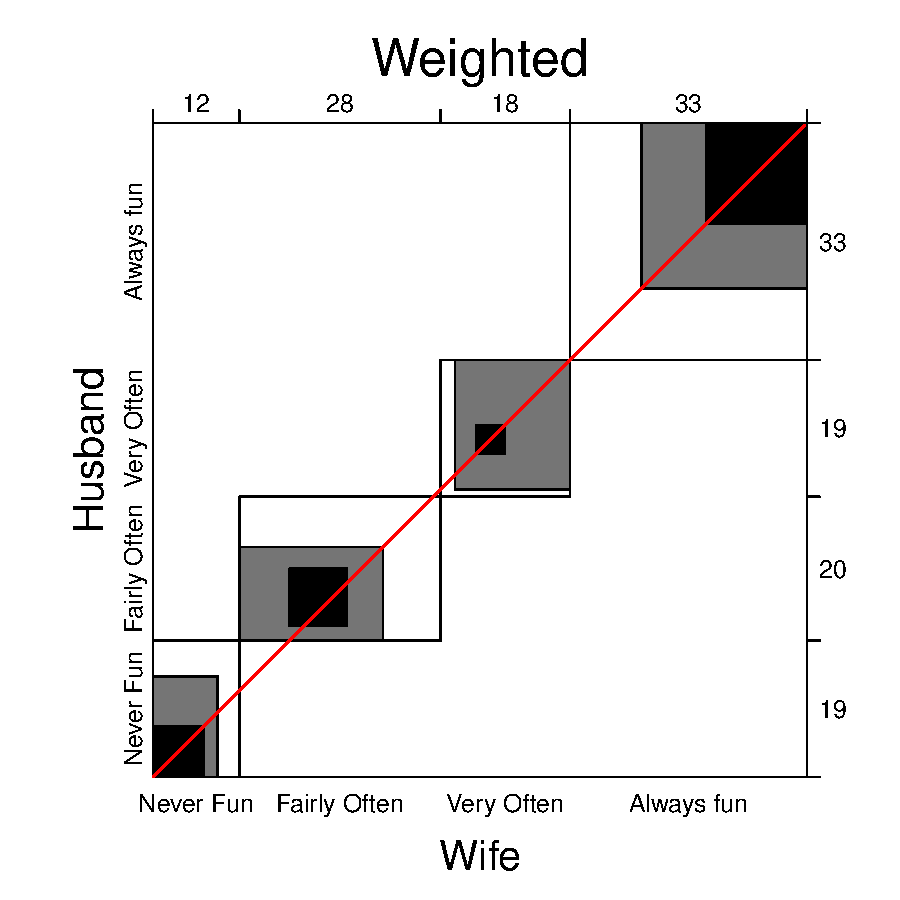
\includegraphics[width=.48\textwidth]{ch04/fig/sexfun-agree-2} }

\caption[Agreement charts for husbands' and wives' sexual fun]{Agreement charts for husbands' and wives' sexual fun. Left: unweighted chart, showing only exact agreement; right: weighted chart, using weight $w_1 = 8/9$ for a one-step disagreement.\label{fig:sexfun-agree}}
\end{figure}


\end{knitrout}
%\TODO{These figures are cut off on the margins for some reason. Correct this.}

\subsubsection{Partial agreement}
\ix{agreement!partial}
 Partial agreement is allowed by
including a weighted contribution from off-diagonal cells, $b$
steps from the main diagonal.  For a given cell frequency,
$n_{ij}$, a pattern of weights, $w_1, w_2, \dots,  w_b$ is applied
to the cell frequencies
as shown schematically below:
\begin{equation*}
 \left.
 \begin{array}{ccccc}
   &  & n_{i-b,i} &  & \\
        &  & \vdots    &  & \\
        n_{i, i-b} & \cdots & n_{i, i} & \cdots & n_{i, i+b} \\
        &  & \vdots    &  & \\
   &  & n_{i-b,i} &  &
 \end{array}
  \right.
  \qquad \Leftarrow \quad
 \left.
 \begin{array}{ccccc}
   &  & w_b &  & \\
   &  & \vdots &  & \\
 w_b & \cdots & 1 & \cdots & w_b \\
   &  & \vdots &  & \\
   &  & w_b &  & \\
 \end{array}
  \right.
\end{equation*}

These weights are incorporated in the agreement chart
(right panel of \figref{fig:sexfun-agree}) by successively lighter
shaded rectangles whose size is proportional to the sum of the cell
frequencies, denoted \(A_{bi}\), shown above.  \(A_{1i}\)
allows 1-step disagreements, using weights 1 and $w_1$;
\(A_{2i}\) includes 2-step disagreements,
etc.  From this, one can define a weighted measure of agreement, $B^w$,
analogous to weighted \(\kappa\):
\begin{equation*}
  B^w  =
  \frac{ \mbox{weighted sum of areas of agreement}}
  { \mbox{area of rectangles} }  =
  1 - \frac{ \sum_i^k \,
  [ n_{i+} n_{+i} - n_{ii}^2  -
  \sum_{b=1}^q \,  w_b  A_{bi} ] }
  { \sum_i^k \,  n_{i+} \,  n_{+i} }
\end{equation*}
where \(w_b\) is the weight for \(A_{bi}\), the shaded area $b$ steps
away from the main diagonal, and $q$ is the furthest level of partial
disagreement to be considered.

The function \func{agreementplot} actually calculates both $B$ and $B^w$
and returns them invisibly as the result of the call.
The results, $B = 0.146$, and $B^w = 0.498$, indicate a stronger
degree of agreement when 1-step disagreements are included.
\begin{knitrout}
\definecolor{shadecolor}{rgb}{1, 0.961, 0.933}\color{fgcolor}\begin{kframe}
\begin{alltt}
\hlstd{> }\hlstd{B} \hlkwb{<-} \hlkwd{agreementplot}\hlstd{(SexualFun)}
\hlstd{> }\hlkwd{unlist}\hlstd{(B)[}\hlnum{1} \hlopt{:} \hlnum{2}\hlstd{]}
\end{alltt}
\begin{verbatim}
         Bangdiwala Bangdiwala_Weighted 
            0.14646             0.49817 
\end{verbatim}
\end{kframe}
\end{knitrout}

\begin{Example}[mammograms]{Mammogram ratings}
The \data{Mammograms} data in \pkg{vcdExtra} gives a $4 \times 4$ table
of (probably contrived) ratings of 110 mammograms by two raters from
\citet{KundelPolansky:2003}, used to illustrate the calculation
and interpretation of agreement measures in this context.%
\footnote{
In practice, of course, rater agreement on severity of diagnosis from
radiology images varies with many factors.  See \citet{AntonioCrespi:2010}
for a meta-analytic study concerning agreement in breast cancer diagnosis.
}

\begin{knitrout}
\definecolor{shadecolor}{rgb}{1, 0.961, 0.933}\color{fgcolor}\begin{kframe}
\begin{alltt}
\hlstd{> }\hlkwd{data}\hlstd{(}\hlstr{"Mammograms"}\hlstd{,} \hlkwc{package} \hlstd{=} \hlstr{"vcdExtra"}\hlstd{)}
\hlstd{> }\hlstd{B} \hlkwb{<-} \hlkwd{agreementplot}\hlstd{(Mammograms,} \hlkwc{main} \hlstd{=} \hlstr{"Mammogram ratings"}\hlstd{)}
\end{alltt}
\end{kframe}\begin{figure}[!htbp]

\centerline{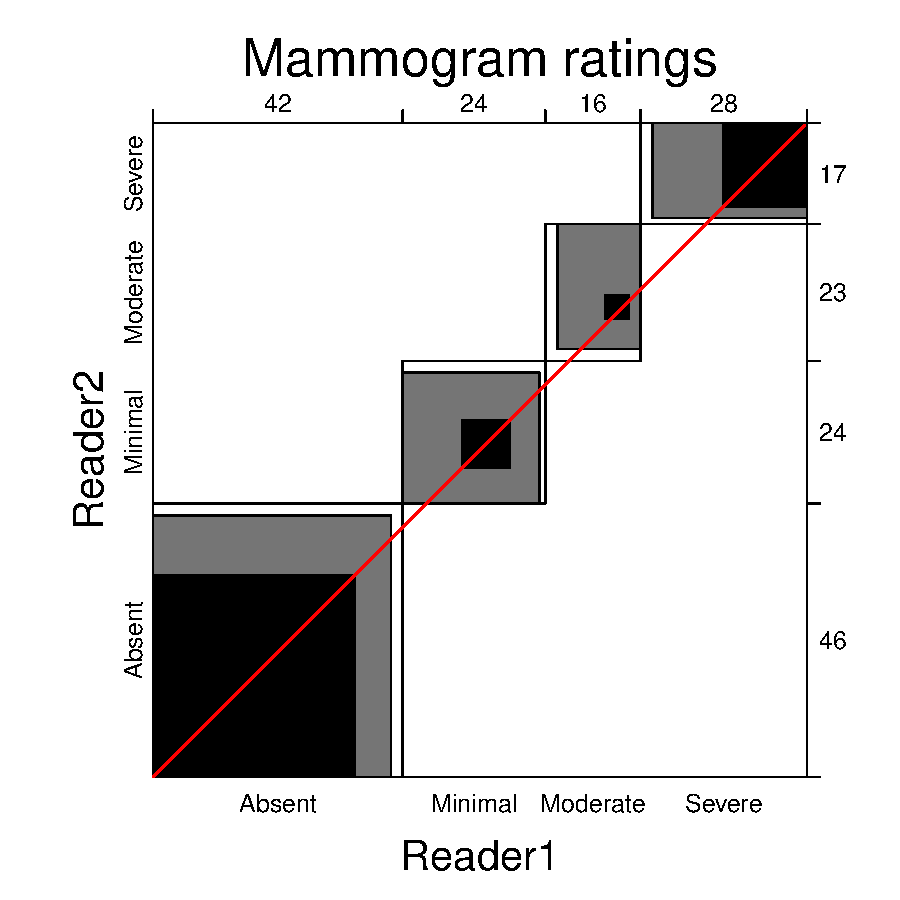
\includegraphics[width=.6\textwidth]{ch04/fig/mammograms1-1} }

\caption[Agreement plot for the Mammograms data]{Agreement plot for the Mammograms data.\label{fig:mammograms1}}
\end{figure}


\end{knitrout}
The agreement plot in \figref{fig:mammograms1} shows substantial agreement
among the two raters, particularly when one-step disagreements are taken into
account.  Careful study of this graph shows that the two raters more often
agree exactly for the extreme categories of ``Absent'' and ``Severe.''
The amounts of unweighted and weighted
agreement are shown numerically in the $B$ and $B^w$
statistics.

\begin{knitrout}
\definecolor{shadecolor}{rgb}{1, 0.961, 0.933}\color{fgcolor}\begin{kframe}
\begin{alltt}
\hlstd{> }\hlkwd{unlist}\hlstd{(B)[}\hlnum{1} \hlopt{:} \hlnum{2}\hlstd{]}
\end{alltt}
\begin{verbatim}
         Bangdiwala Bangdiwala_Weighted 
            0.42721             0.83665 
\end{verbatim}
\end{kframe}
\end{knitrout}


\end{Example}
\subsection{Observer bias in agreement}\label{sec:twoway-observer}

With an ordered scale, it may happen that one observer consistently
tends to classify the objects into higher or lower categories than
the other, perhaps due to using stricter thresholds for the
boundaries between adjacent categories.
This bias produces differences in the marginal totals,
\(n_{i+}\), and \(n_{+i}\) and decreases the maximum possible agreement.
While special tests exist for
\term{marginal homogeneity}, the observer agreement chart shows this
directly by the relation of the dark squares to the diagonal line:
When the marginal totals are the same, the squares fall along the
diagonal.
The measures of agreement, $\kappa$ and $B$, cannot determine
whether lack of agreement is due to such bias, but the agreement chart can
detect this.
%\ix{marginal homogeneity}

\begin{Example}[MS2]{Diagnosis of MS patients}

Agreement charts for both patient samples in the \data{MSPatients} data
are shown in \figref{fig:MS-agree}. The \func{agreementplot} function
only handles two-way tables, so we do these separately by indexing
on the last dimension (\var{Patients}).

\begin{knitrout}
\definecolor{shadecolor}{rgb}{1, 0.961, 0.933}\color{fgcolor}\begin{kframe}
\begin{alltt}
\hlstd{> }\hlkwd{agreementplot}\hlstd{(MSPatients[, ,} \hlstr{"Winnipeg"}\hlstd{],} \hlkwc{main} \hlstd{=} \hlstr{"Winnipeg patients"}\hlstd{)}
\hlstd{> }\hlkwd{agreementplot}\hlstd{(MSPatients[, ,} \hlstr{"New Orleans"}\hlstd{],} \hlkwc{main} \hlstd{=} \hlstr{"New Orleans patients"}\hlstd{)}
\end{alltt}
\end{kframe}\begin{figure}[!htbp]

\centerline{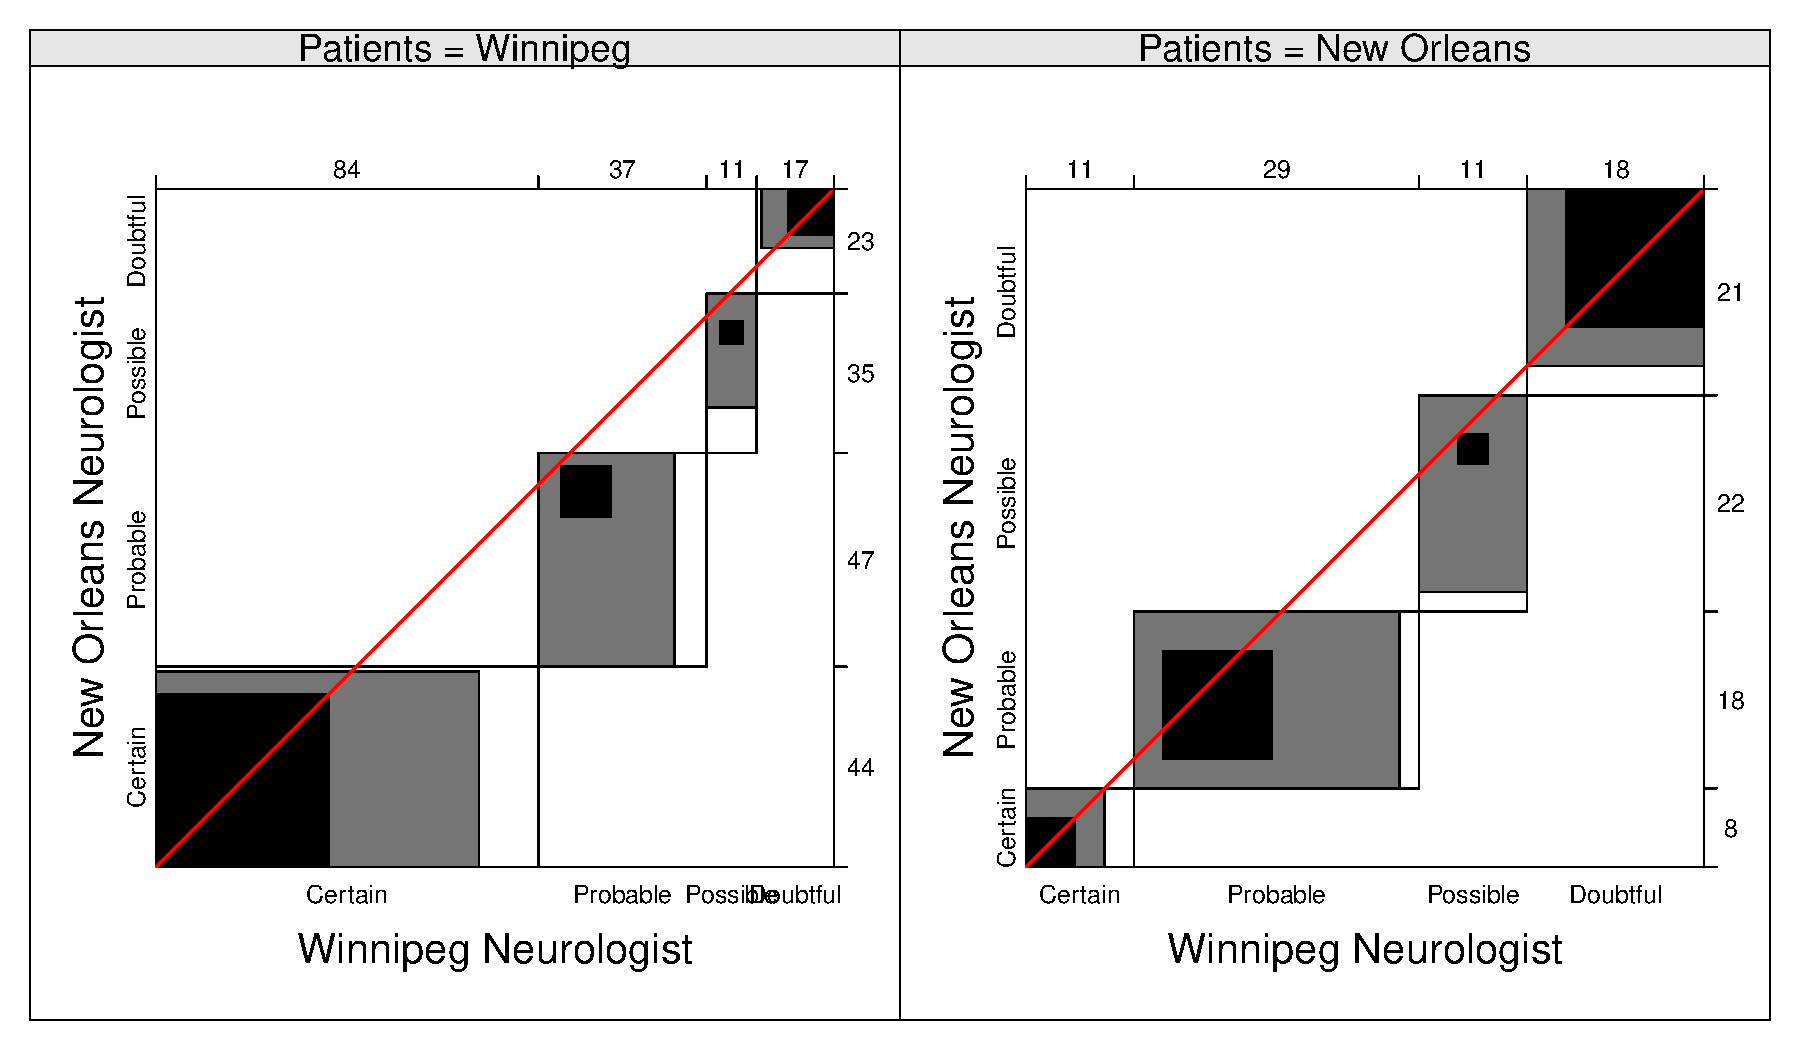
\includegraphics[width=0.49\textwidth]{ch04/fig/MS-agree-1} 
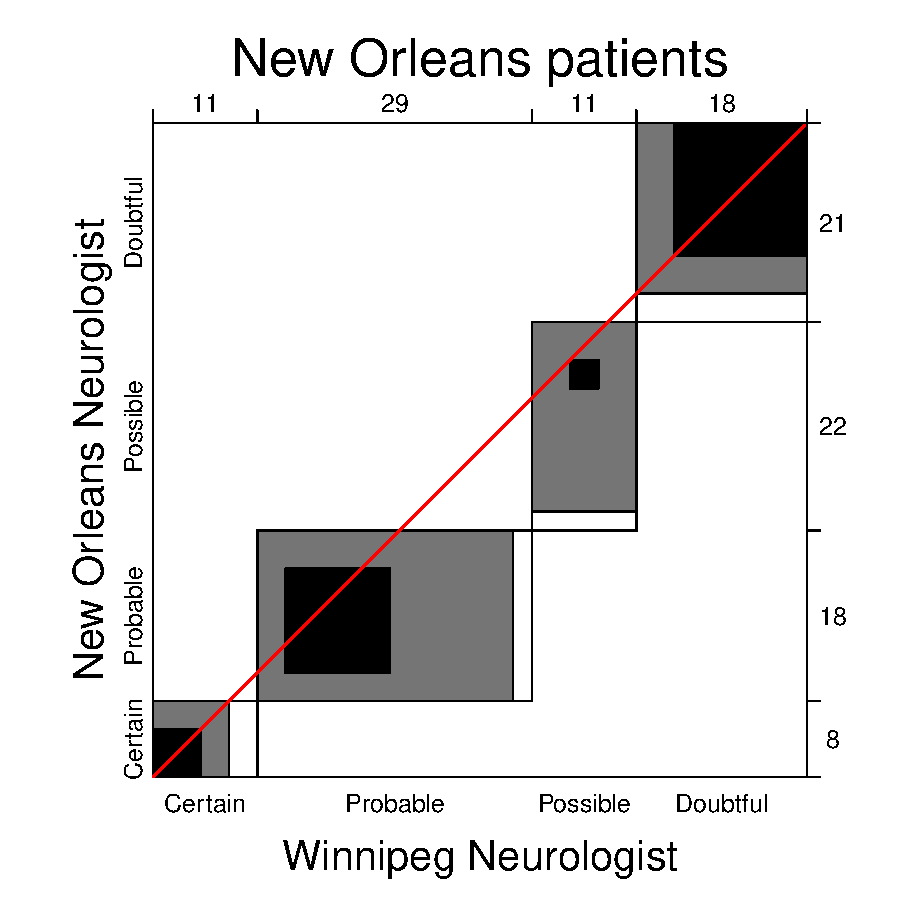
\includegraphics[width=0.49\textwidth]{ch04/fig/MS-agree-2} }

\caption[Weighted agreement charts for both patient samples in the MSPatients data]{Weighted agreement charts for both patient samples in the MSPatients data. Departure of the middle rectangles from the diagonal indicates lack of marginal homogeneity.\label{fig:MS-agree}}
\end{figure}


\end{knitrout}

It can be seen that, for
both groups of patients, the rectangles for the
two intermediate categories lie largely below the diagonal line
(representing equality).  This
indicates that the Winnipeg neurologist tends to classify patients
into more severe diagnostic categories.
The departure from the diagonal is greater for the Winnipeg patients,
for whom the Winnipeg neurologist uses the two most severe diagnostic
categories very often, as can also be seen from the marginal totals
printed in the plot margins.

Nevertheless there is a reasonable amount of agreement if one-step
disagreements are allowed, as can be seen in figref{fig:MS-agree}
and quantified in the $B^w$ statistics below.
The agreement charts also serve to explain why the $B$ measures for
exact agreement are so much lower.
\begin{knitrout}
\definecolor{shadecolor}{rgb}{1, 0.961, 0.933}\color{fgcolor}\begin{kframe}
\begin{alltt}
\hlstd{> }\hlstd{agr1} \hlkwb{<-} \hlkwd{agreementplot}\hlstd{(MSPatients[, ,} \hlstr{"Winnipeg"}\hlstd{])}
\hlstd{> }\hlstd{agr2} \hlkwb{<-} \hlkwd{agreementplot}\hlstd{(MSPatients[, ,} \hlstr{"New Orleans"}\hlstd{])}
\hlstd{> }\hlkwd{rbind}\hlstd{(}\hlkwc{Winnipeg} \hlstd{=} \hlkwd{unlist}\hlstd{(agr1),} \hlkwc{NewOrleans} \hlstd{=} \hlkwd{unlist}\hlstd{(agr2))[,} \hlnum{1} \hlopt{:} \hlnum{2}\hlstd{]}
\end{alltt}
\begin{verbatim}
           Bangdiwala Bangdiwala_Weighted
Winnipeg      0.27210             0.73808
NewOrleans    0.28537             0.82231
\end{verbatim}
\end{kframe}
\end{knitrout}

\ixd{multiple sclerosis diagnosis}


\begin{comment}
\begin{figure}[htb]
\centering
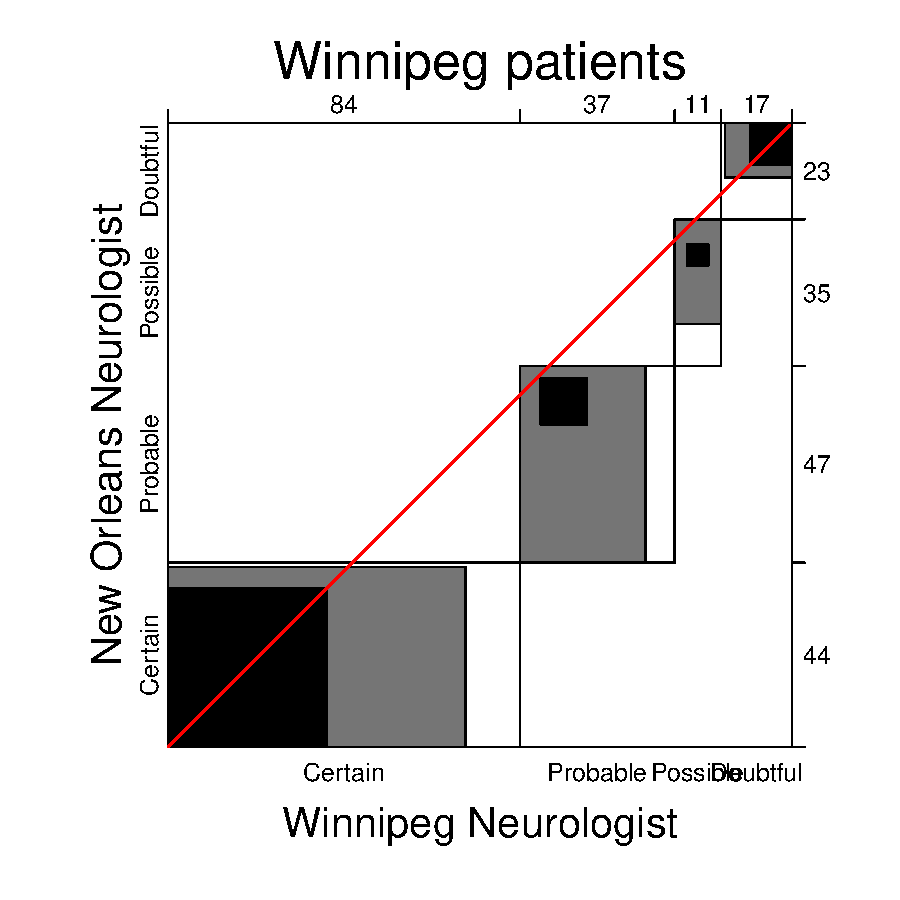
\includegraphics[width=.49\textwidth,clip]{ch04/fig/MSagree1}
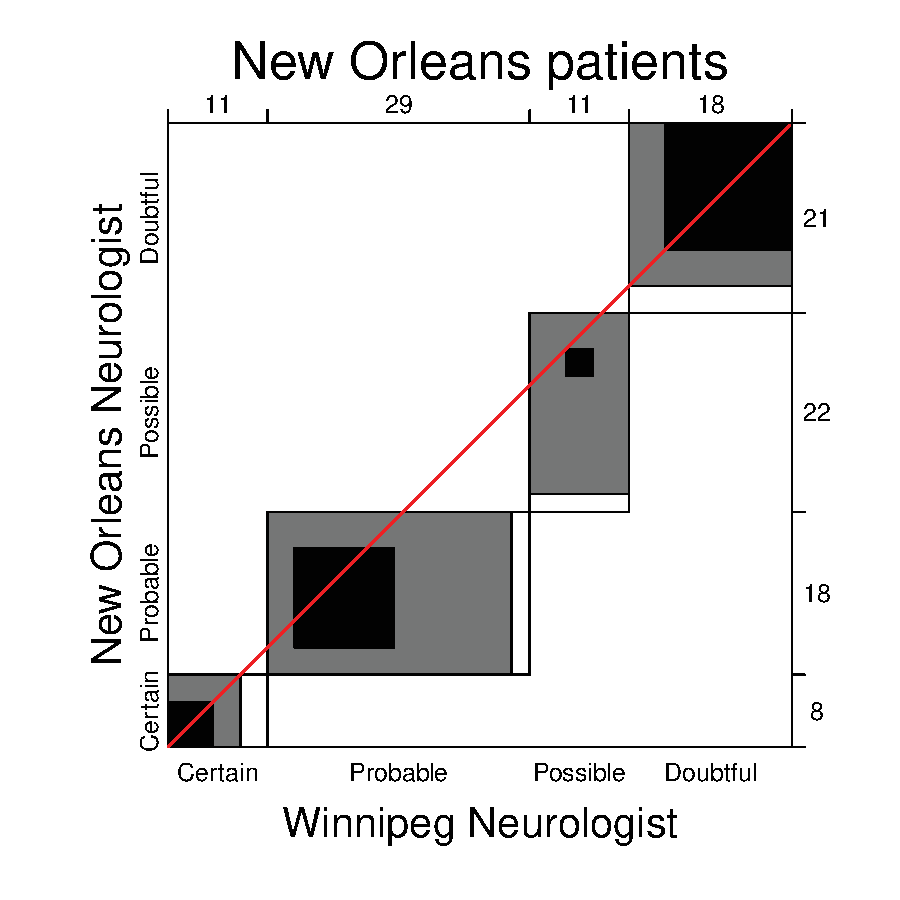
\includegraphics[width=.49\textwidth,clip]{ch04/fig/MSagree2}
\caption{Weighted agreement charts for both patient samples in the MSPatients data. Departure of the middle rectangles from the diagonal indicates lack of marginal homogeneity.}\label{fig:MSagree}
\end{figure}
\end{comment}

\end{Example}

\section{Trilinear plots}\label{sec:twoway-trilinear}

The \term{trilinear plot}
(also called a \emph{ternary diagram} or \emph{trinomial plot})
is a specialized display for a 3-column \ctab or for
three variables whose relative proportions are to be displayed.
Individuals may be assigned to one of three diagnostic categories,
for example, or a chemical process may yield three constituents
in varying proportions, or we may look at the division of votes
among three parties in a parliamentary election.
This display is useful, therefore, for both frequencies
and proportions.

Trilinear plots are featured prominently in \citet{Aitchison:86},
who describes statistical models for this type of
\term{compositional data}.  \citet{Upton:76,Upton:94}
uses them in detailed analyses of spatial and temporal changes in
British general elections.
\citet{Wainer:96} reviews a variety of other uses of trilinear
plots and applies them to aid in understanding the distributions
of students achievement in the
National Assessment of Educational Progress,
making some aesthetic improvements to the traditional form of these
plots along the way.

A trilinear plot displays each observation as a point inside
an equilateral triangle whose coordinate corresponds to the
relative proportions in each column.
The three vertices represent the three extremes when 100\%
occurs in one of the three columns; a point in the exact
center corresponds to equal proportions of $\frac13$ in
all three columns.  In fact, each point represents the (weighted)
barycenter of the triangle, the coordinates representing weights
placed at the corresponding vertices. For instance, \figref{fig:tripdemo2}
shows three points whose compositions of three variables,
A, B, and C are given in the data frame \code{DATA} below.
\begin{knitrout}
\definecolor{shadecolor}{rgb}{1, 0.961, 0.933}\color{fgcolor}\begin{figure}[!htbp]

\centerline{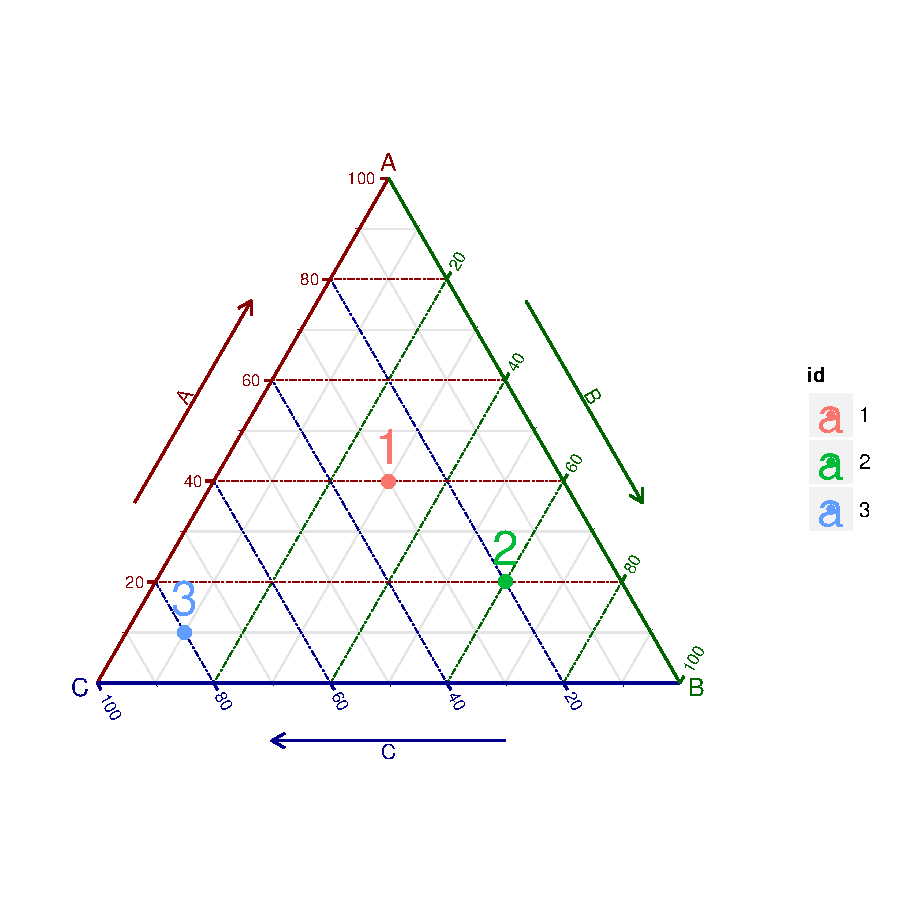
\includegraphics[width=.6\textwidth,trim=20 20 20 20,clip]{ch04/fig/tripdemo2-1} }

\caption[A trilinear plot showing three points, for variables A, B, C]{A trilinear plot showing three points, for variables A, B, C.\label{fig:tripdemo2}}
\end{figure}


\end{knitrout}
\begin{knitrout}
\definecolor{shadecolor}{rgb}{1, 0.961, 0.933}\color{fgcolor}\begin{kframe}
\begin{alltt}
\hlstd{> }\hlkwd{library}\hlstd{(ggtern)}
\hlstd{> }\hlstd{DATA} \hlkwb{<-} \hlkwd{data.frame}\hlstd{(}
\hlstd{+ }  \hlkwc{A} \hlstd{=} \hlkwd{c}\hlstd{(}\hlnum{40}\hlstd{,} \hlnum{20}\hlstd{,} \hlnum{10}\hlstd{),}
\hlstd{+ }  \hlkwc{B} \hlstd{=} \hlkwd{c}\hlstd{(}\hlnum{30}\hlstd{,} \hlnum{60}\hlstd{,} \hlnum{10}\hlstd{),}
\hlstd{+ }  \hlkwc{C} \hlstd{=} \hlkwd{c}\hlstd{(}\hlnum{30}\hlstd{,} \hlnum{20}\hlstd{,} \hlnum{80}\hlstd{),}
\hlstd{+ }  \hlkwc{id} \hlstd{=} \hlkwd{c}\hlstd{(}\hlstr{"1"}\hlstd{,} \hlstr{"2"}\hlstd{,} \hlstr{"3"}\hlstd{))}
\hlstd{> }
\hlstd{> }\hlstd{aesthetic_mapping} \hlkwb{<-} \hlkwd{aes}\hlstd{(}\hlkwc{x} \hlstd{= C,} \hlkwc{y} \hlstd{= A,} \hlkwc{z} \hlstd{= B,} \hlkwc{label} \hlstd{= id,} \hlkwc{colour} \hlstd{= id)}
\hlstd{> }\hlkwd{ggtern}\hlstd{(}\hlkwc{data} \hlstd{= DATA,} \hlkwc{mapping} \hlstd{= aesthetic_mapping)} \hlopt{+}
\hlstd{+ }    \hlkwd{geom_point}\hlstd{(}\hlkwd{aes}\hlstd{(}\hlkwc{size} \hlstd{=} \hlnum{2}\hlstd{))} \hlopt{+}
\hlstd{+ }    \hlkwd{theme_rgbw}\hlstd{()}
\end{alltt}
\end{kframe}
\end{knitrout}
\noindent (The plot shown requires some more cosmetic parameters not
shown for simplicity).

Note that each apex corresponds to 100\% of the labeled
variable, and the percentage of this variable decrease
linearly along a line to the midpoint of the opposite
baseline.
The grid lines in the figure show the percentage value along
each axis.

The construction of trilinear plots is described in detail
in \url{http://en.wikipedia.org/wiki/Ternary_plot}.
Briefly, let $P(a, b, c)$ represent the three components  normalized so
that $a + b + c = 1.0$.
If the apex corresponding to Point A in \figref{fig:tripdemo2}
is given $(x, y)$ coordinates of $(x_A, y_A) = (0, 0)$,
and those at apex B are $(x_B, y_B) = (100, 0)$,
then the coordinates of apex C are $(x_C, y_C) = (50, 50\sqrt{3})$.
The cartesian coordinates $(x_P, y_P)$  of point $P$ are then calculated as
\begin{eqnarray*}
y_P & = & c \: y_C \\
x_P & = & y_P \left( \frac{y_C - y_B}{x_C - x_B} \right)
+ \frac{\sqrt{3}}{2} y_C (1 - a) \\
\end{eqnarray*}

In \R, trilinear plots are implemented in the
\func{triplot} function in the \Rpackage{TeachingDemos},
and also in the \Rpackage{ggtern}, an extension of
the \pkg{ggplot2} framework.  The latter is much more
flexible, because it inherits all of the capabilities
of \pkg{ggplot2} for plot annotations, faceting, and layers.
In essence,
the function \func{ggtern} is just a wrapper for
\code{ggplot(...)} which adds a change in the coordinate
system from cartesian (x, y) coordinates to the
ternary coordinate system with \verb|coord_tern()|.
% For example, the following code%
% \footnote{
% This example was taken from the ggtern web site,
% \url{http://ggtern.com/2013/12/12/patched-density-functions-2/}.
% }
% creates a data frame
% \code{DATA} containing 100 uniformly distributed
% random points.  It uses \verb|stat_density2d()|
% to draw contours of the densities of the points in the
% trilinear space.
% <<ggterm-demo, h=6, w=6, out.width='.6\\textwidth', cap='A trilinear plot with density contours', out.extra='trim=20 20 20 20,clip'>>=
% set.seed(1)
% DATA <- data.frame(x = runif(100),
%                    y = runif(100),
%                    z = runif(100))
% plot <- ggtern(data = DATA,
%                aes(x, y, z))
% plot + stat_density2d(method = "lm", fullrange = T,
%                       n = 200, geom = "polygon",
%                       aes(fill = ..level..,
%                           alpha = ..level..)) +
%     geom_point() +
%     theme_tern_rgbw() +
%     labs(title = "Uniform data with density contours")    +
%     scale_fill_gradient(low = "blue",high = "red")  +
%     guides(color = "none", fill = "none", alpha = "none")
% @

\begin{Example}[lifeboat1]{Lifeboats on the \emph{Titanic}}
We examine the question of who survived and why in the sinking of the \emph{RMS Titanic} in \secref{sec:mosaic-threeway} (\exref{ex:titanic}),
where we analyze a four-way table, \data{Titanic},
of the $2,201$ people on board ($1,316$ passengers and 885 crew),
classified by \var{Class}, \var{Sex}, \var{Age}, and \var{Survival}.
\TODO{This Titanic example does not yet exist in chapter 5!}
A related \Dset, \data{Lifeboats} in \pkg{vcd}, tabulates
the survivors according to the life boats on which they were loaded.
This data sheds some additional light on the issue of survival and
provides a nice illustration of trilinear plots.

A bit of background: after the disaster, the British Board of Trade launched several
inquiries, the most comprehensive of which resulted in the
\emph{Report on the Loss of the ``Titanic'' (S.S.)}
by Lord Mersey
\citep{Mersey:1912}.
\footnote{
%Section 4 of this document contains a detailed account of the saving
%and rescue of the passengers and crew who survived.
The \emph{Titanic} was outfitted with 20 boats, half on each of the
port and starboard sides,
 of which 14 were large
lifeboats with a capacity of 65, two were emergency boats designed for
40 persons, and the remaining four were collapsible boats capable of holding
47, a total capacity of $1,178$ (considered adequate at that time).
Two of the collapsible boats, lashed to the roof of the officers
quarters, were ineffectively launched and utilized as rafts after the ship sunk.
The report lists the time of launch and composition of the remaining 18 boats according to male passengers, women and children, and ``men of crew'',
as reported by witnesses.
}
The  data frame \data{Lifeboats}  in \pkg{vcd}
contains the data listed on p. 38 of that report.%
\footnote{The ``data'' lists a total of 854 in 18 boats, although only
712 were in fact saved.  Mersey notes ``it is obvious that these figures
are quite unreliable''.
%Allowing for 60 people rescued from the water,
%only 652 could have left in the boats \citep[p. 39]{Mersey:1912}.
%We present an alternative \Dset, \pname{LIFEBOA2}, in \datref{dat:lifeboat},
%based on more conservative and historically accurate information.
}

Of interest here is the composition of the boats by the three categories:
men, women and children, and crew,
and according to the launching of the boats from the port or starboard
side. This can be shown in a trilinear display
using the following statements.
The plot, shown in
\figref{fig:lifeboats1}, has most of the points near the bottom left,
corresponding to a high percentage of women and children.
We create a variable, \var{id}, used to label those boats
with more than 10\% male passengers.  In the \code{ggplot2}
framework, plot aesthetics, such as color and shape can be
mapped to variables in the data set, and here we map these
both to \code{side} of the boat.
\begin{knitrout}
\definecolor{shadecolor}{rgb}{1, 0.961, 0.933}\color{fgcolor}\begin{kframe}
\begin{alltt}
\hlstd{> }\hlkwd{data}\hlstd{(}\hlstr{"Lifeboats"}\hlstd{,} \hlkwc{package} \hlstd{=} \hlstr{"vcd"}\hlstd{)}
\hlstd{> }\hlcom{# label boats with more than 10% men}
\hlstd{> }\hlstd{Lifeboats}\hlopt{$}\hlstd{id} \hlkwb{<-} \hlkwd{ifelse}\hlstd{(Lifeboats}\hlopt{$}\hlstd{men} \hlopt{/} \hlstd{Lifeboats}\hlopt{$}\hlstd{total} \hlopt{>} \hlnum{.1}\hlstd{,}
\hlstd{+ }                       \hlkwd{as.character}\hlstd{(Lifeboats}\hlopt{$}\hlstd{boat),} \hlstr{""}\hlstd{)}
\hlstd{> }                       
\hlstd{> }\hlstd{AES} \hlkwb{<-} \hlkwd{aes}\hlstd{(}\hlkwc{x} \hlstd{= women,} \hlkwc{y} \hlstd{= men,} \hlkwc{z} \hlstd{= crew,} \hlkwc{colour} \hlstd{= side,} \hlkwc{shape} \hlstd{= side,} \hlkwc{label} \hlstd{= id)}
\hlstd{> }\hlkwd{ggtern}\hlstd{(}\hlkwc{data} \hlstd{= Lifeboats,} \hlkwc{mapping} \hlstd{= AES)} \hlopt{+}
\hlstd{+ }     \hlkwd{geom_text}\hlstd{()} \hlopt{+}
\hlstd{+ }     \hlkwd{theme_rgbw}\hlstd{()} \hlopt{+}
\hlstd{+ }     \hlkwd{geom_smooth}\hlstd{(}\hlkwc{method} \hlstd{=} \hlstr{"lm"}\hlstd{,} \hlkwc{alpha} \hlstd{=} \hlnum{0.2}\hlstd{)}
\end{alltt}
\end{kframe}
\end{knitrout}
\begin{knitrout}
\definecolor{shadecolor}{rgb}{1, 0.961, 0.933}\color{fgcolor}\begin{figure}[!htbp]

\centerline{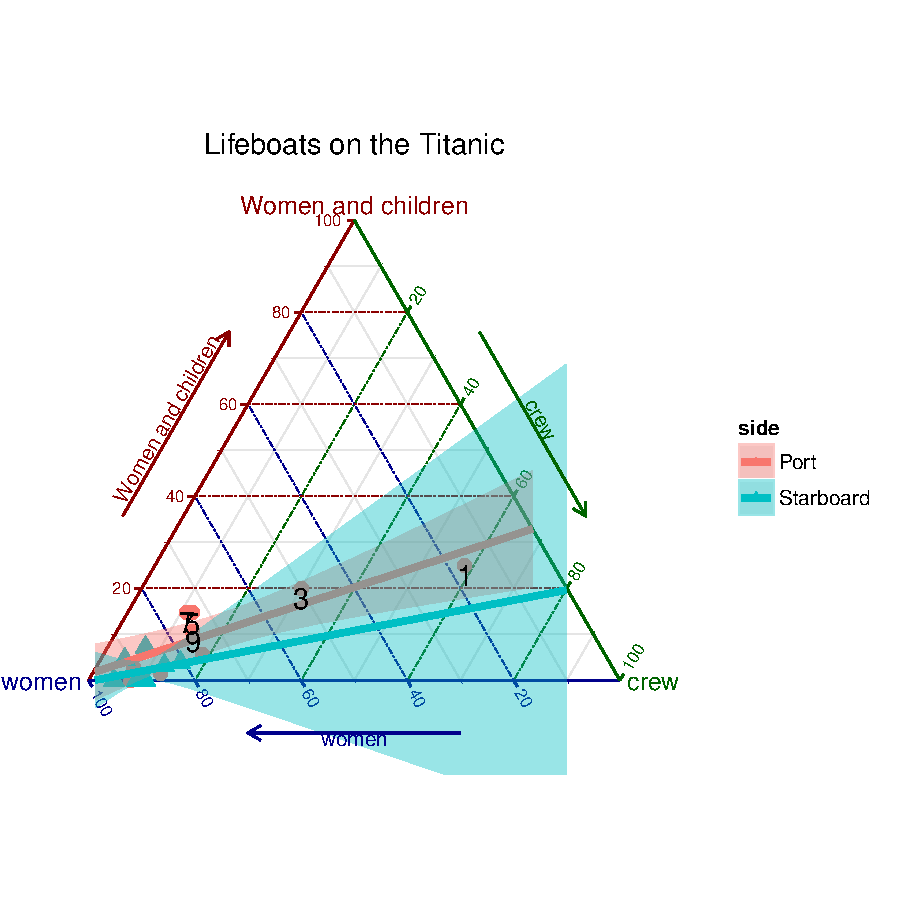
\includegraphics[width=.7\textwidth,clip,trim=0 80 0 80]{ch04/fig/lifeboats1-1} }

\caption[Lifeboats on the Titanic]{Lifeboats on the \emph{Titanic}, showing the composition of each boat.  Boats with more than 10\% male passengers are labeled.\label{fig:lifeboats1}}
\end{figure}


\end{knitrout}
The resulting plot in \figref{fig:lifeboats1} (for which some more cosmetic
parameters than shown in the code above have been used) makes it immediately apparent
that many of the boats launched from the port side differ substantially
from the starboard boats, whose passengers were almost entirely women
and children.  Boat 1 had only 20\% (2 out of 10) women and children, while the percentage for boat 3 was only 50\% (25 out of 50). We highlight the difference in
composition of the boats launched from the two sides by adding a linear regression
smooth for the relation \verb|men ~ women|.

The trilinear plot scales the numbers for each observation to sum
to 1.0, so differences in the total number of people on each boat
cannot be seen in \figref{fig:lifeboats1}.
The \code{total} number reported loaded is plotted against
\code{launch} time in \figref{fig:lifeboats2},
with a separate regression line and loess smooth
fit to the data for the port and starboard
sides (code again simplified for clarity):
\begin{knitrout}
\definecolor{shadecolor}{rgb}{1, 0.961, 0.933}\color{fgcolor}\begin{kframe}
\begin{alltt}
\hlstd{> }\hlstd{AES} \hlkwb{<-} \hlkwd{aes}\hlstd{(}\hlkwc{x} \hlstd{= launch,} \hlkwc{y} \hlstd{= total,} \hlkwc{colour} \hlstd{= side,} \hlkwc{label} \hlstd{= boat)}
\hlstd{> }\hlkwd{ggplot}\hlstd{(}\hlkwc{data} \hlstd{= Lifeboats,} \hlkwc{mapping} \hlstd{= AES)} \hlopt{+}
\hlstd{+ }     \hlkwd{geom_text}\hlstd{()} \hlopt{+}
\hlstd{+ }     \hlkwd{geom_smooth}\hlstd{(}\hlkwc{method} \hlstd{=} \hlstr{"lm"}\hlstd{,} \hlkwd{aes}\hlstd{(}\hlkwc{fill} \hlstd{= side),} \hlkwc{size} \hlstd{=} \hlnum{1.5}\hlstd{)} \hlopt{+}
\hlstd{+ }     \hlkwd{geom_smooth}\hlstd{(}\hlkwc{method} \hlstd{=} \hlstr{"loess"}\hlstd{,} \hlkwd{aes}\hlstd{(}\hlkwc{fill} \hlstd{= side),} \hlkwc{se} \hlstd{=} \hlnum{FALSE}\hlstd{,} \hlkwc{size} \hlstd{=} \hlnum{1.2}\hlstd{)}
\end{alltt}
\end{kframe}
\end{knitrout}
\begin{knitrout}
\definecolor{shadecolor}{rgb}{1, 0.961, 0.933}\color{fgcolor}\begin{figure}[!htbp]

\centerline{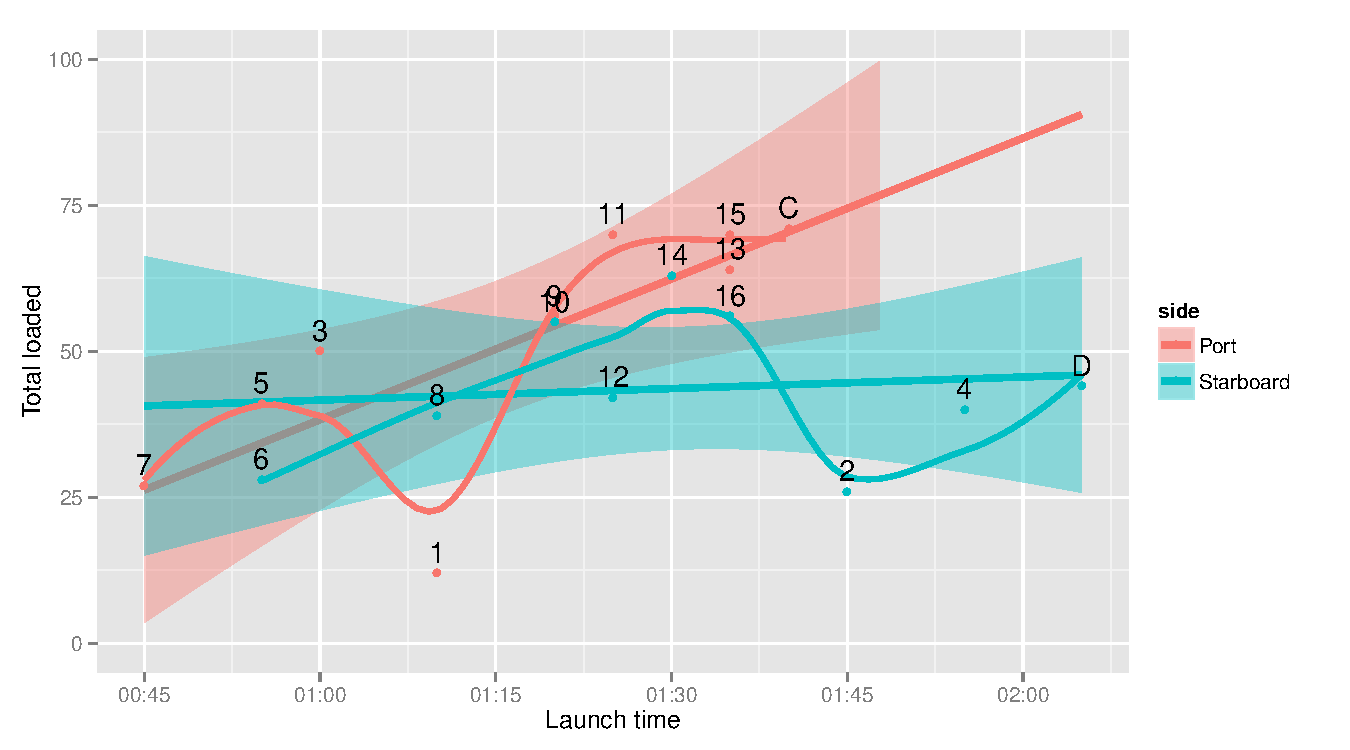
\includegraphics[width=.8\textwidth]{ch04/fig/lifeboats2-1} }

\caption[Number of people loaded on lifeboats on the Titanic vs]{Number of people loaded on lifeboats on the Titanic vs. time of launch, by side of boat. The plot annotations show the linear regression and loess smooth.\label{fig:lifeboats2}}
\end{figure}


\end{knitrout}
From the linear regression lines in \figref{fig:lifeboats2},
it seems that the rescue effort began in panic on the port side,
with relatively small numbers loaded, and (from \figref{fig:lifeboats1}),
small proportions of women and children.
But the loading regime on that side improved steadily over time.
The procedures began more efficiently on the starboard side
but the numbers loaded increased only slightly.
The smoothed loess curves indicate that over time, for each side,
there was still a large variability from boat to boat.

\end{Example}


\section{Chapter summary}\label{sec:twoway-summary}

\begin{itemize}
  \item A \ctab gives the frequencies of observations
  cross-classified by two or more categorical variables.
%  Different types of variables may be distinguished, such as
%  response, explanatory and stratifying variables.
  With such data we are typically interested in testing whether
  associations exist, quantifying the strength of association,
  and understanding the nature of the association among these
  variables.

  \item For $2 \times 2$ tables, association is
   easily summarized in terms of the odds ratio or its logarithm.
   This measure can be extended to stratified $2 \times 2 \times k$
   tables, where we can also assess whether the odds ratios are
   equal across strata or how they vary.

  \item For $r \times c$ tables, measures and
  tests of general association between two categorical variables are
  most typically carried out using the Pearson's chi-squared or
  \LR tests provided by \func{assocstats}.
  Stratified tests controlling for one or more background variables, and
  tests for ordinal categories are provided by the
  Cochran-Mantel-Haenszel tests given by \func{CMHtest}.

  \item For $2 \times 2$ tables, the fourfold display provides a
  visualization of the association between variables in terms of
  the odds ratio.  Confidence rings provide a visual test of
  whether the odds ratio differs significantly from 1. Stratified
  plots for $2 \times 2 \times k$ tables are also provided by \func{fourfold}.

  \item Sieve diagrams and association plots provide other useful displays of the pattern of association in $r \times c$ tables.  These also extend to higher-way tables
  as part of the strucplot framework.

  \item When the row and column variables represent different
  observers rating the same subjects, interest is focused on
  agreement rather than mere association.  Cohen's $\kappa$ is one
  measure of strength of agreement.  The observer agreement chart
  provides a visual display of how the observers agree and
  disagree.

  \item Another specialized display, the trilinear plot is useful
  for three-column frequency tables or compositional data.
\end{itemize}


\section{Further reading}\label{sec:twoway-reading}

\section{Lab exercises}\label{sec:twoway-lab}

%\section{Lab exercises}\label{sec:twoway-lab}

\begin{Exercises}

  \exercise The data set \code{fat}, created below, gives a $2 \times 2$ table recording the level of
  cholesterol in diet and the presence of symptoms of heart disease for a sample of
  23 people.

\begin{knitrout}
\definecolor{shadecolor}{rgb}{1, 0.961, 0.933}\color{fgcolor}\begin{kframe}
\begin{alltt}
\hlstd{> }\hlstd{fat} \hlkwb{<-} \hlkwd{matrix}\hlstd{(}\hlkwd{c}\hlstd{(}\hlnum{6}\hlstd{,} \hlnum{4}\hlstd{,} \hlnum{2}\hlstd{,} \hlnum{11}\hlstd{),} \hlnum{2}\hlstd{,} \hlnum{2}\hlstd{)}
\hlstd{> }\hlkwd{dimnames}\hlstd{(fat)} \hlkwb{<-} \hlkwd{list}\hlstd{(}\hlkwc{diet} \hlstd{=} \hlkwd{c}\hlstd{(}\hlstr{"LoChol"}\hlstd{,} \hlstr{"HiChol"}\hlstd{),}
\hlstd{+ }                      \hlkwc{disease} \hlstd{=} \hlkwd{c}\hlstd{(}\hlstr{"No"}\hlstd{,} \hlstr{"Yes"}\hlstd{))}
\end{alltt}
\end{kframe}
\end{knitrout}

  \begin{enumerate*}
    \item Use \code{chisq.test(fat)} to test for association between diet and disease.
    Is there any indication that this test may not be appropriate here?
    \item Use a fourfold display to test this association visually.  Experiment with
    the different options for standardizing the margins, using the \code{margin}
    argument to \func{fourfold}. What evidence is shown in different displays regarding
    whether the odds ratio differs significantly from 1?
    \item \code{oddsratio(fat, log = FALSE)} will give you a numerical answer.  How does
    this compare to your visual impression from fourfold displays?
    \item With such a small sample, Fisher's exact test may be more reliable for statistical
    inference.  Use \code{fisher.test(fat)}, and compare these results to what you have
    observed before.
    \item Write a one-paragraph summary of your findings and conclusions for this data set.
  \end{enumerate*}

  \exercise The data set \data{Abortion} in \pkg{vcdExtra} gives a $2 \times 2 \times 2$
  table of opinions regarding abortion in relation to sex and status of the
  respondent. This table has the following structure:
\begin{knitrout}
\definecolor{shadecolor}{rgb}{1, 0.961, 0.933}\color{fgcolor}\begin{kframe}
\begin{alltt}
\hlstd{> }\hlkwd{data}\hlstd{(}\hlstr{"Abortion"}\hlstd{,} \hlkwc{package}\hlstd{=}\hlstr{"vcdExtra"}\hlstd{)}
\hlstd{> }\hlkwd{str}\hlstd{(Abortion)}
\end{alltt}
\begin{verbatim}
 table [1:2, 1:2, 1:2] 171 152 138 167 79 148 112 133
 - attr(*, "dimnames")=List of 3
  ..$ Sex             : chr [1:2] "Female" "Male"
  ..$ Status          : chr [1:2] "Lo" "Hi"
  ..$ Support_Abortion: chr [1:2] "Yes" "No"
\end{verbatim}
\end{kframe}
\end{knitrout}
  \begin{enumerate*}
    \item Taking support for abortion as the outcome variable, produce fourfold displays
    showing the association with sex, stratified by status.
    \item Do the same for the association of support for abortion with status, stratified
    by sex.
    \item For each of the problems above, use \func{oddsratio} to calculate the numerical
    values of the odds ratio, as stratified in the question.
    \item Write a brief summary of how support for abortion depends on sex and status.
  \end{enumerate*}

  \exercise The \data{JobSat} table on income and job satisfaction
  created in \exref{ex:jobsat1} is contained in the
  \Rpackage{vcdExtra}.
  \begin{enumerate*}
    \item Carry out a standard $\chi^2$ test for association between income and job satisfaction.
    Is there any indication that this test might not be appropriate?
      Repeat this test using \code{simulate.p.value = TRUE} to obtain a Monte Carlo
      test that does not depend on large sample size.  Does this change your
      conclusion?
    \item Both variables are ordinal, so CMH tests may be more powerful here.
    Carry out that analysis.  What do you conclude?
  \end{enumerate*}

  \exercise The \data{Hospital} data in \pkg{vcd} gives a $3 \times 3$ table
  relating the length of stay (in years) of 132 long-term schizophrenic patients in two London mental hospitals with the frequency of visits
  by family and friends.
    \begin{enumerate*}
      \item Carry out a  $\chi^2$ test for association between the two
      variables.
      \item Use \func{assocstats} to compute association statistics.
      How would you describe the strength of association here?
      \item Produce an association plot for these data, with
      visit frequency as the vertical variable.  Describe the
      pattern of the relation you see here.
      \item Both variables can be considered ordinal, so
      \func{CMHtest} may be useful here.  Carry out that
      analysis.  Do any of the tests lead to different conclusions?
    \end{enumerate*}

  \exercise Continuing with the \data{Hospital} data:
    \begin{enumerate*}
      \item Try one or more of the following other functions for visualizing two-way contingency tables with this data: 
      \func{plot}, \func{tile}, \func{mosaic}, and \func{spineplot}.  
      [For all except spineplot(), it is useful to include the argument shade=TRUE].
      \item Comment on the differences among these displays for understanding the relation between visits and length of stay.
    \end{enumerate*}
  
  \exercise The two-way table \data{Mammograms} in \pkg{vcdExtra} gives ratings
  on the severity of diagnosis of 110 mammograms by two raters.
    \begin{enumerate*}
      \item Assess the strength of agreement between the raters using Cohen's
      $\kappa$, both unweighted and weighted.
      \item Use \func{agreementplot} for a graphical display of agreement here.
      \item Compare the Kappa measures with the results from \func{assocstats}. 
      What is a reasonable interpretation of each of these measures?
    \end{enumerate*}

  \exercise \citet{AgrestiWinner:1997} gave the data in \tabref{tab:siskel-ebert} on the
  ratings of 160 movies by the reviewers Gene Siskel and Roger Ebert for the period
  from April 1995 through September 1996. The rating categories were Con (``thumbs down''),
  Mixed, and Pro (``thumbs up'').
  \begin{table}[!htb]
\centering
\caption{Movie ratings by Siskel \& Ebert, April 1995--September 1996. \emph{Source}: \citet{AgrestiWinner:1997}}\label{tab:siskel-ebert}
\begin{tabular}{rr|lll|l}
        &       &  \multicolumn{3}{|c|}{Ebert} \\
        &       & Con & Mixed & Pro & Total \\ \hline
        & Con   &  24 &   8   &  13 &  45   \\
 Siskel & Mixed &   8 &  13   &  11 &  32   \\
        & Pro   &  10 &   9   &  64 &  83   \\ \hline
        & Total &  42 &  30   &  88 & 160   \\
\end{tabular}
\end{table}
  \begin{enumerate*}
     \item Assess the strength of agreement between the raters using Cohen's
       $\kappa$, both unweighted and weighted.
     \item Use \func{agreementplot} for a graphical display of agreement here.
     \item Assess the hypothesis that the ratings are \emph{symmetric} around the
       main diagonal, using an appropriate $\chi^2$ test.
       \emph{Hint}:  Symmetry for a square table $\mat{T}$ means that $t_{ij} = t_{ji}$
       for $i \ne j$.  The expected frequencies under the hypothesis of symmetry
       are the average of the off-diagonal cells,
       $\mat{E} = (\mat{T} + \mat{T}\trans) / 2$.
     \item Compare the results with the output of \func{mcnemar.test}.
     \end{enumerate*}

  \exercise For the \data{VisualAcuity} data set:
    \begin{enumerate*}
      \item Use the code shown in the text to create the table form, \code{VA.tab}.
      \item Perform the CMH tests for this table.
      \item Use the \func{woolf\_test} described in \secref{sec:twoway-homog} to
      test whether the association between left and right eye acuity can be
      considered the same for men and women.
    \end{enumerate*}

  \exercise The graph in \figref{fig:lifeboats2} may be misleading, in that it doesn't
  take into account of the differing capacities of the 18 life boats on the
  \emph{Titanic}, given in the variable \var{cap} in the \data{Lifeboats} data.
    \begin{enumerate*}
      \item Calculate a new variable, \code{pctloaded} as the percentage
      loaded relative to the boat capacity.
      \item Produce a plot similar to \figref{fig:lifeboats2}, showing the
      changes over time in this measure.
    \end{enumerate*}

\end{Exercises}














%%%%%%%%%%%%%%%%%%%%%%%%%%%%%%%%%%%%%%%%%%%%%%%%%%%%%%%%%%%%%%%%%%%%%%%%%


% To resolve citations in the chapter, ...
{\itemsep -1pt
\bibliography{graphics,statistics,timeref,Rpackages}
%%% Use aux2bib to process the .aux file, creating references.bib
%%% Then change to line below
%\bibliography{references}
}

% \newpage
% This document was produced using:
% 
% <<session-info>>=
% print(sessionInfo(), locale = FALSE)
% @

	
%%%%% THE END %%%%%
\end{document}

